% 高一24_复旦附中_周末作业3.tex
%   —— 高一上数学「2026-2027 年复旦附中高一上周末作业 3」（试卷版/答案版）
% 试卷版：xelatex 高一24_复旦附中_周末作业3.tex
% 答案版：xelatex "\def\isanswer{1}% 高一24_复旦附中_周末作业3.tex
%   —— 高一上数学「2026-2027 年复旦附中高一上周末作业 3」（试卷版/答案版）
% 试卷版：xelatex 高一24_复旦附中_周末作业3.tex
% 答案版：xelatex "\def\isanswer{1}% 高一24_复旦附中_周末作业3.tex
%   —— 高一上数学「2026-2027 年复旦附中高一上周末作业 3」（试卷版/答案版）
% 试卷版：xelatex 高一24_复旦附中_周末作业3.tex
% 答案版：xelatex "\def\isanswer{1}% 高一24_复旦附中_周末作业3.tex
%   —— 高一上数学「2026-2027 年复旦附中高一上周末作业 3」（试卷版/答案版）
% 试卷版：xelatex 高一24_复旦附中_周末作业3.tex
% 答案版：xelatex "\def\isanswer{1}\input{高一24_复旦附中_周末作业3.tex}"
% 紧凑版：xelatex "\def\iscompact{1}\input{高一24_复旦附中_周末作业3.tex}"
%
% 原始材料是微信公众号图文（公众号「魔都数学加油站」连载「27学年高一 24」，2026-09-19 发布，
% 原文标题「27学年高一24——2026-2027年上海市复旦附中高一上周末作业3集合与逻辑、等式的性质」），
% 正文为 7 张 PNG 页（1080×1527，各页同尺寸）。原文本身就是一份**讲评版**——题目下方直接印出
% 【答案】或【解析】。试题文字、答案与解析均照原卷录入，未改内容。
% 卷面上的粉色斜水印「魔都数学加油站」属水印，未录入。
%
% 卷首标题：原卷印作「2026-2027 年复旦附中高一上周末作业 3」（公众号标题里有「上海市」三字，
% 卷面标题行没有，本稿照卷面），年份区间按全稿惯例排 en dash，前缀照原卷保留「年」。
%
% 与原卷的排版差异（均已在 README「说明」中交代）：
%   ① 原文自**第 3 题**起（第 1、2 题未在该文中发布），故本稿题号亦自 3 起；
%   ② 原卷本就印有「一、填空题」「二、选择题」「三、解答题」三节标题，本稿照原卷分节，
%      只把标题改排成全稿统一的「大节标题」样式；
%   ③ 原卷第 11 题的答案「A」直接印在题干末尾的括号内，第 12、13 题的括号空着、答案写在
%      解析末句「故选 C／D」里，本稿统一改为试卷版隐去、答案版以 \ans{} 给出（第 12、13 题
%      另附【解析】），使两版彻底分离；
%   ④ 原卷的集合／数集符号正体与粗体混用（第 8 题题干的 $\mathbf{R}$、第 9 题题干的
%      $\mathbf{N}$、第 12 题题干的 $\mathbf{Z}$ 为粗体，第 14 题解析的 $N$、$R$ 为斜体），
%      本稿按全稿惯例统一写作 $\R$、$\N$、$\Z$；
%   ⑤ 原卷填空的横线约两个字宽，本稿按全稿惯例统一排 \blankline[4.4em]；
%   ⑥ 第 11 题的 Venn 图原卷印在上一页末尾（第 10 题解析右侧、「二、选择题」标题旁），
%      本稿移至第 11 题题干之后；图取原卷截图、4× LANCZOS 放大
%      （figures/venn_ABcap_plus_C.png，阴影为 $A\cap B$ 的交与整个 $C$，即 $(A\cap B)\cup C$）；
%   ⑦ 原卷自印副标题「集合与逻辑、等式的性质」，本稿照录（与 高一14 同例，未改用惯例副标题）；
%   ⑧ 第 14 题题干原卷把「$=0$」印在右花括号**之外**（作
%      $A=\{x\mid x^2-mx+4m-16\}=0$），而它**自己的【解析】却印在括号之内**
%      （作 $A=\{x\mid x^2-mx+4m-16=0\}$）——原卷前后不一致；按原卷解析与题目本意，
%      本稿题干的 $=0$ 排在括号**之内**（与 高一b 第 13 题「原卷漏排 $A=$，本稿补上」同例）。
%
% 原卷存疑一处（已放大到能看清字形后核对，无法确证原意，本稿照抄原卷、未改）：
%   ① 第 15(2)【解析】的连等式印作
%      $\left(\frac ba\right)^2-\frac ca=\frac{b^2-ac}{a^2}=\left(\frac ba\right)^2-\frac ba+1=1$，
%      解得 $\frac ba=0$ 或 $-1$（舍去）——但由 $c=-a-b$ 应得 $\frac{b^2-ac}{a^2}
%      =\left(\frac ba\right)^2+\frac ba+1$（原卷把「$+\frac ba$」印成了「$-\frac ba$」）：
%      按原卷那行解出的是 $0$ 或 $1$，与其自己的结论「$0$ 或 $-1$」对不上；而按
%      $+\frac ba$ 解恰得 $0$ 或 $-1$（$-1$ 因 $c<0$ 舍去），与后文吻合。原卷显系笔误，
%      本稿照抄原卷（见源码中该处上方注释）。

\documentclass[a4paper,11pt]{article}
\usepackage{common}

\begin{document}

\examtitlest[3]{2026--2027 年复旦附中高一上周末作业 3}{集合与逻辑、等式的性质}

\bigsec{一、填空题}

\begin{enumerate}
\setcounter{enumi}{2}

\item 设 $M=\{x\mid y^2=x+2\}$，$N=\{x\mid y^2=-2x+8\}$，则 $M\cap N=$ \blankline[4.4em].

\ifanswer
\solbegin
\step{$M=[-2,+\infty)$，$N=(-\infty,4]$，则 $M\cap N=[-2,4]$.}
\solend

\fi

\item 若“$x\geqslant a$”是“$|x|\leqslant2$”的必要条件，则实数 $a$ 的取值集合是 \blankline[4.4em].

\ans{$(-\infty,-2]$}

\item 某校一年级的 $200$ 人中，爱好数学的有 $95$ 人，爱好体育的有 $156$ 人，则数学体育都爱好
的至少有 \blankline[4.4em] 人.

\ifanswer
\solbegin
\step{数学体育都爱好的至少有 $95+156-200=51$ 人.}
\solend

\fi

\item 已知 $x$ 为实数，且 $x^2+\dfrac{1}{x^2}=3$，则 $x^3+\dfrac{1}{x^3}$ 的值是 \blankline[4.4em].

\ifanswer
\solbegin
\step{因为 $x^2+\dfrac{1}{x^2}=\left(x+\dfrac1x\right)^2-2=3$，所以 $x+\dfrac1x=\pm\sqrt5$，}
\step{所以 $x^3+\dfrac{1}{x^3}=\left(x+\dfrac1x\right)\left(x^2-1+\dfrac{1}{x^2}\right)=\pm2\sqrt5$.}
\solend

\fi

\item 非空集合 $A=\{x\mid a+1\leqslant x<2a-1\}$，$B=\{x\mid-2\leqslant x\leqslant5\}$，
若 $A\sub(A\cap B)$，则 $a$ 的取值范围是 \blankline[4.4em].

\ifanswer
\solbegin
\step{当 $a+1<2a-1$，即 $a>2$ 时，$A\neq\varnothing$，由 $A\sub(A\cap B)$ 得 $A\sub B$，}
\step{得 $\begin{cases}a+1\geqslant-2\\ 2a-1\leqslant5\end{cases}$，解得 $-3\leqslant a\leqslant3$，所以 $2<a\leqslant3$.}
\solend

\fi

\item 已知集合 $\{x\mid(x-1)(x^2-x+a)=0,x\in\R\}$ 中的所有元素之和为 $1$，则实数 $a$ 的取值范
围是 \blankline[4.4em].

\ifanswer
\solbegin
\step{令 $x-1=0$，得 $x=1$，}
\stepm{①}{若 $x^2-x+a=0$ 无实数根，则 $\Delta=1-4a<0$，解得 $a>\dfrac14$，}
\step{此时集合只有元素 $1$，符合题意；}
\stepm{②}{若 $x^2-x+a=0$ 有两个相等的实数根，则 $\Delta=1-4a=0$，解得 $a=\dfrac14$，}
\step{此时方程为 $x^2-x+\dfrac14=0$，解得 $x=\dfrac12$，此时集合为 $\left\{1,\dfrac12\right\}$，不合题意；}
\stepm{③}{若 $x^2-x+a=0$ 有两个不相等的实数根，则 $\Delta=1-4a>0$，解得 $a<\dfrac14$，}
\step{设方程 $x^2-x+a=0$ 的两个实根分别为 $x_1,x_2$，则 $x_1+x_2=1$，}
\step{若 $x_1\neq1,x_2\neq1$，则集合为 $\{1,x_1,x_2\}$，不合题意，}
\step{若 $x_1=1$，则 $x_2=0$，此时集合为 $\{1,0\}$，符合题意，所以 $a=x_1x_2=0$，}
\step{综上所述，实数 $a$ 的取值范围是 $\{0\}\cup\left(\dfrac14,+\infty\right)$.}
\solend

\fi

\item 集合 $A=\{m\mid m=2k,k\in\N,1\leqslant k\leqslant50\}$，
$B=\{n\mid n=i+j,i<j,i\in A,j\in A\}$，则 $B$ 中元素的个数是 \blankline[4.4em].

\ifanswer
\solbegin
\step{$B$ 中最小元素是 $6$，最大元素是 $198$，则 $B$ 中元素的个数是 $\dfrac{198-6}{2}+1=97$.}
\solend

\fi

\item 关于 $(x,y,z)$ 的方程组
$\begin{cases}x^2+y^2+25z^2=6zx+8yz\\ 3x^2+2y^2+z^2=240\end{cases}$ 的解集为 \blankline[4.4em].

\ifanswer
\solbegin
\step{由上式得 $(x^2-6xz+9z^2)+(y^2-8yz+16z^2)=0$，}
\step{则 $(x-3z)^2+(y-4z)^2=0$，}
\step{所以 $(x,y,z)=(3t,4t,t)$，$t$ 为实数，代入下式中 $27\cdot t^2+32t^2+t^2=60t^2=240$，}
\step{则 $t^2=4$，$t=\pm2$，所以 $(x,y,z)=(6,8,2),(-6,-8,-2)$.}
\solend

\fi

\end{enumerate}

\bigsec{二、选择题}

\begin{enumerate}
\setcounter{enumi}{10}

\item 下列表示图形中的阴影部分的是\mbox{（\quad）}

\begin{center}
% 图取原卷截图、4× LANCZOS 放大（原卷把图印在上一页末尾，本稿移至此处，见文件头⑥）。
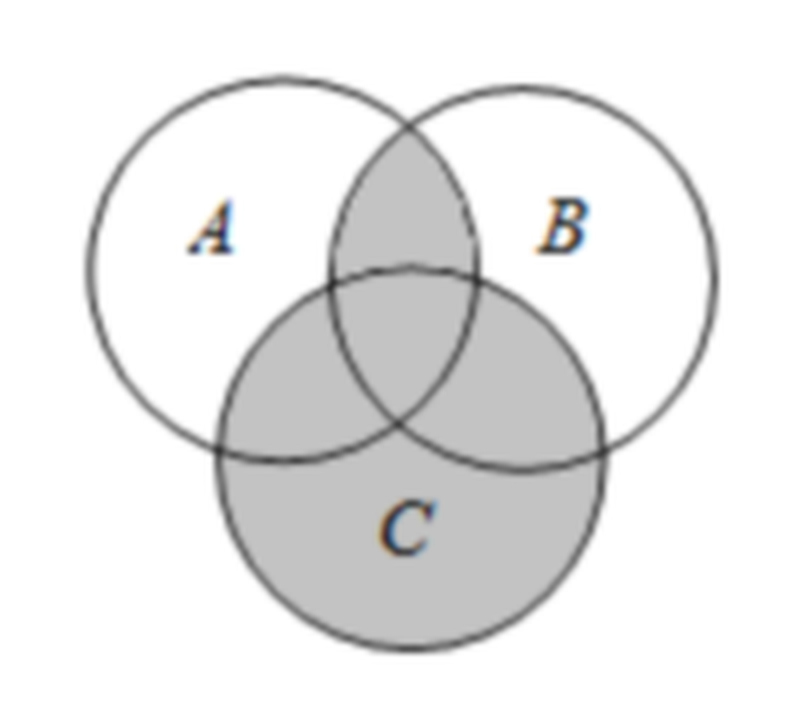
\includegraphics[width=0.30\textwidth]{figures/venn_ABcap_plus_C.png}
\end{center}

\keepwithprev
A. $(A\cup C)\cap(B\cup C)$\qquad B. $(A\cup B)\cap(A\cup C)$

C. $(A\cup B)\cap(B\cup C)$\qquad D. $(A\cup B)\cap C$

\ans{$A$}

\item 设 $f(x)=(x^2-6x+c_1)(x^2-6x+c_2)$，其中 $c_1\geqslant c_2$，集合

$M=\{x\mid f(x)=0\}=\{x_1,x_2,x_3\}\sub\Z$，则下列命题中不正确的是\mbox{（\quad）}

\keepwithprev
A. $3\in M$\qquad B. $c_2$ 可能为 $-16$

C. $c_1$ 可能为 $8$\qquad D. $M$ 中所有元素的和一定为 $9$

\ans{$C$}

\ifanswer
\solbegin
\step{若 $c_1$ 为 $8$，则 $c_2=9$，与 $c_1\geqslant c_2$ 矛盾，故选 $C$.}
\solend

\fi

\item 非空集合 $A$ 具有如下性质：①若 $x$、$y\in A$，则 $\dfrac{x}{y}\in A$；②若 $x$、$y\in A$，
则 $x+y\in A$；

由此可知：下列判断中，错误的是\mbox{（\quad）}

\keepwithprev
A. $-1\notin A$\qquad B. $\dfrac{2025}{2026}\in A$

C. 若 $x$、$y\in A$，则 $xy\in A$\qquad D. 若 $x$、$y\in A$，则 $x-y\in A$

\ans{$D$}

\ifanswer
\solbegin
\step{由题意得 $0\notin A$，$1\in A$，}
\step{对于 $A$，假设 $-1\in A$，则 $-1+1=0\in A$，矛盾，所以 $-1\notin A$，故 $A$ 正确；}
\step{对于 $B$，由 $1\in A$，得 $1+1=2\in A$，$2+1=3\in A$，$\cdots$，$2025\in A$，$2026\in A$，}
\step{所以 $\dfrac{2025}{2026}\in A$，故 $B$ 正确；}
\step{对于 $C$，因为 $1\in A$，$x\in A$，所以 $\dfrac1x\in A$，又因为 $y\in A$，
所以 $\dfrac{y}{\frac1x}=xy\in A$，}
\step{故 $C$ 正确；}
\step{对于 $D$，因为 $1\in A$，$2\in A$，若 $x=1$，$y=2$，则 $x-y=-1\notin A$，故 $D$ 错误.}
\step{故选 $D$.}
\solend

\fi

\end{enumerate}

\bigsec{三、解答题}

\begin{enumerate}
\setcounter{enumi}{13}

% 注：原卷本题题干把「$=0$」印在右花括号之外（$A=\{x\mid x^2-mx+4m-16\}=0$），
%     而其自己的【解析】印在括号之内（$A=\{x\mid x^2-mx+4m-16=0\}$）——原卷前后不一致，
%     本稿按解析与题目本意把 $=0$ 排在括号内，见文件头「排版差异」⑧。
\item 已知集合 $A=\{x\mid x^2-mx+4m-16=0\}$，$B=\{x\mid 1<x<4,x\in\N\}$，
$C=\{x\mid ax+2>0\}$，若 $A\cap B\neq\varnothing$，$A\cap C=\varnothing$，求实数 $m$ 的值以及
相应实数 $a$ 的取值范围.

\ifanswer
\solbegin
\step{集合 $A=\{x\mid x^2-mx+4m-16=0\}$，由 $\Delta=(-m)^2-4(4m-16)=(m-8)^2\geqslant0$，}
\step{所以当 $m=8$ 时，集合 $A=\{4\}$，当 $m\neq8$ 时，集合
$A=\left\{\dfrac{m-|m-8|}{2},\dfrac{m+|m-8|}{2}\right\}$，}
\step{集合 $B=\{x\mid 1<x<4,x\in\N\}$，得集合 $B=\{2,3\}$.}
\step{集合 $C=\{x\mid ax+2>0\}$，当 $a=0$ 时，集合 $C=\{x\mid x\in\R\}$，}
\step{当 $a<0$ 时，集合 $C=\left\{x\mid x<\dfrac2a\right\}$，当 $a>0$ 时，集合
$C=\left\{x\mid x>\dfrac2a\right\}$，}
\step{由 $A\cap B$ 非空得，$m=6$ 时，集合 $A=\{2,4\}$，$m=7$ 时，集合 $A=\{3,4\}$.}
\step{由 $A\cap C=\varnothing$，得 $m=6$ 或 $m=7$ 时，$a<0$ 或 $0<a<\dfrac12$ 符合要求.}
\solend

\fi

\ansspace[9]

\item 已知 $a>b>c$，$a+b+c=0$，方程 $ax^2+bx+c=0$ 的两个实根为 $x_1$、$x_2$.

\begin{enumerate}[label=(\arabic*)]
\item 证明：$-\dfrac12<\dfrac ba<1$；
% 注：此小问前加了 4pt 间距——不加时紧凑版该行的 $x_1^2$ 上标与下标恰好同箱，
%     pdftotext 抽正文会把上标当重影丢掉，make check 的正文指纹就对不上（纯抽取抖动，
%     版面与内容无差别，见 2026-09-20 入库注）。
\vspace{4pt}
\item 若 $x_1^2+x_1x_2+x_2^2=1$，求 $x_1^2-x_1x_2+x_2^2$.
\end{enumerate}

\ifanswer
\solbegin
\stepm{(1)}{因为 $a>b>c$，$a+b+c=0$，所以 $a>0$，$c<0$，$c=-a-b$，}
\step{由 $a>b$ 得 $\dfrac ba<1$ ①，由 $b>c$ 得 $b>-a-b$，即 $2b>-a$，即 $\dfrac ba>-\dfrac12$ ②，}
\step{由①②得 $-\dfrac12<\dfrac ba<1$；}
\stepm{(2)}{若 $x_1^2+x_1x_2+x_2^2=1$，则 $(x_1+x_2)^2-x_1x_2=1$，}
% 注：本行的连等式与原卷自己的结论对不上（照抄原卷、未改）——原卷印作
%     (b/a)²-b/a+1=1，则解出的应是 0 或 1；按 c=-a-b 应为 (b/a)²+b/a+1=1，
%     解得 0 或 -1（-1 因 c<0 舍去），恰与下一行「0 或 -1（舍去）」吻合。
%     详见文件头「原卷存疑」①。
\step{则 $\left(\dfrac ba\right)^2-\dfrac ca=\dfrac{b^2-ac}{a^2}
=\left(\dfrac ba\right)^2-\dfrac ba+1=1$，解得 $\dfrac ba=0$ 或 $-1$（舍去），}
\step{故 $\dfrac ba=0$，$\dfrac ca=-1$，}
\step{所以 $x_1^2-x_1x_2+x_2^2=(x_1+x_2)^2-3x_1x_2=\left(\dfrac ba\right)^2-3\times\dfrac ca=3$.}
\solend

\fi

\ansspace[6]

\item 已知方程 $x^2+px+q=0$ 与方程 $x^2+(p-3)x+2q+1=0$ 分别都有两个不相等的实根，若
他们的解集分别为 $A$、$B$，且 $A\cup B=\{1,2,5\}$，求 $p$、$q$、$A$、$B$.

\ifanswer
\solbegin
\step{两方程分别有两个不相等的实数根，而根的并集只有 $3$ 个元素，}
\step{则两方程有一公共根. 分类讨论：}
\stepm{（1）}{公共根为 $1$ 时，$x=1$ 分别代入两方程：}
\step{$\begin{cases}p+q+1=0\\ p-3+2q+1+1=0\end{cases}$，解得 $p=-3$，$q=2$，}
\step{两方程变为 $x^2-3x+2=0$，解得 $x=1$ 或 $x=2$，}
\step{$x^2-6x+5=0$ 解得 $x=1$ 或 $x=5$，满足题意.}
\stepm{（2）}{公共根为 $2$ 时，$x=2$ 分别代入两方程：}
\step{$\begin{cases}4+2p+q=0\\ 4+2p-6+2q+1=0\end{cases}$，解得 $p=-\dfrac92$，$q=5$，}
\step{第一个方程变为 $2x^2-9x+10=0$，解得 $x=2$ 或 $x=\dfrac52$，不满足题意，舍去.}
\stepm{（3）}{公共根为 $5$ 时，$x=5$ 分别代入两方程：}
\step{$\begin{cases}25+5p+q=0\\ 25+5p-15+2q+1=0\end{cases}$，解得 $p=-\dfrac{39}{5}$，$q=14$，}
\step{第一个方程变为 $5x^2-39x+70=0$，解得 $x=5$ 或 $x=\dfrac{14}{5}$，不满足题意，舍去.}
\step{综上，$p=-3$，$q=2$，$A=\{1,2\}$，$B=\{1,5\}$.}
\solend

\fi

\ansspace[8]

\item 对于集合 $A=\{a_1,a_2,\cdots,a_n\}(n\in\Z,n\geqslant3)$，其中每个元素均为正整数，如果
任意去掉其
中一个元素 $a_i(i=1,2,3\cdots,n)$ 之后，剩余的所有元素组成集合 $A_i(i=1,2,\cdots,n)$，并且
$A_i$ 都能分为两个集合 $B$ 和 $C$，满足 $B\cap C=\varnothing,B\cup C=A_i$，其中 $B$ 和 $C$
的所有元素之和相
等，就称集合 $A$ 为“可分集合”.

\begin{enumerate}[label=(\arabic*)]
\item 判断集合 $\{1,3,5,7,9,11,13\}$ 是否是“可分集合”（不必写过程）；
\item 用反证法证明：五个元素的集合 $A=\{a_1,a_2,a_3,a_4,a_5\}$ 一定不是“可分集合”；
\item 已知集合 $A=\{a_1,a_2,\cdots,a_n\}(n\in\Z,n\geqslant3)$ 是“可分集合”，求 $n$ 的最小值.
\end{enumerate}

\ifanswer
\solbegin
\stepm{(1)}{集合 $\{1,3,5,7,9,11,13\}$ 是“可分集合”；}
\stepm{(2)}{不妨设 $a_1<a_2<a_3<a_4<a_5$，}
\step{若去掉的元素为 $a_2$，将集合 $\{a_1,a_3,a_4,a_5\}$ 分成两个交集为空集的子集，}
\step{且两个子集元素之和相等，则有 $a_1+a_5=a_3+a_4$ ①，或者 $a_5=a_1+a_3+a_4$ ②；}
\step{若去掉的元素为 $a_1$，将集合 $\{a_2,a_3,a_4,a_5\}$ 分成两个交集为空集的子集，}
\step{且两个子集元素之和相等，则有 $a_2+a_5=a_3+a_4$ ③，或者 $a_5=a_2+a_3+a_4$ ④.}
\step{由①、③，得 $a_1=a_2$，矛盾；由①、④，得 $a_1=-a_2$，矛盾；}
\step{由②、③，得 $a_1=-a_2$，矛盾；由②、④，得 $a_1=a_2$ 矛盾.}
\step{因此当 $n=5$ 时，集合一定不是“可分集合”；}
\stepm{(3)}{①设集合 $A=\{a_1,a_2,\cdots,a_n\}$ 的所有元素之和为 $M$.}
\step{由题意得 $M-a_i(i=1,2,\cdots,n)$ 均为偶数，}
\step{因此 $a_i(i=1,2,\cdots,n)$ 均为奇数或偶数.}
\step{如果 $M$ 为奇数，则 $a_i(i=1,2,\cdots,n)$ 也均为奇数，}
\step{由于 $M=a_1+a_2+\cdots+a_n$，所以 $n$ 为奇数.}
\step{如果 $M$ 为偶数，则 $M-a_i(i=1,2,\cdots,n)$ 均为偶数，此时设 $a_i=2b_i$，}
\step{则 $\{b_1,b_2,\cdots,b_n\}$ 也是“可分集合”.}
\step{重复上述操作有限次，便可得各项均为奇数的“可分集合”，}
\step{此时各项之和也为奇数，则集合 $A$ 中元素个数 $n$ 为奇数.}
\step{综上所述，集合 $A$ 中元素个数为奇数.}
\step{②当 $n=3$ 时，显然任意集合 $\{a_1,a_2,a_3\}$ 不是“可分集合”.}
\step{当 $n=5$ 时，第（2）问已经证明不是“可分集合”.}
\step{当 $n=7$ 时，集合 $A=\{1,3,5,7,9,11,13\}$，}
\step{因为 $3+5+7+9=11+13$，$1+9+13=5+7+11$，$9+13=1+3+7+11$，}
\step{$1+3+5+11=7+13$，$1+9+11=3+5+13$，$3+7+9=1+5+13$，}
\step{$1+3+5+9=7+11$，则集合 $A$ 是“可分集合”，}
\step{所以集合 $A$ 中元素个数 $n$ 的最小值是 $7$.}
\solend

\fi

\ansspace*[10]

\end{enumerate}

\end{document}
"
% 紧凑版：xelatex "\def\iscompact{1}% 高一24_复旦附中_周末作业3.tex
%   —— 高一上数学「2026-2027 年复旦附中高一上周末作业 3」（试卷版/答案版）
% 试卷版：xelatex 高一24_复旦附中_周末作业3.tex
% 答案版：xelatex "\def\isanswer{1}\input{高一24_复旦附中_周末作业3.tex}"
% 紧凑版：xelatex "\def\iscompact{1}\input{高一24_复旦附中_周末作业3.tex}"
%
% 原始材料是微信公众号图文（公众号「魔都数学加油站」连载「27学年高一 24」，2026-09-19 发布，
% 原文标题「27学年高一24——2026-2027年上海市复旦附中高一上周末作业3集合与逻辑、等式的性质」），
% 正文为 7 张 PNG 页（1080×1527，各页同尺寸）。原文本身就是一份**讲评版**——题目下方直接印出
% 【答案】或【解析】。试题文字、答案与解析均照原卷录入，未改内容。
% 卷面上的粉色斜水印「魔都数学加油站」属水印，未录入。
%
% 卷首标题：原卷印作「2026-2027 年复旦附中高一上周末作业 3」（公众号标题里有「上海市」三字，
% 卷面标题行没有，本稿照卷面），年份区间按全稿惯例排 en dash，前缀照原卷保留「年」。
%
% 与原卷的排版差异（均已在 README「说明」中交代）：
%   ① 原文自**第 3 题**起（第 1、2 题未在该文中发布），故本稿题号亦自 3 起；
%   ② 原卷本就印有「一、填空题」「二、选择题」「三、解答题」三节标题，本稿照原卷分节，
%      只把标题改排成全稿统一的「大节标题」样式；
%   ③ 原卷第 11 题的答案「A」直接印在题干末尾的括号内，第 12、13 题的括号空着、答案写在
%      解析末句「故选 C／D」里，本稿统一改为试卷版隐去、答案版以 \ans{} 给出（第 12、13 题
%      另附【解析】），使两版彻底分离；
%   ④ 原卷的集合／数集符号正体与粗体混用（第 8 题题干的 $\mathbf{R}$、第 9 题题干的
%      $\mathbf{N}$、第 12 题题干的 $\mathbf{Z}$ 为粗体，第 14 题解析的 $N$、$R$ 为斜体），
%      本稿按全稿惯例统一写作 $\R$、$\N$、$\Z$；
%   ⑤ 原卷填空的横线约两个字宽，本稿按全稿惯例统一排 \blankline[4.4em]；
%   ⑥ 第 11 题的 Venn 图原卷印在上一页末尾（第 10 题解析右侧、「二、选择题」标题旁），
%      本稿移至第 11 题题干之后；图取原卷截图、4× LANCZOS 放大
%      （figures/venn_ABcap_plus_C.png，阴影为 $A\cap B$ 的交与整个 $C$，即 $(A\cap B)\cup C$）；
%   ⑦ 原卷自印副标题「集合与逻辑、等式的性质」，本稿照录（与 高一14 同例，未改用惯例副标题）；
%   ⑧ 第 14 题题干原卷把「$=0$」印在右花括号**之外**（作
%      $A=\{x\mid x^2-mx+4m-16\}=0$），而它**自己的【解析】却印在括号之内**
%      （作 $A=\{x\mid x^2-mx+4m-16=0\}$）——原卷前后不一致；按原卷解析与题目本意，
%      本稿题干的 $=0$ 排在括号**之内**（与 高一b 第 13 题「原卷漏排 $A=$，本稿补上」同例）。
%
% 原卷存疑一处（已放大到能看清字形后核对，无法确证原意，本稿照抄原卷、未改）：
%   ① 第 15(2)【解析】的连等式印作
%      $\left(\frac ba\right)^2-\frac ca=\frac{b^2-ac}{a^2}=\left(\frac ba\right)^2-\frac ba+1=1$，
%      解得 $\frac ba=0$ 或 $-1$（舍去）——但由 $c=-a-b$ 应得 $\frac{b^2-ac}{a^2}
%      =\left(\frac ba\right)^2+\frac ba+1$（原卷把「$+\frac ba$」印成了「$-\frac ba$」）：
%      按原卷那行解出的是 $0$ 或 $1$，与其自己的结论「$0$ 或 $-1$」对不上；而按
%      $+\frac ba$ 解恰得 $0$ 或 $-1$（$-1$ 因 $c<0$ 舍去），与后文吻合。原卷显系笔误，
%      本稿照抄原卷（见源码中该处上方注释）。

\documentclass[a4paper,11pt]{article}
\usepackage{common}

\begin{document}

\examtitlest[3]{2026--2027 年复旦附中高一上周末作业 3}{集合与逻辑、等式的性质}

\bigsec{一、填空题}

\begin{enumerate}
\setcounter{enumi}{2}

\item 设 $M=\{x\mid y^2=x+2\}$，$N=\{x\mid y^2=-2x+8\}$，则 $M\cap N=$ \blankline[4.4em].

\ifanswer
\solbegin
\step{$M=[-2,+\infty)$，$N=(-\infty,4]$，则 $M\cap N=[-2,4]$.}
\solend

\fi

\item 若“$x\geqslant a$”是“$|x|\leqslant2$”的必要条件，则实数 $a$ 的取值集合是 \blankline[4.4em].

\ans{$(-\infty,-2]$}

\item 某校一年级的 $200$ 人中，爱好数学的有 $95$ 人，爱好体育的有 $156$ 人，则数学体育都爱好
的至少有 \blankline[4.4em] 人.

\ifanswer
\solbegin
\step{数学体育都爱好的至少有 $95+156-200=51$ 人.}
\solend

\fi

\item 已知 $x$ 为实数，且 $x^2+\dfrac{1}{x^2}=3$，则 $x^3+\dfrac{1}{x^3}$ 的值是 \blankline[4.4em].

\ifanswer
\solbegin
\step{因为 $x^2+\dfrac{1}{x^2}=\left(x+\dfrac1x\right)^2-2=3$，所以 $x+\dfrac1x=\pm\sqrt5$，}
\step{所以 $x^3+\dfrac{1}{x^3}=\left(x+\dfrac1x\right)\left(x^2-1+\dfrac{1}{x^2}\right)=\pm2\sqrt5$.}
\solend

\fi

\item 非空集合 $A=\{x\mid a+1\leqslant x<2a-1\}$，$B=\{x\mid-2\leqslant x\leqslant5\}$，
若 $A\sub(A\cap B)$，则 $a$ 的取值范围是 \blankline[4.4em].

\ifanswer
\solbegin
\step{当 $a+1<2a-1$，即 $a>2$ 时，$A\neq\varnothing$，由 $A\sub(A\cap B)$ 得 $A\sub B$，}
\step{得 $\begin{cases}a+1\geqslant-2\\ 2a-1\leqslant5\end{cases}$，解得 $-3\leqslant a\leqslant3$，所以 $2<a\leqslant3$.}
\solend

\fi

\item 已知集合 $\{x\mid(x-1)(x^2-x+a)=0,x\in\R\}$ 中的所有元素之和为 $1$，则实数 $a$ 的取值范
围是 \blankline[4.4em].

\ifanswer
\solbegin
\step{令 $x-1=0$，得 $x=1$，}
\stepm{①}{若 $x^2-x+a=0$ 无实数根，则 $\Delta=1-4a<0$，解得 $a>\dfrac14$，}
\step{此时集合只有元素 $1$，符合题意；}
\stepm{②}{若 $x^2-x+a=0$ 有两个相等的实数根，则 $\Delta=1-4a=0$，解得 $a=\dfrac14$，}
\step{此时方程为 $x^2-x+\dfrac14=0$，解得 $x=\dfrac12$，此时集合为 $\left\{1,\dfrac12\right\}$，不合题意；}
\stepm{③}{若 $x^2-x+a=0$ 有两个不相等的实数根，则 $\Delta=1-4a>0$，解得 $a<\dfrac14$，}
\step{设方程 $x^2-x+a=0$ 的两个实根分别为 $x_1,x_2$，则 $x_1+x_2=1$，}
\step{若 $x_1\neq1,x_2\neq1$，则集合为 $\{1,x_1,x_2\}$，不合题意，}
\step{若 $x_1=1$，则 $x_2=0$，此时集合为 $\{1,0\}$，符合题意，所以 $a=x_1x_2=0$，}
\step{综上所述，实数 $a$ 的取值范围是 $\{0\}\cup\left(\dfrac14,+\infty\right)$.}
\solend

\fi

\item 集合 $A=\{m\mid m=2k,k\in\N,1\leqslant k\leqslant50\}$，
$B=\{n\mid n=i+j,i<j,i\in A,j\in A\}$，则 $B$ 中元素的个数是 \blankline[4.4em].

\ifanswer
\solbegin
\step{$B$ 中最小元素是 $6$，最大元素是 $198$，则 $B$ 中元素的个数是 $\dfrac{198-6}{2}+1=97$.}
\solend

\fi

\item 关于 $(x,y,z)$ 的方程组
$\begin{cases}x^2+y^2+25z^2=6zx+8yz\\ 3x^2+2y^2+z^2=240\end{cases}$ 的解集为 \blankline[4.4em].

\ifanswer
\solbegin
\step{由上式得 $(x^2-6xz+9z^2)+(y^2-8yz+16z^2)=0$，}
\step{则 $(x-3z)^2+(y-4z)^2=0$，}
\step{所以 $(x,y,z)=(3t,4t,t)$，$t$ 为实数，代入下式中 $27\cdot t^2+32t^2+t^2=60t^2=240$，}
\step{则 $t^2=4$，$t=\pm2$，所以 $(x,y,z)=(6,8,2),(-6,-8,-2)$.}
\solend

\fi

\end{enumerate}

\bigsec{二、选择题}

\begin{enumerate}
\setcounter{enumi}{10}

\item 下列表示图形中的阴影部分的是\mbox{（\quad）}

\begin{center}
% 图取原卷截图、4× LANCZOS 放大（原卷把图印在上一页末尾，本稿移至此处，见文件头⑥）。
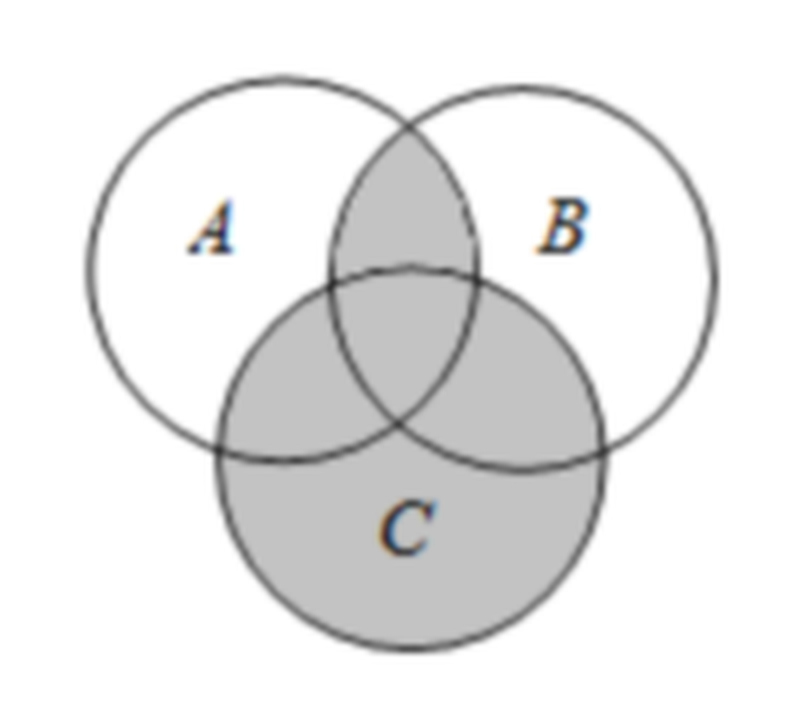
\includegraphics[width=0.30\textwidth]{figures/venn_ABcap_plus_C.png}
\end{center}

\keepwithprev
A. $(A\cup C)\cap(B\cup C)$\qquad B. $(A\cup B)\cap(A\cup C)$

C. $(A\cup B)\cap(B\cup C)$\qquad D. $(A\cup B)\cap C$

\ans{$A$}

\item 设 $f(x)=(x^2-6x+c_1)(x^2-6x+c_2)$，其中 $c_1\geqslant c_2$，集合

$M=\{x\mid f(x)=0\}=\{x_1,x_2,x_3\}\sub\Z$，则下列命题中不正确的是\mbox{（\quad）}

\keepwithprev
A. $3\in M$\qquad B. $c_2$ 可能为 $-16$

C. $c_1$ 可能为 $8$\qquad D. $M$ 中所有元素的和一定为 $9$

\ans{$C$}

\ifanswer
\solbegin
\step{若 $c_1$ 为 $8$，则 $c_2=9$，与 $c_1\geqslant c_2$ 矛盾，故选 $C$.}
\solend

\fi

\item 非空集合 $A$ 具有如下性质：①若 $x$、$y\in A$，则 $\dfrac{x}{y}\in A$；②若 $x$、$y\in A$，
则 $x+y\in A$；

由此可知：下列判断中，错误的是\mbox{（\quad）}

\keepwithprev
A. $-1\notin A$\qquad B. $\dfrac{2025}{2026}\in A$

C. 若 $x$、$y\in A$，则 $xy\in A$\qquad D. 若 $x$、$y\in A$，则 $x-y\in A$

\ans{$D$}

\ifanswer
\solbegin
\step{由题意得 $0\notin A$，$1\in A$，}
\step{对于 $A$，假设 $-1\in A$，则 $-1+1=0\in A$，矛盾，所以 $-1\notin A$，故 $A$ 正确；}
\step{对于 $B$，由 $1\in A$，得 $1+1=2\in A$，$2+1=3\in A$，$\cdots$，$2025\in A$，$2026\in A$，}
\step{所以 $\dfrac{2025}{2026}\in A$，故 $B$ 正确；}
\step{对于 $C$，因为 $1\in A$，$x\in A$，所以 $\dfrac1x\in A$，又因为 $y\in A$，
所以 $\dfrac{y}{\frac1x}=xy\in A$，}
\step{故 $C$ 正确；}
\step{对于 $D$，因为 $1\in A$，$2\in A$，若 $x=1$，$y=2$，则 $x-y=-1\notin A$，故 $D$ 错误.}
\step{故选 $D$.}
\solend

\fi

\end{enumerate}

\bigsec{三、解答题}

\begin{enumerate}
\setcounter{enumi}{13}

% 注：原卷本题题干把「$=0$」印在右花括号之外（$A=\{x\mid x^2-mx+4m-16\}=0$），
%     而其自己的【解析】印在括号之内（$A=\{x\mid x^2-mx+4m-16=0\}$）——原卷前后不一致，
%     本稿按解析与题目本意把 $=0$ 排在括号内，见文件头「排版差异」⑧。
\item 已知集合 $A=\{x\mid x^2-mx+4m-16=0\}$，$B=\{x\mid 1<x<4,x\in\N\}$，
$C=\{x\mid ax+2>0\}$，若 $A\cap B\neq\varnothing$，$A\cap C=\varnothing$，求实数 $m$ 的值以及
相应实数 $a$ 的取值范围.

\ifanswer
\solbegin
\step{集合 $A=\{x\mid x^2-mx+4m-16=0\}$，由 $\Delta=(-m)^2-4(4m-16)=(m-8)^2\geqslant0$，}
\step{所以当 $m=8$ 时，集合 $A=\{4\}$，当 $m\neq8$ 时，集合
$A=\left\{\dfrac{m-|m-8|}{2},\dfrac{m+|m-8|}{2}\right\}$，}
\step{集合 $B=\{x\mid 1<x<4,x\in\N\}$，得集合 $B=\{2,3\}$.}
\step{集合 $C=\{x\mid ax+2>0\}$，当 $a=0$ 时，集合 $C=\{x\mid x\in\R\}$，}
\step{当 $a<0$ 时，集合 $C=\left\{x\mid x<\dfrac2a\right\}$，当 $a>0$ 时，集合
$C=\left\{x\mid x>\dfrac2a\right\}$，}
\step{由 $A\cap B$ 非空得，$m=6$ 时，集合 $A=\{2,4\}$，$m=7$ 时，集合 $A=\{3,4\}$.}
\step{由 $A\cap C=\varnothing$，得 $m=6$ 或 $m=7$ 时，$a<0$ 或 $0<a<\dfrac12$ 符合要求.}
\solend

\fi

\ansspace[9]

\item 已知 $a>b>c$，$a+b+c=0$，方程 $ax^2+bx+c=0$ 的两个实根为 $x_1$、$x_2$.

\begin{enumerate}[label=(\arabic*)]
\item 证明：$-\dfrac12<\dfrac ba<1$；
% 注：此小问前加了 4pt 间距——不加时紧凑版该行的 $x_1^2$ 上标与下标恰好同箱，
%     pdftotext 抽正文会把上标当重影丢掉，make check 的正文指纹就对不上（纯抽取抖动，
%     版面与内容无差别，见 2026-09-20 入库注）。
\vspace{4pt}
\item 若 $x_1^2+x_1x_2+x_2^2=1$，求 $x_1^2-x_1x_2+x_2^2$.
\end{enumerate}

\ifanswer
\solbegin
\stepm{(1)}{因为 $a>b>c$，$a+b+c=0$，所以 $a>0$，$c<0$，$c=-a-b$，}
\step{由 $a>b$ 得 $\dfrac ba<1$ ①，由 $b>c$ 得 $b>-a-b$，即 $2b>-a$，即 $\dfrac ba>-\dfrac12$ ②，}
\step{由①②得 $-\dfrac12<\dfrac ba<1$；}
\stepm{(2)}{若 $x_1^2+x_1x_2+x_2^2=1$，则 $(x_1+x_2)^2-x_1x_2=1$，}
% 注：本行的连等式与原卷自己的结论对不上（照抄原卷、未改）——原卷印作
%     (b/a)²-b/a+1=1，则解出的应是 0 或 1；按 c=-a-b 应为 (b/a)²+b/a+1=1，
%     解得 0 或 -1（-1 因 c<0 舍去），恰与下一行「0 或 -1（舍去）」吻合。
%     详见文件头「原卷存疑」①。
\step{则 $\left(\dfrac ba\right)^2-\dfrac ca=\dfrac{b^2-ac}{a^2}
=\left(\dfrac ba\right)^2-\dfrac ba+1=1$，解得 $\dfrac ba=0$ 或 $-1$（舍去），}
\step{故 $\dfrac ba=0$，$\dfrac ca=-1$，}
\step{所以 $x_1^2-x_1x_2+x_2^2=(x_1+x_2)^2-3x_1x_2=\left(\dfrac ba\right)^2-3\times\dfrac ca=3$.}
\solend

\fi

\ansspace[6]

\item 已知方程 $x^2+px+q=0$ 与方程 $x^2+(p-3)x+2q+1=0$ 分别都有两个不相等的实根，若
他们的解集分别为 $A$、$B$，且 $A\cup B=\{1,2,5\}$，求 $p$、$q$、$A$、$B$.

\ifanswer
\solbegin
\step{两方程分别有两个不相等的实数根，而根的并集只有 $3$ 个元素，}
\step{则两方程有一公共根. 分类讨论：}
\stepm{（1）}{公共根为 $1$ 时，$x=1$ 分别代入两方程：}
\step{$\begin{cases}p+q+1=0\\ p-3+2q+1+1=0\end{cases}$，解得 $p=-3$，$q=2$，}
\step{两方程变为 $x^2-3x+2=0$，解得 $x=1$ 或 $x=2$，}
\step{$x^2-6x+5=0$ 解得 $x=1$ 或 $x=5$，满足题意.}
\stepm{（2）}{公共根为 $2$ 时，$x=2$ 分别代入两方程：}
\step{$\begin{cases}4+2p+q=0\\ 4+2p-6+2q+1=0\end{cases}$，解得 $p=-\dfrac92$，$q=5$，}
\step{第一个方程变为 $2x^2-9x+10=0$，解得 $x=2$ 或 $x=\dfrac52$，不满足题意，舍去.}
\stepm{（3）}{公共根为 $5$ 时，$x=5$ 分别代入两方程：}
\step{$\begin{cases}25+5p+q=0\\ 25+5p-15+2q+1=0\end{cases}$，解得 $p=-\dfrac{39}{5}$，$q=14$，}
\step{第一个方程变为 $5x^2-39x+70=0$，解得 $x=5$ 或 $x=\dfrac{14}{5}$，不满足题意，舍去.}
\step{综上，$p=-3$，$q=2$，$A=\{1,2\}$，$B=\{1,5\}$.}
\solend

\fi

\ansspace[8]

\item 对于集合 $A=\{a_1,a_2,\cdots,a_n\}(n\in\Z,n\geqslant3)$，其中每个元素均为正整数，如果
任意去掉其
中一个元素 $a_i(i=1,2,3\cdots,n)$ 之后，剩余的所有元素组成集合 $A_i(i=1,2,\cdots,n)$，并且
$A_i$ 都能分为两个集合 $B$ 和 $C$，满足 $B\cap C=\varnothing,B\cup C=A_i$，其中 $B$ 和 $C$
的所有元素之和相
等，就称集合 $A$ 为“可分集合”.

\begin{enumerate}[label=(\arabic*)]
\item 判断集合 $\{1,3,5,7,9,11,13\}$ 是否是“可分集合”（不必写过程）；
\item 用反证法证明：五个元素的集合 $A=\{a_1,a_2,a_3,a_4,a_5\}$ 一定不是“可分集合”；
\item 已知集合 $A=\{a_1,a_2,\cdots,a_n\}(n\in\Z,n\geqslant3)$ 是“可分集合”，求 $n$ 的最小值.
\end{enumerate}

\ifanswer
\solbegin
\stepm{(1)}{集合 $\{1,3,5,7,9,11,13\}$ 是“可分集合”；}
\stepm{(2)}{不妨设 $a_1<a_2<a_3<a_4<a_5$，}
\step{若去掉的元素为 $a_2$，将集合 $\{a_1,a_3,a_4,a_5\}$ 分成两个交集为空集的子集，}
\step{且两个子集元素之和相等，则有 $a_1+a_5=a_3+a_4$ ①，或者 $a_5=a_1+a_3+a_4$ ②；}
\step{若去掉的元素为 $a_1$，将集合 $\{a_2,a_3,a_4,a_5\}$ 分成两个交集为空集的子集，}
\step{且两个子集元素之和相等，则有 $a_2+a_5=a_3+a_4$ ③，或者 $a_5=a_2+a_3+a_4$ ④.}
\step{由①、③，得 $a_1=a_2$，矛盾；由①、④，得 $a_1=-a_2$，矛盾；}
\step{由②、③，得 $a_1=-a_2$，矛盾；由②、④，得 $a_1=a_2$ 矛盾.}
\step{因此当 $n=5$ 时，集合一定不是“可分集合”；}
\stepm{(3)}{①设集合 $A=\{a_1,a_2,\cdots,a_n\}$ 的所有元素之和为 $M$.}
\step{由题意得 $M-a_i(i=1,2,\cdots,n)$ 均为偶数，}
\step{因此 $a_i(i=1,2,\cdots,n)$ 均为奇数或偶数.}
\step{如果 $M$ 为奇数，则 $a_i(i=1,2,\cdots,n)$ 也均为奇数，}
\step{由于 $M=a_1+a_2+\cdots+a_n$，所以 $n$ 为奇数.}
\step{如果 $M$ 为偶数，则 $M-a_i(i=1,2,\cdots,n)$ 均为偶数，此时设 $a_i=2b_i$，}
\step{则 $\{b_1,b_2,\cdots,b_n\}$ 也是“可分集合”.}
\step{重复上述操作有限次，便可得各项均为奇数的“可分集合”，}
\step{此时各项之和也为奇数，则集合 $A$ 中元素个数 $n$ 为奇数.}
\step{综上所述，集合 $A$ 中元素个数为奇数.}
\step{②当 $n=3$ 时，显然任意集合 $\{a_1,a_2,a_3\}$ 不是“可分集合”.}
\step{当 $n=5$ 时，第（2）问已经证明不是“可分集合”.}
\step{当 $n=7$ 时，集合 $A=\{1,3,5,7,9,11,13\}$，}
\step{因为 $3+5+7+9=11+13$，$1+9+13=5+7+11$，$9+13=1+3+7+11$，}
\step{$1+3+5+11=7+13$，$1+9+11=3+5+13$，$3+7+9=1+5+13$，}
\step{$1+3+5+9=7+11$，则集合 $A$ 是“可分集合”，}
\step{所以集合 $A$ 中元素个数 $n$ 的最小值是 $7$.}
\solend

\fi

\ansspace*[10]

\end{enumerate}

\end{document}
"
%
% 原始材料是微信公众号图文（公众号「魔都数学加油站」连载「27学年高一 24」，2026-09-19 发布，
% 原文标题「27学年高一24——2026-2027年上海市复旦附中高一上周末作业3集合与逻辑、等式的性质」），
% 正文为 7 张 PNG 页（1080×1527，各页同尺寸）。原文本身就是一份**讲评版**——题目下方直接印出
% 【答案】或【解析】。试题文字、答案与解析均照原卷录入，未改内容。
% 卷面上的粉色斜水印「魔都数学加油站」属水印，未录入。
%
% 卷首标题：原卷印作「2026-2027 年复旦附中高一上周末作业 3」（公众号标题里有「上海市」三字，
% 卷面标题行没有，本稿照卷面），年份区间按全稿惯例排 en dash，前缀照原卷保留「年」。
%
% 与原卷的排版差异（均已在 README「说明」中交代）：
%   ① 原文自**第 3 题**起（第 1、2 题未在该文中发布），故本稿题号亦自 3 起；
%   ② 原卷本就印有「一、填空题」「二、选择题」「三、解答题」三节标题，本稿照原卷分节，
%      只把标题改排成全稿统一的「大节标题」样式；
%   ③ 原卷第 11 题的答案「A」直接印在题干末尾的括号内，第 12、13 题的括号空着、答案写在
%      解析末句「故选 C／D」里，本稿统一改为试卷版隐去、答案版以 \ans{} 给出（第 12、13 题
%      另附【解析】），使两版彻底分离；
%   ④ 原卷的集合／数集符号正体与粗体混用（第 8 题题干的 $\mathbf{R}$、第 9 题题干的
%      $\mathbf{N}$、第 12 题题干的 $\mathbf{Z}$ 为粗体，第 14 题解析的 $N$、$R$ 为斜体），
%      本稿按全稿惯例统一写作 $\R$、$\N$、$\Z$；
%   ⑤ 原卷填空的横线约两个字宽，本稿按全稿惯例统一排 \blankline[4.4em]；
%   ⑥ 第 11 题的 Venn 图原卷印在上一页末尾（第 10 题解析右侧、「二、选择题」标题旁），
%      本稿移至第 11 题题干之后；图取原卷截图、4× LANCZOS 放大
%      （figures/venn_ABcap_plus_C.png，阴影为 $A\cap B$ 的交与整个 $C$，即 $(A\cap B)\cup C$）；
%   ⑦ 原卷自印副标题「集合与逻辑、等式的性质」，本稿照录（与 高一14 同例，未改用惯例副标题）；
%   ⑧ 第 14 题题干原卷把「$=0$」印在右花括号**之外**（作
%      $A=\{x\mid x^2-mx+4m-16\}=0$），而它**自己的【解析】却印在括号之内**
%      （作 $A=\{x\mid x^2-mx+4m-16=0\}$）——原卷前后不一致；按原卷解析与题目本意，
%      本稿题干的 $=0$ 排在括号**之内**（与 高一b 第 13 题「原卷漏排 $A=$，本稿补上」同例）。
%
% 原卷存疑一处（已放大到能看清字形后核对，无法确证原意，本稿照抄原卷、未改）：
%   ① 第 15(2)【解析】的连等式印作
%      $\left(\frac ba\right)^2-\frac ca=\frac{b^2-ac}{a^2}=\left(\frac ba\right)^2-\frac ba+1=1$，
%      解得 $\frac ba=0$ 或 $-1$（舍去）——但由 $c=-a-b$ 应得 $\frac{b^2-ac}{a^2}
%      =\left(\frac ba\right)^2+\frac ba+1$（原卷把「$+\frac ba$」印成了「$-\frac ba$」）：
%      按原卷那行解出的是 $0$ 或 $1$，与其自己的结论「$0$ 或 $-1$」对不上；而按
%      $+\frac ba$ 解恰得 $0$ 或 $-1$（$-1$ 因 $c<0$ 舍去），与后文吻合。原卷显系笔误，
%      本稿照抄原卷（见源码中该处上方注释）。

\documentclass[a4paper,11pt]{article}
\usepackage{common}

\begin{document}

\examtitlest[3]{2026--2027 年复旦附中高一上周末作业 3}{集合与逻辑、等式的性质}

\bigsec{一、填空题}

\begin{enumerate}
\setcounter{enumi}{2}

\item 设 $M=\{x\mid y^2=x+2\}$，$N=\{x\mid y^2=-2x+8\}$，则 $M\cap N=$ \blankline[4.4em].

\ifanswer
\solbegin
\step{$M=[-2,+\infty)$，$N=(-\infty,4]$，则 $M\cap N=[-2,4]$.}
\solend

\fi

\item 若“$x\geqslant a$”是“$|x|\leqslant2$”的必要条件，则实数 $a$ 的取值集合是 \blankline[4.4em].

\ans{$(-\infty,-2]$}

\item 某校一年级的 $200$ 人中，爱好数学的有 $95$ 人，爱好体育的有 $156$ 人，则数学体育都爱好
的至少有 \blankline[4.4em] 人.

\ifanswer
\solbegin
\step{数学体育都爱好的至少有 $95+156-200=51$ 人.}
\solend

\fi

\item 已知 $x$ 为实数，且 $x^2+\dfrac{1}{x^2}=3$，则 $x^3+\dfrac{1}{x^3}$ 的值是 \blankline[4.4em].

\ifanswer
\solbegin
\step{因为 $x^2+\dfrac{1}{x^2}=\left(x+\dfrac1x\right)^2-2=3$，所以 $x+\dfrac1x=\pm\sqrt5$，}
\step{所以 $x^3+\dfrac{1}{x^3}=\left(x+\dfrac1x\right)\left(x^2-1+\dfrac{1}{x^2}\right)=\pm2\sqrt5$.}
\solend

\fi

\item 非空集合 $A=\{x\mid a+1\leqslant x<2a-1\}$，$B=\{x\mid-2\leqslant x\leqslant5\}$，
若 $A\sub(A\cap B)$，则 $a$ 的取值范围是 \blankline[4.4em].

\ifanswer
\solbegin
\step{当 $a+1<2a-1$，即 $a>2$ 时，$A\neq\varnothing$，由 $A\sub(A\cap B)$ 得 $A\sub B$，}
\step{得 $\begin{cases}a+1\geqslant-2\\ 2a-1\leqslant5\end{cases}$，解得 $-3\leqslant a\leqslant3$，所以 $2<a\leqslant3$.}
\solend

\fi

\item 已知集合 $\{x\mid(x-1)(x^2-x+a)=0,x\in\R\}$ 中的所有元素之和为 $1$，则实数 $a$ 的取值范
围是 \blankline[4.4em].

\ifanswer
\solbegin
\step{令 $x-1=0$，得 $x=1$，}
\stepm{①}{若 $x^2-x+a=0$ 无实数根，则 $\Delta=1-4a<0$，解得 $a>\dfrac14$，}
\step{此时集合只有元素 $1$，符合题意；}
\stepm{②}{若 $x^2-x+a=0$ 有两个相等的实数根，则 $\Delta=1-4a=0$，解得 $a=\dfrac14$，}
\step{此时方程为 $x^2-x+\dfrac14=0$，解得 $x=\dfrac12$，此时集合为 $\left\{1,\dfrac12\right\}$，不合题意；}
\stepm{③}{若 $x^2-x+a=0$ 有两个不相等的实数根，则 $\Delta=1-4a>0$，解得 $a<\dfrac14$，}
\step{设方程 $x^2-x+a=0$ 的两个实根分别为 $x_1,x_2$，则 $x_1+x_2=1$，}
\step{若 $x_1\neq1,x_2\neq1$，则集合为 $\{1,x_1,x_2\}$，不合题意，}
\step{若 $x_1=1$，则 $x_2=0$，此时集合为 $\{1,0\}$，符合题意，所以 $a=x_1x_2=0$，}
\step{综上所述，实数 $a$ 的取值范围是 $\{0\}\cup\left(\dfrac14,+\infty\right)$.}
\solend

\fi

\item 集合 $A=\{m\mid m=2k,k\in\N,1\leqslant k\leqslant50\}$，
$B=\{n\mid n=i+j,i<j,i\in A,j\in A\}$，则 $B$ 中元素的个数是 \blankline[4.4em].

\ifanswer
\solbegin
\step{$B$ 中最小元素是 $6$，最大元素是 $198$，则 $B$ 中元素的个数是 $\dfrac{198-6}{2}+1=97$.}
\solend

\fi

\item 关于 $(x,y,z)$ 的方程组
$\begin{cases}x^2+y^2+25z^2=6zx+8yz\\ 3x^2+2y^2+z^2=240\end{cases}$ 的解集为 \blankline[4.4em].

\ifanswer
\solbegin
\step{由上式得 $(x^2-6xz+9z^2)+(y^2-8yz+16z^2)=0$，}
\step{则 $(x-3z)^2+(y-4z)^2=0$，}
\step{所以 $(x,y,z)=(3t,4t,t)$，$t$ 为实数，代入下式中 $27\cdot t^2+32t^2+t^2=60t^2=240$，}
\step{则 $t^2=4$，$t=\pm2$，所以 $(x,y,z)=(6,8,2),(-6,-8,-2)$.}
\solend

\fi

\end{enumerate}

\bigsec{二、选择题}

\begin{enumerate}
\setcounter{enumi}{10}

\item 下列表示图形中的阴影部分的是\mbox{（\quad）}

\begin{center}
% 图取原卷截图、4× LANCZOS 放大（原卷把图印在上一页末尾，本稿移至此处，见文件头⑥）。
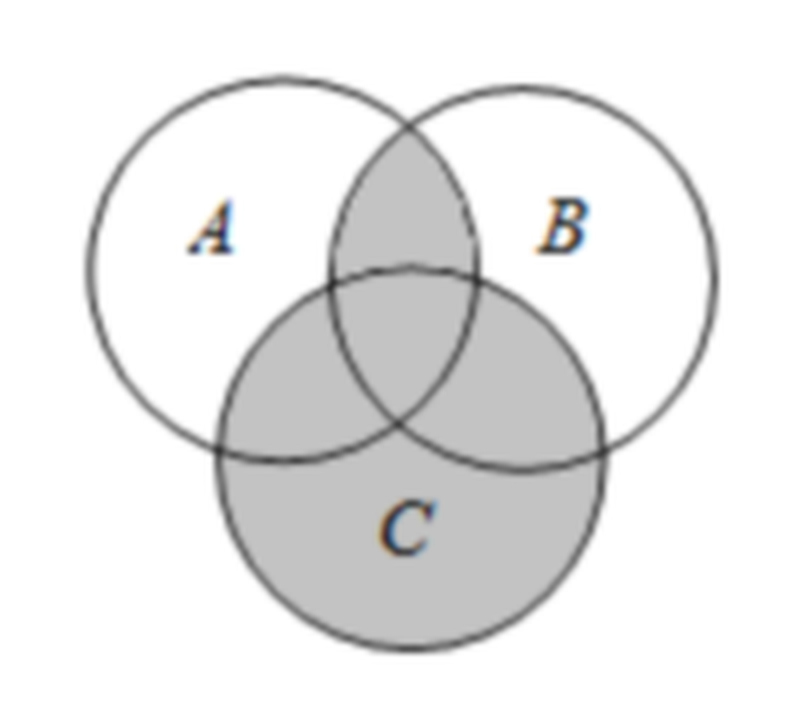
\includegraphics[width=0.30\textwidth]{figures/venn_ABcap_plus_C.png}
\end{center}

\keepwithprev
A. $(A\cup C)\cap(B\cup C)$\qquad B. $(A\cup B)\cap(A\cup C)$

C. $(A\cup B)\cap(B\cup C)$\qquad D. $(A\cup B)\cap C$

\ans{$A$}

\item 设 $f(x)=(x^2-6x+c_1)(x^2-6x+c_2)$，其中 $c_1\geqslant c_2$，集合

$M=\{x\mid f(x)=0\}=\{x_1,x_2,x_3\}\sub\Z$，则下列命题中不正确的是\mbox{（\quad）}

\keepwithprev
A. $3\in M$\qquad B. $c_2$ 可能为 $-16$

C. $c_1$ 可能为 $8$\qquad D. $M$ 中所有元素的和一定为 $9$

\ans{$C$}

\ifanswer
\solbegin
\step{若 $c_1$ 为 $8$，则 $c_2=9$，与 $c_1\geqslant c_2$ 矛盾，故选 $C$.}
\solend

\fi

\item 非空集合 $A$ 具有如下性质：①若 $x$、$y\in A$，则 $\dfrac{x}{y}\in A$；②若 $x$、$y\in A$，
则 $x+y\in A$；

由此可知：下列判断中，错误的是\mbox{（\quad）}

\keepwithprev
A. $-1\notin A$\qquad B. $\dfrac{2025}{2026}\in A$

C. 若 $x$、$y\in A$，则 $xy\in A$\qquad D. 若 $x$、$y\in A$，则 $x-y\in A$

\ans{$D$}

\ifanswer
\solbegin
\step{由题意得 $0\notin A$，$1\in A$，}
\step{对于 $A$，假设 $-1\in A$，则 $-1+1=0\in A$，矛盾，所以 $-1\notin A$，故 $A$ 正确；}
\step{对于 $B$，由 $1\in A$，得 $1+1=2\in A$，$2+1=3\in A$，$\cdots$，$2025\in A$，$2026\in A$，}
\step{所以 $\dfrac{2025}{2026}\in A$，故 $B$ 正确；}
\step{对于 $C$，因为 $1\in A$，$x\in A$，所以 $\dfrac1x\in A$，又因为 $y\in A$，
所以 $\dfrac{y}{\frac1x}=xy\in A$，}
\step{故 $C$ 正确；}
\step{对于 $D$，因为 $1\in A$，$2\in A$，若 $x=1$，$y=2$，则 $x-y=-1\notin A$，故 $D$ 错误.}
\step{故选 $D$.}
\solend

\fi

\end{enumerate}

\bigsec{三、解答题}

\begin{enumerate}
\setcounter{enumi}{13}

% 注：原卷本题题干把「$=0$」印在右花括号之外（$A=\{x\mid x^2-mx+4m-16\}=0$），
%     而其自己的【解析】印在括号之内（$A=\{x\mid x^2-mx+4m-16=0\}$）——原卷前后不一致，
%     本稿按解析与题目本意把 $=0$ 排在括号内，见文件头「排版差异」⑧。
\item 已知集合 $A=\{x\mid x^2-mx+4m-16=0\}$，$B=\{x\mid 1<x<4,x\in\N\}$，
$C=\{x\mid ax+2>0\}$，若 $A\cap B\neq\varnothing$，$A\cap C=\varnothing$，求实数 $m$ 的值以及
相应实数 $a$ 的取值范围.

\ifanswer
\solbegin
\step{集合 $A=\{x\mid x^2-mx+4m-16=0\}$，由 $\Delta=(-m)^2-4(4m-16)=(m-8)^2\geqslant0$，}
\step{所以当 $m=8$ 时，集合 $A=\{4\}$，当 $m\neq8$ 时，集合
$A=\left\{\dfrac{m-|m-8|}{2},\dfrac{m+|m-8|}{2}\right\}$，}
\step{集合 $B=\{x\mid 1<x<4,x\in\N\}$，得集合 $B=\{2,3\}$.}
\step{集合 $C=\{x\mid ax+2>0\}$，当 $a=0$ 时，集合 $C=\{x\mid x\in\R\}$，}
\step{当 $a<0$ 时，集合 $C=\left\{x\mid x<\dfrac2a\right\}$，当 $a>0$ 时，集合
$C=\left\{x\mid x>\dfrac2a\right\}$，}
\step{由 $A\cap B$ 非空得，$m=6$ 时，集合 $A=\{2,4\}$，$m=7$ 时，集合 $A=\{3,4\}$.}
\step{由 $A\cap C=\varnothing$，得 $m=6$ 或 $m=7$ 时，$a<0$ 或 $0<a<\dfrac12$ 符合要求.}
\solend

\fi

\ansspace[9]

\item 已知 $a>b>c$，$a+b+c=0$，方程 $ax^2+bx+c=0$ 的两个实根为 $x_1$、$x_2$.

\begin{enumerate}[label=(\arabic*)]
\item 证明：$-\dfrac12<\dfrac ba<1$；
% 注：此小问前加了 4pt 间距——不加时紧凑版该行的 $x_1^2$ 上标与下标恰好同箱，
%     pdftotext 抽正文会把上标当重影丢掉，make check 的正文指纹就对不上（纯抽取抖动，
%     版面与内容无差别，见 2026-09-20 入库注）。
\vspace{4pt}
\item 若 $x_1^2+x_1x_2+x_2^2=1$，求 $x_1^2-x_1x_2+x_2^2$.
\end{enumerate}

\ifanswer
\solbegin
\stepm{(1)}{因为 $a>b>c$，$a+b+c=0$，所以 $a>0$，$c<0$，$c=-a-b$，}
\step{由 $a>b$ 得 $\dfrac ba<1$ ①，由 $b>c$ 得 $b>-a-b$，即 $2b>-a$，即 $\dfrac ba>-\dfrac12$ ②，}
\step{由①②得 $-\dfrac12<\dfrac ba<1$；}
\stepm{(2)}{若 $x_1^2+x_1x_2+x_2^2=1$，则 $(x_1+x_2)^2-x_1x_2=1$，}
% 注：本行的连等式与原卷自己的结论对不上（照抄原卷、未改）——原卷印作
%     (b/a)²-b/a+1=1，则解出的应是 0 或 1；按 c=-a-b 应为 (b/a)²+b/a+1=1，
%     解得 0 或 -1（-1 因 c<0 舍去），恰与下一行「0 或 -1（舍去）」吻合。
%     详见文件头「原卷存疑」①。
\step{则 $\left(\dfrac ba\right)^2-\dfrac ca=\dfrac{b^2-ac}{a^2}
=\left(\dfrac ba\right)^2-\dfrac ba+1=1$，解得 $\dfrac ba=0$ 或 $-1$（舍去），}
\step{故 $\dfrac ba=0$，$\dfrac ca=-1$，}
\step{所以 $x_1^2-x_1x_2+x_2^2=(x_1+x_2)^2-3x_1x_2=\left(\dfrac ba\right)^2-3\times\dfrac ca=3$.}
\solend

\fi

\ansspace[6]

\item 已知方程 $x^2+px+q=0$ 与方程 $x^2+(p-3)x+2q+1=0$ 分别都有两个不相等的实根，若
他们的解集分别为 $A$、$B$，且 $A\cup B=\{1,2,5\}$，求 $p$、$q$、$A$、$B$.

\ifanswer
\solbegin
\step{两方程分别有两个不相等的实数根，而根的并集只有 $3$ 个元素，}
\step{则两方程有一公共根. 分类讨论：}
\stepm{（1）}{公共根为 $1$ 时，$x=1$ 分别代入两方程：}
\step{$\begin{cases}p+q+1=0\\ p-3+2q+1+1=0\end{cases}$，解得 $p=-3$，$q=2$，}
\step{两方程变为 $x^2-3x+2=0$，解得 $x=1$ 或 $x=2$，}
\step{$x^2-6x+5=0$ 解得 $x=1$ 或 $x=5$，满足题意.}
\stepm{（2）}{公共根为 $2$ 时，$x=2$ 分别代入两方程：}
\step{$\begin{cases}4+2p+q=0\\ 4+2p-6+2q+1=0\end{cases}$，解得 $p=-\dfrac92$，$q=5$，}
\step{第一个方程变为 $2x^2-9x+10=0$，解得 $x=2$ 或 $x=\dfrac52$，不满足题意，舍去.}
\stepm{（3）}{公共根为 $5$ 时，$x=5$ 分别代入两方程：}
\step{$\begin{cases}25+5p+q=0\\ 25+5p-15+2q+1=0\end{cases}$，解得 $p=-\dfrac{39}{5}$，$q=14$，}
\step{第一个方程变为 $5x^2-39x+70=0$，解得 $x=5$ 或 $x=\dfrac{14}{5}$，不满足题意，舍去.}
\step{综上，$p=-3$，$q=2$，$A=\{1,2\}$，$B=\{1,5\}$.}
\solend

\fi

\ansspace[8]

\item 对于集合 $A=\{a_1,a_2,\cdots,a_n\}(n\in\Z,n\geqslant3)$，其中每个元素均为正整数，如果
任意去掉其
中一个元素 $a_i(i=1,2,3\cdots,n)$ 之后，剩余的所有元素组成集合 $A_i(i=1,2,\cdots,n)$，并且
$A_i$ 都能分为两个集合 $B$ 和 $C$，满足 $B\cap C=\varnothing,B\cup C=A_i$，其中 $B$ 和 $C$
的所有元素之和相
等，就称集合 $A$ 为“可分集合”.

\begin{enumerate}[label=(\arabic*)]
\item 判断集合 $\{1,3,5,7,9,11,13\}$ 是否是“可分集合”（不必写过程）；
\item 用反证法证明：五个元素的集合 $A=\{a_1,a_2,a_3,a_4,a_5\}$ 一定不是“可分集合”；
\item 已知集合 $A=\{a_1,a_2,\cdots,a_n\}(n\in\Z,n\geqslant3)$ 是“可分集合”，求 $n$ 的最小值.
\end{enumerate}

\ifanswer
\solbegin
\stepm{(1)}{集合 $\{1,3,5,7,9,11,13\}$ 是“可分集合”；}
\stepm{(2)}{不妨设 $a_1<a_2<a_3<a_4<a_5$，}
\step{若去掉的元素为 $a_2$，将集合 $\{a_1,a_3,a_4,a_5\}$ 分成两个交集为空集的子集，}
\step{且两个子集元素之和相等，则有 $a_1+a_5=a_3+a_4$ ①，或者 $a_5=a_1+a_3+a_4$ ②；}
\step{若去掉的元素为 $a_1$，将集合 $\{a_2,a_3,a_4,a_5\}$ 分成两个交集为空集的子集，}
\step{且两个子集元素之和相等，则有 $a_2+a_5=a_3+a_4$ ③，或者 $a_5=a_2+a_3+a_4$ ④.}
\step{由①、③，得 $a_1=a_2$，矛盾；由①、④，得 $a_1=-a_2$，矛盾；}
\step{由②、③，得 $a_1=-a_2$，矛盾；由②、④，得 $a_1=a_2$ 矛盾.}
\step{因此当 $n=5$ 时，集合一定不是“可分集合”；}
\stepm{(3)}{①设集合 $A=\{a_1,a_2,\cdots,a_n\}$ 的所有元素之和为 $M$.}
\step{由题意得 $M-a_i(i=1,2,\cdots,n)$ 均为偶数，}
\step{因此 $a_i(i=1,2,\cdots,n)$ 均为奇数或偶数.}
\step{如果 $M$ 为奇数，则 $a_i(i=1,2,\cdots,n)$ 也均为奇数，}
\step{由于 $M=a_1+a_2+\cdots+a_n$，所以 $n$ 为奇数.}
\step{如果 $M$ 为偶数，则 $M-a_i(i=1,2,\cdots,n)$ 均为偶数，此时设 $a_i=2b_i$，}
\step{则 $\{b_1,b_2,\cdots,b_n\}$ 也是“可分集合”.}
\step{重复上述操作有限次，便可得各项均为奇数的“可分集合”，}
\step{此时各项之和也为奇数，则集合 $A$ 中元素个数 $n$ 为奇数.}
\step{综上所述，集合 $A$ 中元素个数为奇数.}
\step{②当 $n=3$ 时，显然任意集合 $\{a_1,a_2,a_3\}$ 不是“可分集合”.}
\step{当 $n=5$ 时，第（2）问已经证明不是“可分集合”.}
\step{当 $n=7$ 时，集合 $A=\{1,3,5,7,9,11,13\}$，}
\step{因为 $3+5+7+9=11+13$，$1+9+13=5+7+11$，$9+13=1+3+7+11$，}
\step{$1+3+5+11=7+13$，$1+9+11=3+5+13$，$3+7+9=1+5+13$，}
\step{$1+3+5+9=7+11$，则集合 $A$ 是“可分集合”，}
\step{所以集合 $A$ 中元素个数 $n$ 的最小值是 $7$.}
\solend

\fi

\ansspace*[10]

\end{enumerate}

\end{document}
"
% 紧凑版：xelatex "\def\iscompact{1}% 高一24_复旦附中_周末作业3.tex
%   —— 高一上数学「2026-2027 年复旦附中高一上周末作业 3」（试卷版/答案版）
% 试卷版：xelatex 高一24_复旦附中_周末作业3.tex
% 答案版：xelatex "\def\isanswer{1}% 高一24_复旦附中_周末作业3.tex
%   —— 高一上数学「2026-2027 年复旦附中高一上周末作业 3」（试卷版/答案版）
% 试卷版：xelatex 高一24_复旦附中_周末作业3.tex
% 答案版：xelatex "\def\isanswer{1}\input{高一24_复旦附中_周末作业3.tex}"
% 紧凑版：xelatex "\def\iscompact{1}\input{高一24_复旦附中_周末作业3.tex}"
%
% 原始材料是微信公众号图文（公众号「魔都数学加油站」连载「27学年高一 24」，2026-09-19 发布，
% 原文标题「27学年高一24——2026-2027年上海市复旦附中高一上周末作业3集合与逻辑、等式的性质」），
% 正文为 7 张 PNG 页（1080×1527，各页同尺寸）。原文本身就是一份**讲评版**——题目下方直接印出
% 【答案】或【解析】。试题文字、答案与解析均照原卷录入，未改内容。
% 卷面上的粉色斜水印「魔都数学加油站」属水印，未录入。
%
% 卷首标题：原卷印作「2026-2027 年复旦附中高一上周末作业 3」（公众号标题里有「上海市」三字，
% 卷面标题行没有，本稿照卷面），年份区间按全稿惯例排 en dash，前缀照原卷保留「年」。
%
% 与原卷的排版差异（均已在 README「说明」中交代）：
%   ① 原文自**第 3 题**起（第 1、2 题未在该文中发布），故本稿题号亦自 3 起；
%   ② 原卷本就印有「一、填空题」「二、选择题」「三、解答题」三节标题，本稿照原卷分节，
%      只把标题改排成全稿统一的「大节标题」样式；
%   ③ 原卷第 11 题的答案「A」直接印在题干末尾的括号内，第 12、13 题的括号空着、答案写在
%      解析末句「故选 C／D」里，本稿统一改为试卷版隐去、答案版以 \ans{} 给出（第 12、13 题
%      另附【解析】），使两版彻底分离；
%   ④ 原卷的集合／数集符号正体与粗体混用（第 8 题题干的 $\mathbf{R}$、第 9 题题干的
%      $\mathbf{N}$、第 12 题题干的 $\mathbf{Z}$ 为粗体，第 14 题解析的 $N$、$R$ 为斜体），
%      本稿按全稿惯例统一写作 $\R$、$\N$、$\Z$；
%   ⑤ 原卷填空的横线约两个字宽，本稿按全稿惯例统一排 \blankline[4.4em]；
%   ⑥ 第 11 题的 Venn 图原卷印在上一页末尾（第 10 题解析右侧、「二、选择题」标题旁），
%      本稿移至第 11 题题干之后；图取原卷截图、4× LANCZOS 放大
%      （figures/venn_ABcap_plus_C.png，阴影为 $A\cap B$ 的交与整个 $C$，即 $(A\cap B)\cup C$）；
%   ⑦ 原卷自印副标题「集合与逻辑、等式的性质」，本稿照录（与 高一14 同例，未改用惯例副标题）；
%   ⑧ 第 14 题题干原卷把「$=0$」印在右花括号**之外**（作
%      $A=\{x\mid x^2-mx+4m-16\}=0$），而它**自己的【解析】却印在括号之内**
%      （作 $A=\{x\mid x^2-mx+4m-16=0\}$）——原卷前后不一致；按原卷解析与题目本意，
%      本稿题干的 $=0$ 排在括号**之内**（与 高一b 第 13 题「原卷漏排 $A=$，本稿补上」同例）。
%
% 原卷存疑一处（已放大到能看清字形后核对，无法确证原意，本稿照抄原卷、未改）：
%   ① 第 15(2)【解析】的连等式印作
%      $\left(\frac ba\right)^2-\frac ca=\frac{b^2-ac}{a^2}=\left(\frac ba\right)^2-\frac ba+1=1$，
%      解得 $\frac ba=0$ 或 $-1$（舍去）——但由 $c=-a-b$ 应得 $\frac{b^2-ac}{a^2}
%      =\left(\frac ba\right)^2+\frac ba+1$（原卷把「$+\frac ba$」印成了「$-\frac ba$」）：
%      按原卷那行解出的是 $0$ 或 $1$，与其自己的结论「$0$ 或 $-1$」对不上；而按
%      $+\frac ba$ 解恰得 $0$ 或 $-1$（$-1$ 因 $c<0$ 舍去），与后文吻合。原卷显系笔误，
%      本稿照抄原卷（见源码中该处上方注释）。

\documentclass[a4paper,11pt]{article}
\usepackage{common}

\begin{document}

\examtitlest[3]{2026--2027 年复旦附中高一上周末作业 3}{集合与逻辑、等式的性质}

\bigsec{一、填空题}

\begin{enumerate}
\setcounter{enumi}{2}

\item 设 $M=\{x\mid y^2=x+2\}$，$N=\{x\mid y^2=-2x+8\}$，则 $M\cap N=$ \blankline[4.4em].

\ifanswer
\solbegin
\step{$M=[-2,+\infty)$，$N=(-\infty,4]$，则 $M\cap N=[-2,4]$.}
\solend

\fi

\item 若“$x\geqslant a$”是“$|x|\leqslant2$”的必要条件，则实数 $a$ 的取值集合是 \blankline[4.4em].

\ans{$(-\infty,-2]$}

\item 某校一年级的 $200$ 人中，爱好数学的有 $95$ 人，爱好体育的有 $156$ 人，则数学体育都爱好
的至少有 \blankline[4.4em] 人.

\ifanswer
\solbegin
\step{数学体育都爱好的至少有 $95+156-200=51$ 人.}
\solend

\fi

\item 已知 $x$ 为实数，且 $x^2+\dfrac{1}{x^2}=3$，则 $x^3+\dfrac{1}{x^3}$ 的值是 \blankline[4.4em].

\ifanswer
\solbegin
\step{因为 $x^2+\dfrac{1}{x^2}=\left(x+\dfrac1x\right)^2-2=3$，所以 $x+\dfrac1x=\pm\sqrt5$，}
\step{所以 $x^3+\dfrac{1}{x^3}=\left(x+\dfrac1x\right)\left(x^2-1+\dfrac{1}{x^2}\right)=\pm2\sqrt5$.}
\solend

\fi

\item 非空集合 $A=\{x\mid a+1\leqslant x<2a-1\}$，$B=\{x\mid-2\leqslant x\leqslant5\}$，
若 $A\sub(A\cap B)$，则 $a$ 的取值范围是 \blankline[4.4em].

\ifanswer
\solbegin
\step{当 $a+1<2a-1$，即 $a>2$ 时，$A\neq\varnothing$，由 $A\sub(A\cap B)$ 得 $A\sub B$，}
\step{得 $\begin{cases}a+1\geqslant-2\\ 2a-1\leqslant5\end{cases}$，解得 $-3\leqslant a\leqslant3$，所以 $2<a\leqslant3$.}
\solend

\fi

\item 已知集合 $\{x\mid(x-1)(x^2-x+a)=0,x\in\R\}$ 中的所有元素之和为 $1$，则实数 $a$ 的取值范
围是 \blankline[4.4em].

\ifanswer
\solbegin
\step{令 $x-1=0$，得 $x=1$，}
\stepm{①}{若 $x^2-x+a=0$ 无实数根，则 $\Delta=1-4a<0$，解得 $a>\dfrac14$，}
\step{此时集合只有元素 $1$，符合题意；}
\stepm{②}{若 $x^2-x+a=0$ 有两个相等的实数根，则 $\Delta=1-4a=0$，解得 $a=\dfrac14$，}
\step{此时方程为 $x^2-x+\dfrac14=0$，解得 $x=\dfrac12$，此时集合为 $\left\{1,\dfrac12\right\}$，不合题意；}
\stepm{③}{若 $x^2-x+a=0$ 有两个不相等的实数根，则 $\Delta=1-4a>0$，解得 $a<\dfrac14$，}
\step{设方程 $x^2-x+a=0$ 的两个实根分别为 $x_1,x_2$，则 $x_1+x_2=1$，}
\step{若 $x_1\neq1,x_2\neq1$，则集合为 $\{1,x_1,x_2\}$，不合题意，}
\step{若 $x_1=1$，则 $x_2=0$，此时集合为 $\{1,0\}$，符合题意，所以 $a=x_1x_2=0$，}
\step{综上所述，实数 $a$ 的取值范围是 $\{0\}\cup\left(\dfrac14,+\infty\right)$.}
\solend

\fi

\item 集合 $A=\{m\mid m=2k,k\in\N,1\leqslant k\leqslant50\}$，
$B=\{n\mid n=i+j,i<j,i\in A,j\in A\}$，则 $B$ 中元素的个数是 \blankline[4.4em].

\ifanswer
\solbegin
\step{$B$ 中最小元素是 $6$，最大元素是 $198$，则 $B$ 中元素的个数是 $\dfrac{198-6}{2}+1=97$.}
\solend

\fi

\item 关于 $(x,y,z)$ 的方程组
$\begin{cases}x^2+y^2+25z^2=6zx+8yz\\ 3x^2+2y^2+z^2=240\end{cases}$ 的解集为 \blankline[4.4em].

\ifanswer
\solbegin
\step{由上式得 $(x^2-6xz+9z^2)+(y^2-8yz+16z^2)=0$，}
\step{则 $(x-3z)^2+(y-4z)^2=0$，}
\step{所以 $(x,y,z)=(3t,4t,t)$，$t$ 为实数，代入下式中 $27\cdot t^2+32t^2+t^2=60t^2=240$，}
\step{则 $t^2=4$，$t=\pm2$，所以 $(x,y,z)=(6,8,2),(-6,-8,-2)$.}
\solend

\fi

\end{enumerate}

\bigsec{二、选择题}

\begin{enumerate}
\setcounter{enumi}{10}

\item 下列表示图形中的阴影部分的是\mbox{（\quad）}

\begin{center}
% 图取原卷截图、4× LANCZOS 放大（原卷把图印在上一页末尾，本稿移至此处，见文件头⑥）。
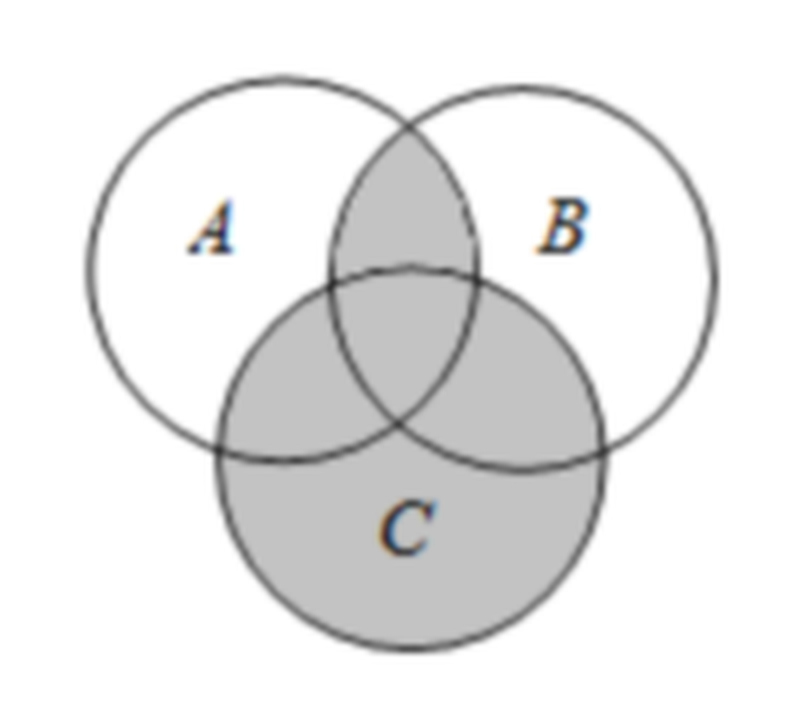
\includegraphics[width=0.30\textwidth]{figures/venn_ABcap_plus_C.png}
\end{center}

\keepwithprev
A. $(A\cup C)\cap(B\cup C)$\qquad B. $(A\cup B)\cap(A\cup C)$

C. $(A\cup B)\cap(B\cup C)$\qquad D. $(A\cup B)\cap C$

\ans{$A$}

\item 设 $f(x)=(x^2-6x+c_1)(x^2-6x+c_2)$，其中 $c_1\geqslant c_2$，集合

$M=\{x\mid f(x)=0\}=\{x_1,x_2,x_3\}\sub\Z$，则下列命题中不正确的是\mbox{（\quad）}

\keepwithprev
A. $3\in M$\qquad B. $c_2$ 可能为 $-16$

C. $c_1$ 可能为 $8$\qquad D. $M$ 中所有元素的和一定为 $9$

\ans{$C$}

\ifanswer
\solbegin
\step{若 $c_1$ 为 $8$，则 $c_2=9$，与 $c_1\geqslant c_2$ 矛盾，故选 $C$.}
\solend

\fi

\item 非空集合 $A$ 具有如下性质：①若 $x$、$y\in A$，则 $\dfrac{x}{y}\in A$；②若 $x$、$y\in A$，
则 $x+y\in A$；

由此可知：下列判断中，错误的是\mbox{（\quad）}

\keepwithprev
A. $-1\notin A$\qquad B. $\dfrac{2025}{2026}\in A$

C. 若 $x$、$y\in A$，则 $xy\in A$\qquad D. 若 $x$、$y\in A$，则 $x-y\in A$

\ans{$D$}

\ifanswer
\solbegin
\step{由题意得 $0\notin A$，$1\in A$，}
\step{对于 $A$，假设 $-1\in A$，则 $-1+1=0\in A$，矛盾，所以 $-1\notin A$，故 $A$ 正确；}
\step{对于 $B$，由 $1\in A$，得 $1+1=2\in A$，$2+1=3\in A$，$\cdots$，$2025\in A$，$2026\in A$，}
\step{所以 $\dfrac{2025}{2026}\in A$，故 $B$ 正确；}
\step{对于 $C$，因为 $1\in A$，$x\in A$，所以 $\dfrac1x\in A$，又因为 $y\in A$，
所以 $\dfrac{y}{\frac1x}=xy\in A$，}
\step{故 $C$ 正确；}
\step{对于 $D$，因为 $1\in A$，$2\in A$，若 $x=1$，$y=2$，则 $x-y=-1\notin A$，故 $D$ 错误.}
\step{故选 $D$.}
\solend

\fi

\end{enumerate}

\bigsec{三、解答题}

\begin{enumerate}
\setcounter{enumi}{13}

% 注：原卷本题题干把「$=0$」印在右花括号之外（$A=\{x\mid x^2-mx+4m-16\}=0$），
%     而其自己的【解析】印在括号之内（$A=\{x\mid x^2-mx+4m-16=0\}$）——原卷前后不一致，
%     本稿按解析与题目本意把 $=0$ 排在括号内，见文件头「排版差异」⑧。
\item 已知集合 $A=\{x\mid x^2-mx+4m-16=0\}$，$B=\{x\mid 1<x<4,x\in\N\}$，
$C=\{x\mid ax+2>0\}$，若 $A\cap B\neq\varnothing$，$A\cap C=\varnothing$，求实数 $m$ 的值以及
相应实数 $a$ 的取值范围.

\ifanswer
\solbegin
\step{集合 $A=\{x\mid x^2-mx+4m-16=0\}$，由 $\Delta=(-m)^2-4(4m-16)=(m-8)^2\geqslant0$，}
\step{所以当 $m=8$ 时，集合 $A=\{4\}$，当 $m\neq8$ 时，集合
$A=\left\{\dfrac{m-|m-8|}{2},\dfrac{m+|m-8|}{2}\right\}$，}
\step{集合 $B=\{x\mid 1<x<4,x\in\N\}$，得集合 $B=\{2,3\}$.}
\step{集合 $C=\{x\mid ax+2>0\}$，当 $a=0$ 时，集合 $C=\{x\mid x\in\R\}$，}
\step{当 $a<0$ 时，集合 $C=\left\{x\mid x<\dfrac2a\right\}$，当 $a>0$ 时，集合
$C=\left\{x\mid x>\dfrac2a\right\}$，}
\step{由 $A\cap B$ 非空得，$m=6$ 时，集合 $A=\{2,4\}$，$m=7$ 时，集合 $A=\{3,4\}$.}
\step{由 $A\cap C=\varnothing$，得 $m=6$ 或 $m=7$ 时，$a<0$ 或 $0<a<\dfrac12$ 符合要求.}
\solend

\fi

\ansspace[9]

\item 已知 $a>b>c$，$a+b+c=0$，方程 $ax^2+bx+c=0$ 的两个实根为 $x_1$、$x_2$.

\begin{enumerate}[label=(\arabic*)]
\item 证明：$-\dfrac12<\dfrac ba<1$；
% 注：此小问前加了 4pt 间距——不加时紧凑版该行的 $x_1^2$ 上标与下标恰好同箱，
%     pdftotext 抽正文会把上标当重影丢掉，make check 的正文指纹就对不上（纯抽取抖动，
%     版面与内容无差别，见 2026-09-20 入库注）。
\vspace{4pt}
\item 若 $x_1^2+x_1x_2+x_2^2=1$，求 $x_1^2-x_1x_2+x_2^2$.
\end{enumerate}

\ifanswer
\solbegin
\stepm{(1)}{因为 $a>b>c$，$a+b+c=0$，所以 $a>0$，$c<0$，$c=-a-b$，}
\step{由 $a>b$ 得 $\dfrac ba<1$ ①，由 $b>c$ 得 $b>-a-b$，即 $2b>-a$，即 $\dfrac ba>-\dfrac12$ ②，}
\step{由①②得 $-\dfrac12<\dfrac ba<1$；}
\stepm{(2)}{若 $x_1^2+x_1x_2+x_2^2=1$，则 $(x_1+x_2)^2-x_1x_2=1$，}
% 注：本行的连等式与原卷自己的结论对不上（照抄原卷、未改）——原卷印作
%     (b/a)²-b/a+1=1，则解出的应是 0 或 1；按 c=-a-b 应为 (b/a)²+b/a+1=1，
%     解得 0 或 -1（-1 因 c<0 舍去），恰与下一行「0 或 -1（舍去）」吻合。
%     详见文件头「原卷存疑」①。
\step{则 $\left(\dfrac ba\right)^2-\dfrac ca=\dfrac{b^2-ac}{a^2}
=\left(\dfrac ba\right)^2-\dfrac ba+1=1$，解得 $\dfrac ba=0$ 或 $-1$（舍去），}
\step{故 $\dfrac ba=0$，$\dfrac ca=-1$，}
\step{所以 $x_1^2-x_1x_2+x_2^2=(x_1+x_2)^2-3x_1x_2=\left(\dfrac ba\right)^2-3\times\dfrac ca=3$.}
\solend

\fi

\ansspace[6]

\item 已知方程 $x^2+px+q=0$ 与方程 $x^2+(p-3)x+2q+1=0$ 分别都有两个不相等的实根，若
他们的解集分别为 $A$、$B$，且 $A\cup B=\{1,2,5\}$，求 $p$、$q$、$A$、$B$.

\ifanswer
\solbegin
\step{两方程分别有两个不相等的实数根，而根的并集只有 $3$ 个元素，}
\step{则两方程有一公共根. 分类讨论：}
\stepm{（1）}{公共根为 $1$ 时，$x=1$ 分别代入两方程：}
\step{$\begin{cases}p+q+1=0\\ p-3+2q+1+1=0\end{cases}$，解得 $p=-3$，$q=2$，}
\step{两方程变为 $x^2-3x+2=0$，解得 $x=1$ 或 $x=2$，}
\step{$x^2-6x+5=0$ 解得 $x=1$ 或 $x=5$，满足题意.}
\stepm{（2）}{公共根为 $2$ 时，$x=2$ 分别代入两方程：}
\step{$\begin{cases}4+2p+q=0\\ 4+2p-6+2q+1=0\end{cases}$，解得 $p=-\dfrac92$，$q=5$，}
\step{第一个方程变为 $2x^2-9x+10=0$，解得 $x=2$ 或 $x=\dfrac52$，不满足题意，舍去.}
\stepm{（3）}{公共根为 $5$ 时，$x=5$ 分别代入两方程：}
\step{$\begin{cases}25+5p+q=0\\ 25+5p-15+2q+1=0\end{cases}$，解得 $p=-\dfrac{39}{5}$，$q=14$，}
\step{第一个方程变为 $5x^2-39x+70=0$，解得 $x=5$ 或 $x=\dfrac{14}{5}$，不满足题意，舍去.}
\step{综上，$p=-3$，$q=2$，$A=\{1,2\}$，$B=\{1,5\}$.}
\solend

\fi

\ansspace[8]

\item 对于集合 $A=\{a_1,a_2,\cdots,a_n\}(n\in\Z,n\geqslant3)$，其中每个元素均为正整数，如果
任意去掉其
中一个元素 $a_i(i=1,2,3\cdots,n)$ 之后，剩余的所有元素组成集合 $A_i(i=1,2,\cdots,n)$，并且
$A_i$ 都能分为两个集合 $B$ 和 $C$，满足 $B\cap C=\varnothing,B\cup C=A_i$，其中 $B$ 和 $C$
的所有元素之和相
等，就称集合 $A$ 为“可分集合”.

\begin{enumerate}[label=(\arabic*)]
\item 判断集合 $\{1,3,5,7,9,11,13\}$ 是否是“可分集合”（不必写过程）；
\item 用反证法证明：五个元素的集合 $A=\{a_1,a_2,a_3,a_4,a_5\}$ 一定不是“可分集合”；
\item 已知集合 $A=\{a_1,a_2,\cdots,a_n\}(n\in\Z,n\geqslant3)$ 是“可分集合”，求 $n$ 的最小值.
\end{enumerate}

\ifanswer
\solbegin
\stepm{(1)}{集合 $\{1,3,5,7,9,11,13\}$ 是“可分集合”；}
\stepm{(2)}{不妨设 $a_1<a_2<a_3<a_4<a_5$，}
\step{若去掉的元素为 $a_2$，将集合 $\{a_1,a_3,a_4,a_5\}$ 分成两个交集为空集的子集，}
\step{且两个子集元素之和相等，则有 $a_1+a_5=a_3+a_4$ ①，或者 $a_5=a_1+a_3+a_4$ ②；}
\step{若去掉的元素为 $a_1$，将集合 $\{a_2,a_3,a_4,a_5\}$ 分成两个交集为空集的子集，}
\step{且两个子集元素之和相等，则有 $a_2+a_5=a_3+a_4$ ③，或者 $a_5=a_2+a_3+a_4$ ④.}
\step{由①、③，得 $a_1=a_2$，矛盾；由①、④，得 $a_1=-a_2$，矛盾；}
\step{由②、③，得 $a_1=-a_2$，矛盾；由②、④，得 $a_1=a_2$ 矛盾.}
\step{因此当 $n=5$ 时，集合一定不是“可分集合”；}
\stepm{(3)}{①设集合 $A=\{a_1,a_2,\cdots,a_n\}$ 的所有元素之和为 $M$.}
\step{由题意得 $M-a_i(i=1,2,\cdots,n)$ 均为偶数，}
\step{因此 $a_i(i=1,2,\cdots,n)$ 均为奇数或偶数.}
\step{如果 $M$ 为奇数，则 $a_i(i=1,2,\cdots,n)$ 也均为奇数，}
\step{由于 $M=a_1+a_2+\cdots+a_n$，所以 $n$ 为奇数.}
\step{如果 $M$ 为偶数，则 $M-a_i(i=1,2,\cdots,n)$ 均为偶数，此时设 $a_i=2b_i$，}
\step{则 $\{b_1,b_2,\cdots,b_n\}$ 也是“可分集合”.}
\step{重复上述操作有限次，便可得各项均为奇数的“可分集合”，}
\step{此时各项之和也为奇数，则集合 $A$ 中元素个数 $n$ 为奇数.}
\step{综上所述，集合 $A$ 中元素个数为奇数.}
\step{②当 $n=3$ 时，显然任意集合 $\{a_1,a_2,a_3\}$ 不是“可分集合”.}
\step{当 $n=5$ 时，第（2）问已经证明不是“可分集合”.}
\step{当 $n=7$ 时，集合 $A=\{1,3,5,7,9,11,13\}$，}
\step{因为 $3+5+7+9=11+13$，$1+9+13=5+7+11$，$9+13=1+3+7+11$，}
\step{$1+3+5+11=7+13$，$1+9+11=3+5+13$，$3+7+9=1+5+13$，}
\step{$1+3+5+9=7+11$，则集合 $A$ 是“可分集合”，}
\step{所以集合 $A$ 中元素个数 $n$ 的最小值是 $7$.}
\solend

\fi

\ansspace*[10]

\end{enumerate}

\end{document}
"
% 紧凑版：xelatex "\def\iscompact{1}% 高一24_复旦附中_周末作业3.tex
%   —— 高一上数学「2026-2027 年复旦附中高一上周末作业 3」（试卷版/答案版）
% 试卷版：xelatex 高一24_复旦附中_周末作业3.tex
% 答案版：xelatex "\def\isanswer{1}\input{高一24_复旦附中_周末作业3.tex}"
% 紧凑版：xelatex "\def\iscompact{1}\input{高一24_复旦附中_周末作业3.tex}"
%
% 原始材料是微信公众号图文（公众号「魔都数学加油站」连载「27学年高一 24」，2026-09-19 发布，
% 原文标题「27学年高一24——2026-2027年上海市复旦附中高一上周末作业3集合与逻辑、等式的性质」），
% 正文为 7 张 PNG 页（1080×1527，各页同尺寸）。原文本身就是一份**讲评版**——题目下方直接印出
% 【答案】或【解析】。试题文字、答案与解析均照原卷录入，未改内容。
% 卷面上的粉色斜水印「魔都数学加油站」属水印，未录入。
%
% 卷首标题：原卷印作「2026-2027 年复旦附中高一上周末作业 3」（公众号标题里有「上海市」三字，
% 卷面标题行没有，本稿照卷面），年份区间按全稿惯例排 en dash，前缀照原卷保留「年」。
%
% 与原卷的排版差异（均已在 README「说明」中交代）：
%   ① 原文自**第 3 题**起（第 1、2 题未在该文中发布），故本稿题号亦自 3 起；
%   ② 原卷本就印有「一、填空题」「二、选择题」「三、解答题」三节标题，本稿照原卷分节，
%      只把标题改排成全稿统一的「大节标题」样式；
%   ③ 原卷第 11 题的答案「A」直接印在题干末尾的括号内，第 12、13 题的括号空着、答案写在
%      解析末句「故选 C／D」里，本稿统一改为试卷版隐去、答案版以 \ans{} 给出（第 12、13 题
%      另附【解析】），使两版彻底分离；
%   ④ 原卷的集合／数集符号正体与粗体混用（第 8 题题干的 $\mathbf{R}$、第 9 题题干的
%      $\mathbf{N}$、第 12 题题干的 $\mathbf{Z}$ 为粗体，第 14 题解析的 $N$、$R$ 为斜体），
%      本稿按全稿惯例统一写作 $\R$、$\N$、$\Z$；
%   ⑤ 原卷填空的横线约两个字宽，本稿按全稿惯例统一排 \blankline[4.4em]；
%   ⑥ 第 11 题的 Venn 图原卷印在上一页末尾（第 10 题解析右侧、「二、选择题」标题旁），
%      本稿移至第 11 题题干之后；图取原卷截图、4× LANCZOS 放大
%      （figures/venn_ABcap_plus_C.png，阴影为 $A\cap B$ 的交与整个 $C$，即 $(A\cap B)\cup C$）；
%   ⑦ 原卷自印副标题「集合与逻辑、等式的性质」，本稿照录（与 高一14 同例，未改用惯例副标题）；
%   ⑧ 第 14 题题干原卷把「$=0$」印在右花括号**之外**（作
%      $A=\{x\mid x^2-mx+4m-16\}=0$），而它**自己的【解析】却印在括号之内**
%      （作 $A=\{x\mid x^2-mx+4m-16=0\}$）——原卷前后不一致；按原卷解析与题目本意，
%      本稿题干的 $=0$ 排在括号**之内**（与 高一b 第 13 题「原卷漏排 $A=$，本稿补上」同例）。
%
% 原卷存疑一处（已放大到能看清字形后核对，无法确证原意，本稿照抄原卷、未改）：
%   ① 第 15(2)【解析】的连等式印作
%      $\left(\frac ba\right)^2-\frac ca=\frac{b^2-ac}{a^2}=\left(\frac ba\right)^2-\frac ba+1=1$，
%      解得 $\frac ba=0$ 或 $-1$（舍去）——但由 $c=-a-b$ 应得 $\frac{b^2-ac}{a^2}
%      =\left(\frac ba\right)^2+\frac ba+1$（原卷把「$+\frac ba$」印成了「$-\frac ba$」）：
%      按原卷那行解出的是 $0$ 或 $1$，与其自己的结论「$0$ 或 $-1$」对不上；而按
%      $+\frac ba$ 解恰得 $0$ 或 $-1$（$-1$ 因 $c<0$ 舍去），与后文吻合。原卷显系笔误，
%      本稿照抄原卷（见源码中该处上方注释）。

\documentclass[a4paper,11pt]{article}
\usepackage{common}

\begin{document}

\examtitlest[3]{2026--2027 年复旦附中高一上周末作业 3}{集合与逻辑、等式的性质}

\bigsec{一、填空题}

\begin{enumerate}
\setcounter{enumi}{2}

\item 设 $M=\{x\mid y^2=x+2\}$，$N=\{x\mid y^2=-2x+8\}$，则 $M\cap N=$ \blankline[4.4em].

\ifanswer
\solbegin
\step{$M=[-2,+\infty)$，$N=(-\infty,4]$，则 $M\cap N=[-2,4]$.}
\solend

\fi

\item 若“$x\geqslant a$”是“$|x|\leqslant2$”的必要条件，则实数 $a$ 的取值集合是 \blankline[4.4em].

\ans{$(-\infty,-2]$}

\item 某校一年级的 $200$ 人中，爱好数学的有 $95$ 人，爱好体育的有 $156$ 人，则数学体育都爱好
的至少有 \blankline[4.4em] 人.

\ifanswer
\solbegin
\step{数学体育都爱好的至少有 $95+156-200=51$ 人.}
\solend

\fi

\item 已知 $x$ 为实数，且 $x^2+\dfrac{1}{x^2}=3$，则 $x^3+\dfrac{1}{x^3}$ 的值是 \blankline[4.4em].

\ifanswer
\solbegin
\step{因为 $x^2+\dfrac{1}{x^2}=\left(x+\dfrac1x\right)^2-2=3$，所以 $x+\dfrac1x=\pm\sqrt5$，}
\step{所以 $x^3+\dfrac{1}{x^3}=\left(x+\dfrac1x\right)\left(x^2-1+\dfrac{1}{x^2}\right)=\pm2\sqrt5$.}
\solend

\fi

\item 非空集合 $A=\{x\mid a+1\leqslant x<2a-1\}$，$B=\{x\mid-2\leqslant x\leqslant5\}$，
若 $A\sub(A\cap B)$，则 $a$ 的取值范围是 \blankline[4.4em].

\ifanswer
\solbegin
\step{当 $a+1<2a-1$，即 $a>2$ 时，$A\neq\varnothing$，由 $A\sub(A\cap B)$ 得 $A\sub B$，}
\step{得 $\begin{cases}a+1\geqslant-2\\ 2a-1\leqslant5\end{cases}$，解得 $-3\leqslant a\leqslant3$，所以 $2<a\leqslant3$.}
\solend

\fi

\item 已知集合 $\{x\mid(x-1)(x^2-x+a)=0,x\in\R\}$ 中的所有元素之和为 $1$，则实数 $a$ 的取值范
围是 \blankline[4.4em].

\ifanswer
\solbegin
\step{令 $x-1=0$，得 $x=1$，}
\stepm{①}{若 $x^2-x+a=0$ 无实数根，则 $\Delta=1-4a<0$，解得 $a>\dfrac14$，}
\step{此时集合只有元素 $1$，符合题意；}
\stepm{②}{若 $x^2-x+a=0$ 有两个相等的实数根，则 $\Delta=1-4a=0$，解得 $a=\dfrac14$，}
\step{此时方程为 $x^2-x+\dfrac14=0$，解得 $x=\dfrac12$，此时集合为 $\left\{1,\dfrac12\right\}$，不合题意；}
\stepm{③}{若 $x^2-x+a=0$ 有两个不相等的实数根，则 $\Delta=1-4a>0$，解得 $a<\dfrac14$，}
\step{设方程 $x^2-x+a=0$ 的两个实根分别为 $x_1,x_2$，则 $x_1+x_2=1$，}
\step{若 $x_1\neq1,x_2\neq1$，则集合为 $\{1,x_1,x_2\}$，不合题意，}
\step{若 $x_1=1$，则 $x_2=0$，此时集合为 $\{1,0\}$，符合题意，所以 $a=x_1x_2=0$，}
\step{综上所述，实数 $a$ 的取值范围是 $\{0\}\cup\left(\dfrac14,+\infty\right)$.}
\solend

\fi

\item 集合 $A=\{m\mid m=2k,k\in\N,1\leqslant k\leqslant50\}$，
$B=\{n\mid n=i+j,i<j,i\in A,j\in A\}$，则 $B$ 中元素的个数是 \blankline[4.4em].

\ifanswer
\solbegin
\step{$B$ 中最小元素是 $6$，最大元素是 $198$，则 $B$ 中元素的个数是 $\dfrac{198-6}{2}+1=97$.}
\solend

\fi

\item 关于 $(x,y,z)$ 的方程组
$\begin{cases}x^2+y^2+25z^2=6zx+8yz\\ 3x^2+2y^2+z^2=240\end{cases}$ 的解集为 \blankline[4.4em].

\ifanswer
\solbegin
\step{由上式得 $(x^2-6xz+9z^2)+(y^2-8yz+16z^2)=0$，}
\step{则 $(x-3z)^2+(y-4z)^2=0$，}
\step{所以 $(x,y,z)=(3t,4t,t)$，$t$ 为实数，代入下式中 $27\cdot t^2+32t^2+t^2=60t^2=240$，}
\step{则 $t^2=4$，$t=\pm2$，所以 $(x,y,z)=(6,8,2),(-6,-8,-2)$.}
\solend

\fi

\end{enumerate}

\bigsec{二、选择题}

\begin{enumerate}
\setcounter{enumi}{10}

\item 下列表示图形中的阴影部分的是\mbox{（\quad）}

\begin{center}
% 图取原卷截图、4× LANCZOS 放大（原卷把图印在上一页末尾，本稿移至此处，见文件头⑥）。
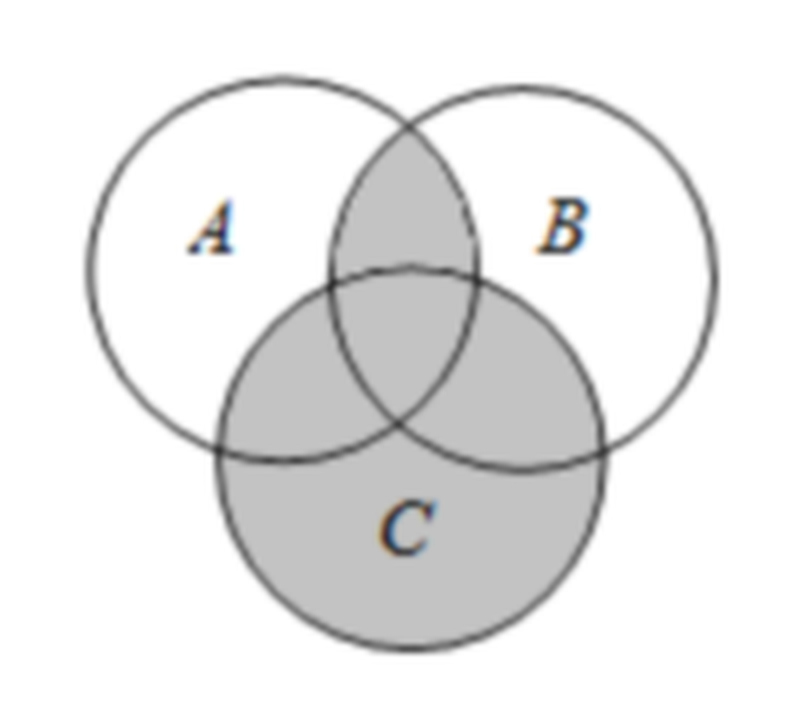
\includegraphics[width=0.30\textwidth]{figures/venn_ABcap_plus_C.png}
\end{center}

\keepwithprev
A. $(A\cup C)\cap(B\cup C)$\qquad B. $(A\cup B)\cap(A\cup C)$

C. $(A\cup B)\cap(B\cup C)$\qquad D. $(A\cup B)\cap C$

\ans{$A$}

\item 设 $f(x)=(x^2-6x+c_1)(x^2-6x+c_2)$，其中 $c_1\geqslant c_2$，集合

$M=\{x\mid f(x)=0\}=\{x_1,x_2,x_3\}\sub\Z$，则下列命题中不正确的是\mbox{（\quad）}

\keepwithprev
A. $3\in M$\qquad B. $c_2$ 可能为 $-16$

C. $c_1$ 可能为 $8$\qquad D. $M$ 中所有元素的和一定为 $9$

\ans{$C$}

\ifanswer
\solbegin
\step{若 $c_1$ 为 $8$，则 $c_2=9$，与 $c_1\geqslant c_2$ 矛盾，故选 $C$.}
\solend

\fi

\item 非空集合 $A$ 具有如下性质：①若 $x$、$y\in A$，则 $\dfrac{x}{y}\in A$；②若 $x$、$y\in A$，
则 $x+y\in A$；

由此可知：下列判断中，错误的是\mbox{（\quad）}

\keepwithprev
A. $-1\notin A$\qquad B. $\dfrac{2025}{2026}\in A$

C. 若 $x$、$y\in A$，则 $xy\in A$\qquad D. 若 $x$、$y\in A$，则 $x-y\in A$

\ans{$D$}

\ifanswer
\solbegin
\step{由题意得 $0\notin A$，$1\in A$，}
\step{对于 $A$，假设 $-1\in A$，则 $-1+1=0\in A$，矛盾，所以 $-1\notin A$，故 $A$ 正确；}
\step{对于 $B$，由 $1\in A$，得 $1+1=2\in A$，$2+1=3\in A$，$\cdots$，$2025\in A$，$2026\in A$，}
\step{所以 $\dfrac{2025}{2026}\in A$，故 $B$ 正确；}
\step{对于 $C$，因为 $1\in A$，$x\in A$，所以 $\dfrac1x\in A$，又因为 $y\in A$，
所以 $\dfrac{y}{\frac1x}=xy\in A$，}
\step{故 $C$ 正确；}
\step{对于 $D$，因为 $1\in A$，$2\in A$，若 $x=1$，$y=2$，则 $x-y=-1\notin A$，故 $D$ 错误.}
\step{故选 $D$.}
\solend

\fi

\end{enumerate}

\bigsec{三、解答题}

\begin{enumerate}
\setcounter{enumi}{13}

% 注：原卷本题题干把「$=0$」印在右花括号之外（$A=\{x\mid x^2-mx+4m-16\}=0$），
%     而其自己的【解析】印在括号之内（$A=\{x\mid x^2-mx+4m-16=0\}$）——原卷前后不一致，
%     本稿按解析与题目本意把 $=0$ 排在括号内，见文件头「排版差异」⑧。
\item 已知集合 $A=\{x\mid x^2-mx+4m-16=0\}$，$B=\{x\mid 1<x<4,x\in\N\}$，
$C=\{x\mid ax+2>0\}$，若 $A\cap B\neq\varnothing$，$A\cap C=\varnothing$，求实数 $m$ 的值以及
相应实数 $a$ 的取值范围.

\ifanswer
\solbegin
\step{集合 $A=\{x\mid x^2-mx+4m-16=0\}$，由 $\Delta=(-m)^2-4(4m-16)=(m-8)^2\geqslant0$，}
\step{所以当 $m=8$ 时，集合 $A=\{4\}$，当 $m\neq8$ 时，集合
$A=\left\{\dfrac{m-|m-8|}{2},\dfrac{m+|m-8|}{2}\right\}$，}
\step{集合 $B=\{x\mid 1<x<4,x\in\N\}$，得集合 $B=\{2,3\}$.}
\step{集合 $C=\{x\mid ax+2>0\}$，当 $a=0$ 时，集合 $C=\{x\mid x\in\R\}$，}
\step{当 $a<0$ 时，集合 $C=\left\{x\mid x<\dfrac2a\right\}$，当 $a>0$ 时，集合
$C=\left\{x\mid x>\dfrac2a\right\}$，}
\step{由 $A\cap B$ 非空得，$m=6$ 时，集合 $A=\{2,4\}$，$m=7$ 时，集合 $A=\{3,4\}$.}
\step{由 $A\cap C=\varnothing$，得 $m=6$ 或 $m=7$ 时，$a<0$ 或 $0<a<\dfrac12$ 符合要求.}
\solend

\fi

\ansspace[9]

\item 已知 $a>b>c$，$a+b+c=0$，方程 $ax^2+bx+c=0$ 的两个实根为 $x_1$、$x_2$.

\begin{enumerate}[label=(\arabic*)]
\item 证明：$-\dfrac12<\dfrac ba<1$；
% 注：此小问前加了 4pt 间距——不加时紧凑版该行的 $x_1^2$ 上标与下标恰好同箱，
%     pdftotext 抽正文会把上标当重影丢掉，make check 的正文指纹就对不上（纯抽取抖动，
%     版面与内容无差别，见 2026-09-20 入库注）。
\vspace{4pt}
\item 若 $x_1^2+x_1x_2+x_2^2=1$，求 $x_1^2-x_1x_2+x_2^2$.
\end{enumerate}

\ifanswer
\solbegin
\stepm{(1)}{因为 $a>b>c$，$a+b+c=0$，所以 $a>0$，$c<0$，$c=-a-b$，}
\step{由 $a>b$ 得 $\dfrac ba<1$ ①，由 $b>c$ 得 $b>-a-b$，即 $2b>-a$，即 $\dfrac ba>-\dfrac12$ ②，}
\step{由①②得 $-\dfrac12<\dfrac ba<1$；}
\stepm{(2)}{若 $x_1^2+x_1x_2+x_2^2=1$，则 $(x_1+x_2)^2-x_1x_2=1$，}
% 注：本行的连等式与原卷自己的结论对不上（照抄原卷、未改）——原卷印作
%     (b/a)²-b/a+1=1，则解出的应是 0 或 1；按 c=-a-b 应为 (b/a)²+b/a+1=1，
%     解得 0 或 -1（-1 因 c<0 舍去），恰与下一行「0 或 -1（舍去）」吻合。
%     详见文件头「原卷存疑」①。
\step{则 $\left(\dfrac ba\right)^2-\dfrac ca=\dfrac{b^2-ac}{a^2}
=\left(\dfrac ba\right)^2-\dfrac ba+1=1$，解得 $\dfrac ba=0$ 或 $-1$（舍去），}
\step{故 $\dfrac ba=0$，$\dfrac ca=-1$，}
\step{所以 $x_1^2-x_1x_2+x_2^2=(x_1+x_2)^2-3x_1x_2=\left(\dfrac ba\right)^2-3\times\dfrac ca=3$.}
\solend

\fi

\ansspace[6]

\item 已知方程 $x^2+px+q=0$ 与方程 $x^2+(p-3)x+2q+1=0$ 分别都有两个不相等的实根，若
他们的解集分别为 $A$、$B$，且 $A\cup B=\{1,2,5\}$，求 $p$、$q$、$A$、$B$.

\ifanswer
\solbegin
\step{两方程分别有两个不相等的实数根，而根的并集只有 $3$ 个元素，}
\step{则两方程有一公共根. 分类讨论：}
\stepm{（1）}{公共根为 $1$ 时，$x=1$ 分别代入两方程：}
\step{$\begin{cases}p+q+1=0\\ p-3+2q+1+1=0\end{cases}$，解得 $p=-3$，$q=2$，}
\step{两方程变为 $x^2-3x+2=0$，解得 $x=1$ 或 $x=2$，}
\step{$x^2-6x+5=0$ 解得 $x=1$ 或 $x=5$，满足题意.}
\stepm{（2）}{公共根为 $2$ 时，$x=2$ 分别代入两方程：}
\step{$\begin{cases}4+2p+q=0\\ 4+2p-6+2q+1=0\end{cases}$，解得 $p=-\dfrac92$，$q=5$，}
\step{第一个方程变为 $2x^2-9x+10=0$，解得 $x=2$ 或 $x=\dfrac52$，不满足题意，舍去.}
\stepm{（3）}{公共根为 $5$ 时，$x=5$ 分别代入两方程：}
\step{$\begin{cases}25+5p+q=0\\ 25+5p-15+2q+1=0\end{cases}$，解得 $p=-\dfrac{39}{5}$，$q=14$，}
\step{第一个方程变为 $5x^2-39x+70=0$，解得 $x=5$ 或 $x=\dfrac{14}{5}$，不满足题意，舍去.}
\step{综上，$p=-3$，$q=2$，$A=\{1,2\}$，$B=\{1,5\}$.}
\solend

\fi

\ansspace[8]

\item 对于集合 $A=\{a_1,a_2,\cdots,a_n\}(n\in\Z,n\geqslant3)$，其中每个元素均为正整数，如果
任意去掉其
中一个元素 $a_i(i=1,2,3\cdots,n)$ 之后，剩余的所有元素组成集合 $A_i(i=1,2,\cdots,n)$，并且
$A_i$ 都能分为两个集合 $B$ 和 $C$，满足 $B\cap C=\varnothing,B\cup C=A_i$，其中 $B$ 和 $C$
的所有元素之和相
等，就称集合 $A$ 为“可分集合”.

\begin{enumerate}[label=(\arabic*)]
\item 判断集合 $\{1,3,5,7,9,11,13\}$ 是否是“可分集合”（不必写过程）；
\item 用反证法证明：五个元素的集合 $A=\{a_1,a_2,a_3,a_4,a_5\}$ 一定不是“可分集合”；
\item 已知集合 $A=\{a_1,a_2,\cdots,a_n\}(n\in\Z,n\geqslant3)$ 是“可分集合”，求 $n$ 的最小值.
\end{enumerate}

\ifanswer
\solbegin
\stepm{(1)}{集合 $\{1,3,5,7,9,11,13\}$ 是“可分集合”；}
\stepm{(2)}{不妨设 $a_1<a_2<a_3<a_4<a_5$，}
\step{若去掉的元素为 $a_2$，将集合 $\{a_1,a_3,a_4,a_5\}$ 分成两个交集为空集的子集，}
\step{且两个子集元素之和相等，则有 $a_1+a_5=a_3+a_4$ ①，或者 $a_5=a_1+a_3+a_4$ ②；}
\step{若去掉的元素为 $a_1$，将集合 $\{a_2,a_3,a_4,a_5\}$ 分成两个交集为空集的子集，}
\step{且两个子集元素之和相等，则有 $a_2+a_5=a_3+a_4$ ③，或者 $a_5=a_2+a_3+a_4$ ④.}
\step{由①、③，得 $a_1=a_2$，矛盾；由①、④，得 $a_1=-a_2$，矛盾；}
\step{由②、③，得 $a_1=-a_2$，矛盾；由②、④，得 $a_1=a_2$ 矛盾.}
\step{因此当 $n=5$ 时，集合一定不是“可分集合”；}
\stepm{(3)}{①设集合 $A=\{a_1,a_2,\cdots,a_n\}$ 的所有元素之和为 $M$.}
\step{由题意得 $M-a_i(i=1,2,\cdots,n)$ 均为偶数，}
\step{因此 $a_i(i=1,2,\cdots,n)$ 均为奇数或偶数.}
\step{如果 $M$ 为奇数，则 $a_i(i=1,2,\cdots,n)$ 也均为奇数，}
\step{由于 $M=a_1+a_2+\cdots+a_n$，所以 $n$ 为奇数.}
\step{如果 $M$ 为偶数，则 $M-a_i(i=1,2,\cdots,n)$ 均为偶数，此时设 $a_i=2b_i$，}
\step{则 $\{b_1,b_2,\cdots,b_n\}$ 也是“可分集合”.}
\step{重复上述操作有限次，便可得各项均为奇数的“可分集合”，}
\step{此时各项之和也为奇数，则集合 $A$ 中元素个数 $n$ 为奇数.}
\step{综上所述，集合 $A$ 中元素个数为奇数.}
\step{②当 $n=3$ 时，显然任意集合 $\{a_1,a_2,a_3\}$ 不是“可分集合”.}
\step{当 $n=5$ 时，第（2）问已经证明不是“可分集合”.}
\step{当 $n=7$ 时，集合 $A=\{1,3,5,7,9,11,13\}$，}
\step{因为 $3+5+7+9=11+13$，$1+9+13=5+7+11$，$9+13=1+3+7+11$，}
\step{$1+3+5+11=7+13$，$1+9+11=3+5+13$，$3+7+9=1+5+13$，}
\step{$1+3+5+9=7+11$，则集合 $A$ 是“可分集合”，}
\step{所以集合 $A$ 中元素个数 $n$ 的最小值是 $7$.}
\solend

\fi

\ansspace*[10]

\end{enumerate}

\end{document}
"
%
% 原始材料是微信公众号图文（公众号「魔都数学加油站」连载「27学年高一 24」，2026-09-19 发布，
% 原文标题「27学年高一24——2026-2027年上海市复旦附中高一上周末作业3集合与逻辑、等式的性质」），
% 正文为 7 张 PNG 页（1080×1527，各页同尺寸）。原文本身就是一份**讲评版**——题目下方直接印出
% 【答案】或【解析】。试题文字、答案与解析均照原卷录入，未改内容。
% 卷面上的粉色斜水印「魔都数学加油站」属水印，未录入。
%
% 卷首标题：原卷印作「2026-2027 年复旦附中高一上周末作业 3」（公众号标题里有「上海市」三字，
% 卷面标题行没有，本稿照卷面），年份区间按全稿惯例排 en dash，前缀照原卷保留「年」。
%
% 与原卷的排版差异（均已在 README「说明」中交代）：
%   ① 原文自**第 3 题**起（第 1、2 题未在该文中发布），故本稿题号亦自 3 起；
%   ② 原卷本就印有「一、填空题」「二、选择题」「三、解答题」三节标题，本稿照原卷分节，
%      只把标题改排成全稿统一的「大节标题」样式；
%   ③ 原卷第 11 题的答案「A」直接印在题干末尾的括号内，第 12、13 题的括号空着、答案写在
%      解析末句「故选 C／D」里，本稿统一改为试卷版隐去、答案版以 \ans{} 给出（第 12、13 题
%      另附【解析】），使两版彻底分离；
%   ④ 原卷的集合／数集符号正体与粗体混用（第 8 题题干的 $\mathbf{R}$、第 9 题题干的
%      $\mathbf{N}$、第 12 题题干的 $\mathbf{Z}$ 为粗体，第 14 题解析的 $N$、$R$ 为斜体），
%      本稿按全稿惯例统一写作 $\R$、$\N$、$\Z$；
%   ⑤ 原卷填空的横线约两个字宽，本稿按全稿惯例统一排 \blankline[4.4em]；
%   ⑥ 第 11 题的 Venn 图原卷印在上一页末尾（第 10 题解析右侧、「二、选择题」标题旁），
%      本稿移至第 11 题题干之后；图取原卷截图、4× LANCZOS 放大
%      （figures/venn_ABcap_plus_C.png，阴影为 $A\cap B$ 的交与整个 $C$，即 $(A\cap B)\cup C$）；
%   ⑦ 原卷自印副标题「集合与逻辑、等式的性质」，本稿照录（与 高一14 同例，未改用惯例副标题）；
%   ⑧ 第 14 题题干原卷把「$=0$」印在右花括号**之外**（作
%      $A=\{x\mid x^2-mx+4m-16\}=0$），而它**自己的【解析】却印在括号之内**
%      （作 $A=\{x\mid x^2-mx+4m-16=0\}$）——原卷前后不一致；按原卷解析与题目本意，
%      本稿题干的 $=0$ 排在括号**之内**（与 高一b 第 13 题「原卷漏排 $A=$，本稿补上」同例）。
%
% 原卷存疑一处（已放大到能看清字形后核对，无法确证原意，本稿照抄原卷、未改）：
%   ① 第 15(2)【解析】的连等式印作
%      $\left(\frac ba\right)^2-\frac ca=\frac{b^2-ac}{a^2}=\left(\frac ba\right)^2-\frac ba+1=1$，
%      解得 $\frac ba=0$ 或 $-1$（舍去）——但由 $c=-a-b$ 应得 $\frac{b^2-ac}{a^2}
%      =\left(\frac ba\right)^2+\frac ba+1$（原卷把「$+\frac ba$」印成了「$-\frac ba$」）：
%      按原卷那行解出的是 $0$ 或 $1$，与其自己的结论「$0$ 或 $-1$」对不上；而按
%      $+\frac ba$ 解恰得 $0$ 或 $-1$（$-1$ 因 $c<0$ 舍去），与后文吻合。原卷显系笔误，
%      本稿照抄原卷（见源码中该处上方注释）。

\documentclass[a4paper,11pt]{article}
\usepackage{common}

\begin{document}

\examtitlest[3]{2026--2027 年复旦附中高一上周末作业 3}{集合与逻辑、等式的性质}

\bigsec{一、填空题}

\begin{enumerate}
\setcounter{enumi}{2}

\item 设 $M=\{x\mid y^2=x+2\}$，$N=\{x\mid y^2=-2x+8\}$，则 $M\cap N=$ \blankline[4.4em].

\ifanswer
\solbegin
\step{$M=[-2,+\infty)$，$N=(-\infty,4]$，则 $M\cap N=[-2,4]$.}
\solend

\fi

\item 若“$x\geqslant a$”是“$|x|\leqslant2$”的必要条件，则实数 $a$ 的取值集合是 \blankline[4.4em].

\ans{$(-\infty,-2]$}

\item 某校一年级的 $200$ 人中，爱好数学的有 $95$ 人，爱好体育的有 $156$ 人，则数学体育都爱好
的至少有 \blankline[4.4em] 人.

\ifanswer
\solbegin
\step{数学体育都爱好的至少有 $95+156-200=51$ 人.}
\solend

\fi

\item 已知 $x$ 为实数，且 $x^2+\dfrac{1}{x^2}=3$，则 $x^3+\dfrac{1}{x^3}$ 的值是 \blankline[4.4em].

\ifanswer
\solbegin
\step{因为 $x^2+\dfrac{1}{x^2}=\left(x+\dfrac1x\right)^2-2=3$，所以 $x+\dfrac1x=\pm\sqrt5$，}
\step{所以 $x^3+\dfrac{1}{x^3}=\left(x+\dfrac1x\right)\left(x^2-1+\dfrac{1}{x^2}\right)=\pm2\sqrt5$.}
\solend

\fi

\item 非空集合 $A=\{x\mid a+1\leqslant x<2a-1\}$，$B=\{x\mid-2\leqslant x\leqslant5\}$，
若 $A\sub(A\cap B)$，则 $a$ 的取值范围是 \blankline[4.4em].

\ifanswer
\solbegin
\step{当 $a+1<2a-1$，即 $a>2$ 时，$A\neq\varnothing$，由 $A\sub(A\cap B)$ 得 $A\sub B$，}
\step{得 $\begin{cases}a+1\geqslant-2\\ 2a-1\leqslant5\end{cases}$，解得 $-3\leqslant a\leqslant3$，所以 $2<a\leqslant3$.}
\solend

\fi

\item 已知集合 $\{x\mid(x-1)(x^2-x+a)=0,x\in\R\}$ 中的所有元素之和为 $1$，则实数 $a$ 的取值范
围是 \blankline[4.4em].

\ifanswer
\solbegin
\step{令 $x-1=0$，得 $x=1$，}
\stepm{①}{若 $x^2-x+a=0$ 无实数根，则 $\Delta=1-4a<0$，解得 $a>\dfrac14$，}
\step{此时集合只有元素 $1$，符合题意；}
\stepm{②}{若 $x^2-x+a=0$ 有两个相等的实数根，则 $\Delta=1-4a=0$，解得 $a=\dfrac14$，}
\step{此时方程为 $x^2-x+\dfrac14=0$，解得 $x=\dfrac12$，此时集合为 $\left\{1,\dfrac12\right\}$，不合题意；}
\stepm{③}{若 $x^2-x+a=0$ 有两个不相等的实数根，则 $\Delta=1-4a>0$，解得 $a<\dfrac14$，}
\step{设方程 $x^2-x+a=0$ 的两个实根分别为 $x_1,x_2$，则 $x_1+x_2=1$，}
\step{若 $x_1\neq1,x_2\neq1$，则集合为 $\{1,x_1,x_2\}$，不合题意，}
\step{若 $x_1=1$，则 $x_2=0$，此时集合为 $\{1,0\}$，符合题意，所以 $a=x_1x_2=0$，}
\step{综上所述，实数 $a$ 的取值范围是 $\{0\}\cup\left(\dfrac14,+\infty\right)$.}
\solend

\fi

\item 集合 $A=\{m\mid m=2k,k\in\N,1\leqslant k\leqslant50\}$，
$B=\{n\mid n=i+j,i<j,i\in A,j\in A\}$，则 $B$ 中元素的个数是 \blankline[4.4em].

\ifanswer
\solbegin
\step{$B$ 中最小元素是 $6$，最大元素是 $198$，则 $B$ 中元素的个数是 $\dfrac{198-6}{2}+1=97$.}
\solend

\fi

\item 关于 $(x,y,z)$ 的方程组
$\begin{cases}x^2+y^2+25z^2=6zx+8yz\\ 3x^2+2y^2+z^2=240\end{cases}$ 的解集为 \blankline[4.4em].

\ifanswer
\solbegin
\step{由上式得 $(x^2-6xz+9z^2)+(y^2-8yz+16z^2)=0$，}
\step{则 $(x-3z)^2+(y-4z)^2=0$，}
\step{所以 $(x,y,z)=(3t,4t,t)$，$t$ 为实数，代入下式中 $27\cdot t^2+32t^2+t^2=60t^2=240$，}
\step{则 $t^2=4$，$t=\pm2$，所以 $(x,y,z)=(6,8,2),(-6,-8,-2)$.}
\solend

\fi

\end{enumerate}

\bigsec{二、选择题}

\begin{enumerate}
\setcounter{enumi}{10}

\item 下列表示图形中的阴影部分的是\mbox{（\quad）}

\begin{center}
% 图取原卷截图、4× LANCZOS 放大（原卷把图印在上一页末尾，本稿移至此处，见文件头⑥）。
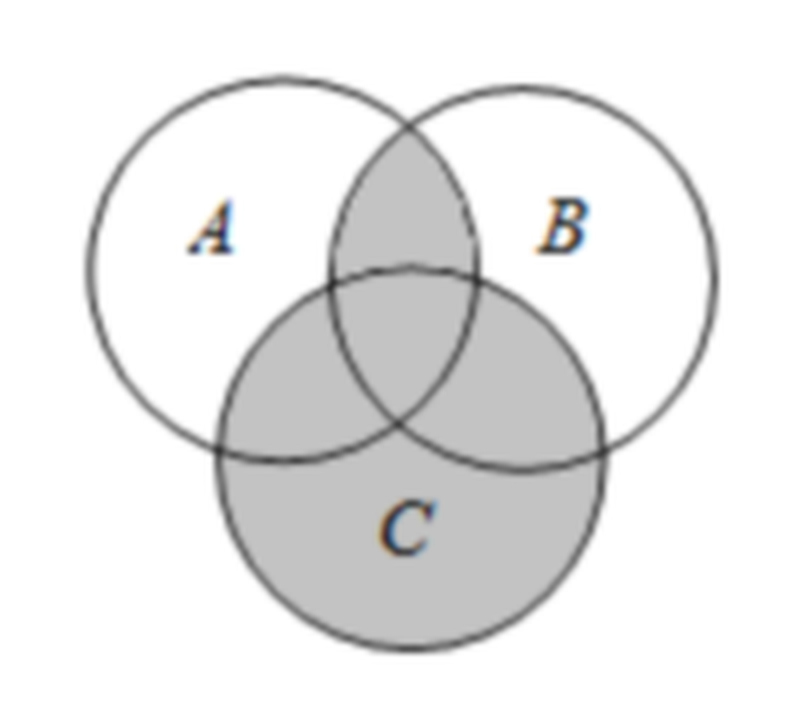
\includegraphics[width=0.30\textwidth]{figures/venn_ABcap_plus_C.png}
\end{center}

\keepwithprev
A. $(A\cup C)\cap(B\cup C)$\qquad B. $(A\cup B)\cap(A\cup C)$

C. $(A\cup B)\cap(B\cup C)$\qquad D. $(A\cup B)\cap C$

\ans{$A$}

\item 设 $f(x)=(x^2-6x+c_1)(x^2-6x+c_2)$，其中 $c_1\geqslant c_2$，集合

$M=\{x\mid f(x)=0\}=\{x_1,x_2,x_3\}\sub\Z$，则下列命题中不正确的是\mbox{（\quad）}

\keepwithprev
A. $3\in M$\qquad B. $c_2$ 可能为 $-16$

C. $c_1$ 可能为 $8$\qquad D. $M$ 中所有元素的和一定为 $9$

\ans{$C$}

\ifanswer
\solbegin
\step{若 $c_1$ 为 $8$，则 $c_2=9$，与 $c_1\geqslant c_2$ 矛盾，故选 $C$.}
\solend

\fi

\item 非空集合 $A$ 具有如下性质：①若 $x$、$y\in A$，则 $\dfrac{x}{y}\in A$；②若 $x$、$y\in A$，
则 $x+y\in A$；

由此可知：下列判断中，错误的是\mbox{（\quad）}

\keepwithprev
A. $-1\notin A$\qquad B. $\dfrac{2025}{2026}\in A$

C. 若 $x$、$y\in A$，则 $xy\in A$\qquad D. 若 $x$、$y\in A$，则 $x-y\in A$

\ans{$D$}

\ifanswer
\solbegin
\step{由题意得 $0\notin A$，$1\in A$，}
\step{对于 $A$，假设 $-1\in A$，则 $-1+1=0\in A$，矛盾，所以 $-1\notin A$，故 $A$ 正确；}
\step{对于 $B$，由 $1\in A$，得 $1+1=2\in A$，$2+1=3\in A$，$\cdots$，$2025\in A$，$2026\in A$，}
\step{所以 $\dfrac{2025}{2026}\in A$，故 $B$ 正确；}
\step{对于 $C$，因为 $1\in A$，$x\in A$，所以 $\dfrac1x\in A$，又因为 $y\in A$，
所以 $\dfrac{y}{\frac1x}=xy\in A$，}
\step{故 $C$ 正确；}
\step{对于 $D$，因为 $1\in A$，$2\in A$，若 $x=1$，$y=2$，则 $x-y=-1\notin A$，故 $D$ 错误.}
\step{故选 $D$.}
\solend

\fi

\end{enumerate}

\bigsec{三、解答题}

\begin{enumerate}
\setcounter{enumi}{13}

% 注：原卷本题题干把「$=0$」印在右花括号之外（$A=\{x\mid x^2-mx+4m-16\}=0$），
%     而其自己的【解析】印在括号之内（$A=\{x\mid x^2-mx+4m-16=0\}$）——原卷前后不一致，
%     本稿按解析与题目本意把 $=0$ 排在括号内，见文件头「排版差异」⑧。
\item 已知集合 $A=\{x\mid x^2-mx+4m-16=0\}$，$B=\{x\mid 1<x<4,x\in\N\}$，
$C=\{x\mid ax+2>0\}$，若 $A\cap B\neq\varnothing$，$A\cap C=\varnothing$，求实数 $m$ 的值以及
相应实数 $a$ 的取值范围.

\ifanswer
\solbegin
\step{集合 $A=\{x\mid x^2-mx+4m-16=0\}$，由 $\Delta=(-m)^2-4(4m-16)=(m-8)^2\geqslant0$，}
\step{所以当 $m=8$ 时，集合 $A=\{4\}$，当 $m\neq8$ 时，集合
$A=\left\{\dfrac{m-|m-8|}{2},\dfrac{m+|m-8|}{2}\right\}$，}
\step{集合 $B=\{x\mid 1<x<4,x\in\N\}$，得集合 $B=\{2,3\}$.}
\step{集合 $C=\{x\mid ax+2>0\}$，当 $a=0$ 时，集合 $C=\{x\mid x\in\R\}$，}
\step{当 $a<0$ 时，集合 $C=\left\{x\mid x<\dfrac2a\right\}$，当 $a>0$ 时，集合
$C=\left\{x\mid x>\dfrac2a\right\}$，}
\step{由 $A\cap B$ 非空得，$m=6$ 时，集合 $A=\{2,4\}$，$m=7$ 时，集合 $A=\{3,4\}$.}
\step{由 $A\cap C=\varnothing$，得 $m=6$ 或 $m=7$ 时，$a<0$ 或 $0<a<\dfrac12$ 符合要求.}
\solend

\fi

\ansspace[9]

\item 已知 $a>b>c$，$a+b+c=0$，方程 $ax^2+bx+c=0$ 的两个实根为 $x_1$、$x_2$.

\begin{enumerate}[label=(\arabic*)]
\item 证明：$-\dfrac12<\dfrac ba<1$；
% 注：此小问前加了 4pt 间距——不加时紧凑版该行的 $x_1^2$ 上标与下标恰好同箱，
%     pdftotext 抽正文会把上标当重影丢掉，make check 的正文指纹就对不上（纯抽取抖动，
%     版面与内容无差别，见 2026-09-20 入库注）。
\vspace{4pt}
\item 若 $x_1^2+x_1x_2+x_2^2=1$，求 $x_1^2-x_1x_2+x_2^2$.
\end{enumerate}

\ifanswer
\solbegin
\stepm{(1)}{因为 $a>b>c$，$a+b+c=0$，所以 $a>0$，$c<0$，$c=-a-b$，}
\step{由 $a>b$ 得 $\dfrac ba<1$ ①，由 $b>c$ 得 $b>-a-b$，即 $2b>-a$，即 $\dfrac ba>-\dfrac12$ ②，}
\step{由①②得 $-\dfrac12<\dfrac ba<1$；}
\stepm{(2)}{若 $x_1^2+x_1x_2+x_2^2=1$，则 $(x_1+x_2)^2-x_1x_2=1$，}
% 注：本行的连等式与原卷自己的结论对不上（照抄原卷、未改）——原卷印作
%     (b/a)²-b/a+1=1，则解出的应是 0 或 1；按 c=-a-b 应为 (b/a)²+b/a+1=1，
%     解得 0 或 -1（-1 因 c<0 舍去），恰与下一行「0 或 -1（舍去）」吻合。
%     详见文件头「原卷存疑」①。
\step{则 $\left(\dfrac ba\right)^2-\dfrac ca=\dfrac{b^2-ac}{a^2}
=\left(\dfrac ba\right)^2-\dfrac ba+1=1$，解得 $\dfrac ba=0$ 或 $-1$（舍去），}
\step{故 $\dfrac ba=0$，$\dfrac ca=-1$，}
\step{所以 $x_1^2-x_1x_2+x_2^2=(x_1+x_2)^2-3x_1x_2=\left(\dfrac ba\right)^2-3\times\dfrac ca=3$.}
\solend

\fi

\ansspace[6]

\item 已知方程 $x^2+px+q=0$ 与方程 $x^2+(p-3)x+2q+1=0$ 分别都有两个不相等的实根，若
他们的解集分别为 $A$、$B$，且 $A\cup B=\{1,2,5\}$，求 $p$、$q$、$A$、$B$.

\ifanswer
\solbegin
\step{两方程分别有两个不相等的实数根，而根的并集只有 $3$ 个元素，}
\step{则两方程有一公共根. 分类讨论：}
\stepm{（1）}{公共根为 $1$ 时，$x=1$ 分别代入两方程：}
\step{$\begin{cases}p+q+1=0\\ p-3+2q+1+1=0\end{cases}$，解得 $p=-3$，$q=2$，}
\step{两方程变为 $x^2-3x+2=0$，解得 $x=1$ 或 $x=2$，}
\step{$x^2-6x+5=0$ 解得 $x=1$ 或 $x=5$，满足题意.}
\stepm{（2）}{公共根为 $2$ 时，$x=2$ 分别代入两方程：}
\step{$\begin{cases}4+2p+q=0\\ 4+2p-6+2q+1=0\end{cases}$，解得 $p=-\dfrac92$，$q=5$，}
\step{第一个方程变为 $2x^2-9x+10=0$，解得 $x=2$ 或 $x=\dfrac52$，不满足题意，舍去.}
\stepm{（3）}{公共根为 $5$ 时，$x=5$ 分别代入两方程：}
\step{$\begin{cases}25+5p+q=0\\ 25+5p-15+2q+1=0\end{cases}$，解得 $p=-\dfrac{39}{5}$，$q=14$，}
\step{第一个方程变为 $5x^2-39x+70=0$，解得 $x=5$ 或 $x=\dfrac{14}{5}$，不满足题意，舍去.}
\step{综上，$p=-3$，$q=2$，$A=\{1,2\}$，$B=\{1,5\}$.}
\solend

\fi

\ansspace[8]

\item 对于集合 $A=\{a_1,a_2,\cdots,a_n\}(n\in\Z,n\geqslant3)$，其中每个元素均为正整数，如果
任意去掉其
中一个元素 $a_i(i=1,2,3\cdots,n)$ 之后，剩余的所有元素组成集合 $A_i(i=1,2,\cdots,n)$，并且
$A_i$ 都能分为两个集合 $B$ 和 $C$，满足 $B\cap C=\varnothing,B\cup C=A_i$，其中 $B$ 和 $C$
的所有元素之和相
等，就称集合 $A$ 为“可分集合”.

\begin{enumerate}[label=(\arabic*)]
\item 判断集合 $\{1,3,5,7,9,11,13\}$ 是否是“可分集合”（不必写过程）；
\item 用反证法证明：五个元素的集合 $A=\{a_1,a_2,a_3,a_4,a_5\}$ 一定不是“可分集合”；
\item 已知集合 $A=\{a_1,a_2,\cdots,a_n\}(n\in\Z,n\geqslant3)$ 是“可分集合”，求 $n$ 的最小值.
\end{enumerate}

\ifanswer
\solbegin
\stepm{(1)}{集合 $\{1,3,5,7,9,11,13\}$ 是“可分集合”；}
\stepm{(2)}{不妨设 $a_1<a_2<a_3<a_4<a_5$，}
\step{若去掉的元素为 $a_2$，将集合 $\{a_1,a_3,a_4,a_5\}$ 分成两个交集为空集的子集，}
\step{且两个子集元素之和相等，则有 $a_1+a_5=a_3+a_4$ ①，或者 $a_5=a_1+a_3+a_4$ ②；}
\step{若去掉的元素为 $a_1$，将集合 $\{a_2,a_3,a_4,a_5\}$ 分成两个交集为空集的子集，}
\step{且两个子集元素之和相等，则有 $a_2+a_5=a_3+a_4$ ③，或者 $a_5=a_2+a_3+a_4$ ④.}
\step{由①、③，得 $a_1=a_2$，矛盾；由①、④，得 $a_1=-a_2$，矛盾；}
\step{由②、③，得 $a_1=-a_2$，矛盾；由②、④，得 $a_1=a_2$ 矛盾.}
\step{因此当 $n=5$ 时，集合一定不是“可分集合”；}
\stepm{(3)}{①设集合 $A=\{a_1,a_2,\cdots,a_n\}$ 的所有元素之和为 $M$.}
\step{由题意得 $M-a_i(i=1,2,\cdots,n)$ 均为偶数，}
\step{因此 $a_i(i=1,2,\cdots,n)$ 均为奇数或偶数.}
\step{如果 $M$ 为奇数，则 $a_i(i=1,2,\cdots,n)$ 也均为奇数，}
\step{由于 $M=a_1+a_2+\cdots+a_n$，所以 $n$ 为奇数.}
\step{如果 $M$ 为偶数，则 $M-a_i(i=1,2,\cdots,n)$ 均为偶数，此时设 $a_i=2b_i$，}
\step{则 $\{b_1,b_2,\cdots,b_n\}$ 也是“可分集合”.}
\step{重复上述操作有限次，便可得各项均为奇数的“可分集合”，}
\step{此时各项之和也为奇数，则集合 $A$ 中元素个数 $n$ 为奇数.}
\step{综上所述，集合 $A$ 中元素个数为奇数.}
\step{②当 $n=3$ 时，显然任意集合 $\{a_1,a_2,a_3\}$ 不是“可分集合”.}
\step{当 $n=5$ 时，第（2）问已经证明不是“可分集合”.}
\step{当 $n=7$ 时，集合 $A=\{1,3,5,7,9,11,13\}$，}
\step{因为 $3+5+7+9=11+13$，$1+9+13=5+7+11$，$9+13=1+3+7+11$，}
\step{$1+3+5+11=7+13$，$1+9+11=3+5+13$，$3+7+9=1+5+13$，}
\step{$1+3+5+9=7+11$，则集合 $A$ 是“可分集合”，}
\step{所以集合 $A$ 中元素个数 $n$ 的最小值是 $7$.}
\solend

\fi

\ansspace*[10]

\end{enumerate}

\end{document}
"
%
% 原始材料是微信公众号图文（公众号「魔都数学加油站」连载「27学年高一 24」，2026-09-19 发布，
% 原文标题「27学年高一24——2026-2027年上海市复旦附中高一上周末作业3集合与逻辑、等式的性质」），
% 正文为 7 张 PNG 页（1080×1527，各页同尺寸）。原文本身就是一份**讲评版**——题目下方直接印出
% 【答案】或【解析】。试题文字、答案与解析均照原卷录入，未改内容。
% 卷面上的粉色斜水印「魔都数学加油站」属水印，未录入。
%
% 卷首标题：原卷印作「2026-2027 年复旦附中高一上周末作业 3」（公众号标题里有「上海市」三字，
% 卷面标题行没有，本稿照卷面），年份区间按全稿惯例排 en dash，前缀照原卷保留「年」。
%
% 与原卷的排版差异（均已在 README「说明」中交代）：
%   ① 原文自**第 3 题**起（第 1、2 题未在该文中发布），故本稿题号亦自 3 起；
%   ② 原卷本就印有「一、填空题」「二、选择题」「三、解答题」三节标题，本稿照原卷分节，
%      只把标题改排成全稿统一的「大节标题」样式；
%   ③ 原卷第 11 题的答案「A」直接印在题干末尾的括号内，第 12、13 题的括号空着、答案写在
%      解析末句「故选 C／D」里，本稿统一改为试卷版隐去、答案版以 \ans{} 给出（第 12、13 题
%      另附【解析】），使两版彻底分离；
%   ④ 原卷的集合／数集符号正体与粗体混用（第 8 题题干的 $\mathbf{R}$、第 9 题题干的
%      $\mathbf{N}$、第 12 题题干的 $\mathbf{Z}$ 为粗体，第 14 题解析的 $N$、$R$ 为斜体），
%      本稿按全稿惯例统一写作 $\R$、$\N$、$\Z$；
%   ⑤ 原卷填空的横线约两个字宽，本稿按全稿惯例统一排 \blankline[4.4em]；
%   ⑥ 第 11 题的 Venn 图原卷印在上一页末尾（第 10 题解析右侧、「二、选择题」标题旁），
%      本稿移至第 11 题题干之后；图取原卷截图、4× LANCZOS 放大
%      （figures/venn_ABcap_plus_C.png，阴影为 $A\cap B$ 的交与整个 $C$，即 $(A\cap B)\cup C$）；
%   ⑦ 原卷自印副标题「集合与逻辑、等式的性质」，本稿照录（与 高一14 同例，未改用惯例副标题）；
%   ⑧ 第 14 题题干原卷把「$=0$」印在右花括号**之外**（作
%      $A=\{x\mid x^2-mx+4m-16\}=0$），而它**自己的【解析】却印在括号之内**
%      （作 $A=\{x\mid x^2-mx+4m-16=0\}$）——原卷前后不一致；按原卷解析与题目本意，
%      本稿题干的 $=0$ 排在括号**之内**（与 高一b 第 13 题「原卷漏排 $A=$，本稿补上」同例）。
%
% 原卷存疑一处（已放大到能看清字形后核对，无法确证原意，本稿照抄原卷、未改）：
%   ① 第 15(2)【解析】的连等式印作
%      $\left(\frac ba\right)^2-\frac ca=\frac{b^2-ac}{a^2}=\left(\frac ba\right)^2-\frac ba+1=1$，
%      解得 $\frac ba=0$ 或 $-1$（舍去）——但由 $c=-a-b$ 应得 $\frac{b^2-ac}{a^2}
%      =\left(\frac ba\right)^2+\frac ba+1$（原卷把「$+\frac ba$」印成了「$-\frac ba$」）：
%      按原卷那行解出的是 $0$ 或 $1$，与其自己的结论「$0$ 或 $-1$」对不上；而按
%      $+\frac ba$ 解恰得 $0$ 或 $-1$（$-1$ 因 $c<0$ 舍去），与后文吻合。原卷显系笔误，
%      本稿照抄原卷（见源码中该处上方注释）。

\documentclass[a4paper,11pt]{article}
\usepackage{common}

\begin{document}

\examtitlest[3]{2026--2027 年复旦附中高一上周末作业 3}{集合与逻辑、等式的性质}

\bigsec{一、填空题}

\begin{enumerate}
\setcounter{enumi}{2}

\item 设 $M=\{x\mid y^2=x+2\}$，$N=\{x\mid y^2=-2x+8\}$，则 $M\cap N=$ \blankline[4.4em].

\ifanswer
\solbegin
\step{$M=[-2,+\infty)$，$N=(-\infty,4]$，则 $M\cap N=[-2,4]$.}
\solend

\fi

\item 若“$x\geqslant a$”是“$|x|\leqslant2$”的必要条件，则实数 $a$ 的取值集合是 \blankline[4.4em].

\ans{$(-\infty,-2]$}

\item 某校一年级的 $200$ 人中，爱好数学的有 $95$ 人，爱好体育的有 $156$ 人，则数学体育都爱好
的至少有 \blankline[4.4em] 人.

\ifanswer
\solbegin
\step{数学体育都爱好的至少有 $95+156-200=51$ 人.}
\solend

\fi

\item 已知 $x$ 为实数，且 $x^2+\dfrac{1}{x^2}=3$，则 $x^3+\dfrac{1}{x^3}$ 的值是 \blankline[4.4em].

\ifanswer
\solbegin
\step{因为 $x^2+\dfrac{1}{x^2}=\left(x+\dfrac1x\right)^2-2=3$，所以 $x+\dfrac1x=\pm\sqrt5$，}
\step{所以 $x^3+\dfrac{1}{x^3}=\left(x+\dfrac1x\right)\left(x^2-1+\dfrac{1}{x^2}\right)=\pm2\sqrt5$.}
\solend

\fi

\item 非空集合 $A=\{x\mid a+1\leqslant x<2a-1\}$，$B=\{x\mid-2\leqslant x\leqslant5\}$，
若 $A\sub(A\cap B)$，则 $a$ 的取值范围是 \blankline[4.4em].

\ifanswer
\solbegin
\step{当 $a+1<2a-1$，即 $a>2$ 时，$A\neq\varnothing$，由 $A\sub(A\cap B)$ 得 $A\sub B$，}
\step{得 $\begin{cases}a+1\geqslant-2\\ 2a-1\leqslant5\end{cases}$，解得 $-3\leqslant a\leqslant3$，所以 $2<a\leqslant3$.}
\solend

\fi

\item 已知集合 $\{x\mid(x-1)(x^2-x+a)=0,x\in\R\}$ 中的所有元素之和为 $1$，则实数 $a$ 的取值范
围是 \blankline[4.4em].

\ifanswer
\solbegin
\step{令 $x-1=0$，得 $x=1$，}
\stepm{①}{若 $x^2-x+a=0$ 无实数根，则 $\Delta=1-4a<0$，解得 $a>\dfrac14$，}
\step{此时集合只有元素 $1$，符合题意；}
\stepm{②}{若 $x^2-x+a=0$ 有两个相等的实数根，则 $\Delta=1-4a=0$，解得 $a=\dfrac14$，}
\step{此时方程为 $x^2-x+\dfrac14=0$，解得 $x=\dfrac12$，此时集合为 $\left\{1,\dfrac12\right\}$，不合题意；}
\stepm{③}{若 $x^2-x+a=0$ 有两个不相等的实数根，则 $\Delta=1-4a>0$，解得 $a<\dfrac14$，}
\step{设方程 $x^2-x+a=0$ 的两个实根分别为 $x_1,x_2$，则 $x_1+x_2=1$，}
\step{若 $x_1\neq1,x_2\neq1$，则集合为 $\{1,x_1,x_2\}$，不合题意，}
\step{若 $x_1=1$，则 $x_2=0$，此时集合为 $\{1,0\}$，符合题意，所以 $a=x_1x_2=0$，}
\step{综上所述，实数 $a$ 的取值范围是 $\{0\}\cup\left(\dfrac14,+\infty\right)$.}
\solend

\fi

\item 集合 $A=\{m\mid m=2k,k\in\N,1\leqslant k\leqslant50\}$，
$B=\{n\mid n=i+j,i<j,i\in A,j\in A\}$，则 $B$ 中元素的个数是 \blankline[4.4em].

\ifanswer
\solbegin
\step{$B$ 中最小元素是 $6$，最大元素是 $198$，则 $B$ 中元素的个数是 $\dfrac{198-6}{2}+1=97$.}
\solend

\fi

\item 关于 $(x,y,z)$ 的方程组
$\begin{cases}x^2+y^2+25z^2=6zx+8yz\\ 3x^2+2y^2+z^2=240\end{cases}$ 的解集为 \blankline[4.4em].

\ifanswer
\solbegin
\step{由上式得 $(x^2-6xz+9z^2)+(y^2-8yz+16z^2)=0$，}
\step{则 $(x-3z)^2+(y-4z)^2=0$，}
\step{所以 $(x,y,z)=(3t,4t,t)$，$t$ 为实数，代入下式中 $27\cdot t^2+32t^2+t^2=60t^2=240$，}
\step{则 $t^2=4$，$t=\pm2$，所以 $(x,y,z)=(6,8,2),(-6,-8,-2)$.}
\solend

\fi

\end{enumerate}

\bigsec{二、选择题}

\begin{enumerate}
\setcounter{enumi}{10}

\item 下列表示图形中的阴影部分的是\mbox{（\quad）}

\begin{center}
% 图取原卷截图、4× LANCZOS 放大（原卷把图印在上一页末尾，本稿移至此处，见文件头⑥）。
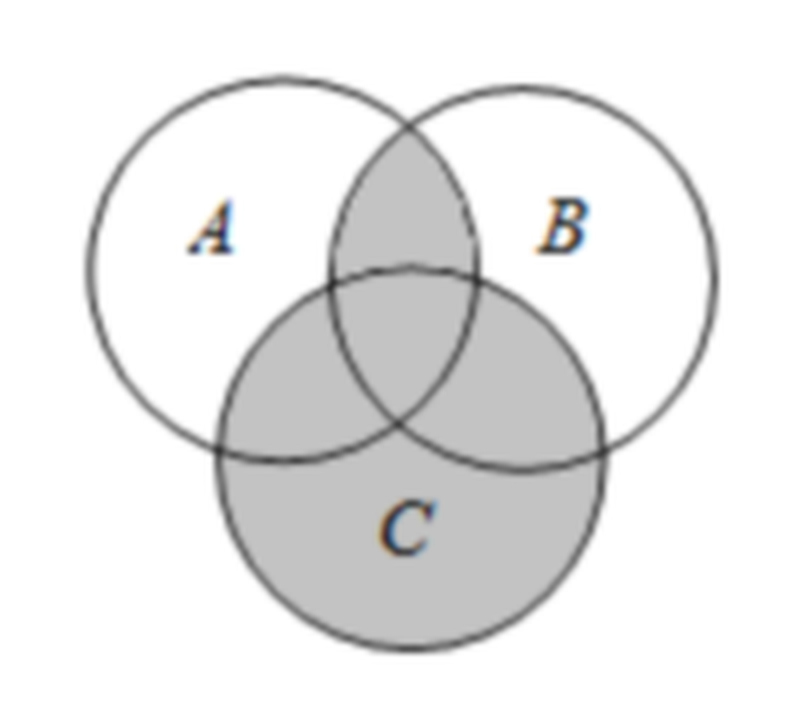
\includegraphics[width=0.30\textwidth]{figures/venn_ABcap_plus_C.png}
\end{center}

\keepwithprev
A. $(A\cup C)\cap(B\cup C)$\qquad B. $(A\cup B)\cap(A\cup C)$

C. $(A\cup B)\cap(B\cup C)$\qquad D. $(A\cup B)\cap C$

\ans{$A$}

\item 设 $f(x)=(x^2-6x+c_1)(x^2-6x+c_2)$，其中 $c_1\geqslant c_2$，集合

$M=\{x\mid f(x)=0\}=\{x_1,x_2,x_3\}\sub\Z$，则下列命题中不正确的是\mbox{（\quad）}

\keepwithprev
A. $3\in M$\qquad B. $c_2$ 可能为 $-16$

C. $c_1$ 可能为 $8$\qquad D. $M$ 中所有元素的和一定为 $9$

\ans{$C$}

\ifanswer
\solbegin
\step{若 $c_1$ 为 $8$，则 $c_2=9$，与 $c_1\geqslant c_2$ 矛盾，故选 $C$.}
\solend

\fi

\item 非空集合 $A$ 具有如下性质：①若 $x$、$y\in A$，则 $\dfrac{x}{y}\in A$；②若 $x$、$y\in A$，
则 $x+y\in A$；

由此可知：下列判断中，错误的是\mbox{（\quad）}

\keepwithprev
A. $-1\notin A$\qquad B. $\dfrac{2025}{2026}\in A$

C. 若 $x$、$y\in A$，则 $xy\in A$\qquad D. 若 $x$、$y\in A$，则 $x-y\in A$

\ans{$D$}

\ifanswer
\solbegin
\step{由题意得 $0\notin A$，$1\in A$，}
\step{对于 $A$，假设 $-1\in A$，则 $-1+1=0\in A$，矛盾，所以 $-1\notin A$，故 $A$ 正确；}
\step{对于 $B$，由 $1\in A$，得 $1+1=2\in A$，$2+1=3\in A$，$\cdots$，$2025\in A$，$2026\in A$，}
\step{所以 $\dfrac{2025}{2026}\in A$，故 $B$ 正确；}
\step{对于 $C$，因为 $1\in A$，$x\in A$，所以 $\dfrac1x\in A$，又因为 $y\in A$，
所以 $\dfrac{y}{\frac1x}=xy\in A$，}
\step{故 $C$ 正确；}
\step{对于 $D$，因为 $1\in A$，$2\in A$，若 $x=1$，$y=2$，则 $x-y=-1\notin A$，故 $D$ 错误.}
\step{故选 $D$.}
\solend

\fi

\end{enumerate}

\bigsec{三、解答题}

\begin{enumerate}
\setcounter{enumi}{13}

% 注：原卷本题题干把「$=0$」印在右花括号之外（$A=\{x\mid x^2-mx+4m-16\}=0$），
%     而其自己的【解析】印在括号之内（$A=\{x\mid x^2-mx+4m-16=0\}$）——原卷前后不一致，
%     本稿按解析与题目本意把 $=0$ 排在括号内，见文件头「排版差异」⑧。
\item 已知集合 $A=\{x\mid x^2-mx+4m-16=0\}$，$B=\{x\mid 1<x<4,x\in\N\}$，
$C=\{x\mid ax+2>0\}$，若 $A\cap B\neq\varnothing$，$A\cap C=\varnothing$，求实数 $m$ 的值以及
相应实数 $a$ 的取值范围.

\ifanswer
\solbegin
\step{集合 $A=\{x\mid x^2-mx+4m-16=0\}$，由 $\Delta=(-m)^2-4(4m-16)=(m-8)^2\geqslant0$，}
\step{所以当 $m=8$ 时，集合 $A=\{4\}$，当 $m\neq8$ 时，集合
$A=\left\{\dfrac{m-|m-8|}{2},\dfrac{m+|m-8|}{2}\right\}$，}
\step{集合 $B=\{x\mid 1<x<4,x\in\N\}$，得集合 $B=\{2,3\}$.}
\step{集合 $C=\{x\mid ax+2>0\}$，当 $a=0$ 时，集合 $C=\{x\mid x\in\R\}$，}
\step{当 $a<0$ 时，集合 $C=\left\{x\mid x<\dfrac2a\right\}$，当 $a>0$ 时，集合
$C=\left\{x\mid x>\dfrac2a\right\}$，}
\step{由 $A\cap B$ 非空得，$m=6$ 时，集合 $A=\{2,4\}$，$m=7$ 时，集合 $A=\{3,4\}$.}
\step{由 $A\cap C=\varnothing$，得 $m=6$ 或 $m=7$ 时，$a<0$ 或 $0<a<\dfrac12$ 符合要求.}
\solend

\fi

\ansspace[9]

\item 已知 $a>b>c$，$a+b+c=0$，方程 $ax^2+bx+c=0$ 的两个实根为 $x_1$、$x_2$.

\begin{enumerate}[label=(\arabic*)]
\item 证明：$-\dfrac12<\dfrac ba<1$；
% 注：此小问前加了 4pt 间距——不加时紧凑版该行的 $x_1^2$ 上标与下标恰好同箱，
%     pdftotext 抽正文会把上标当重影丢掉，make check 的正文指纹就对不上（纯抽取抖动，
%     版面与内容无差别，见 2026-09-20 入库注）。
\vspace{4pt}
\item 若 $x_1^2+x_1x_2+x_2^2=1$，求 $x_1^2-x_1x_2+x_2^2$.
\end{enumerate}

\ifanswer
\solbegin
\stepm{(1)}{因为 $a>b>c$，$a+b+c=0$，所以 $a>0$，$c<0$，$c=-a-b$，}
\step{由 $a>b$ 得 $\dfrac ba<1$ ①，由 $b>c$ 得 $b>-a-b$，即 $2b>-a$，即 $\dfrac ba>-\dfrac12$ ②，}
\step{由①②得 $-\dfrac12<\dfrac ba<1$；}
\stepm{(2)}{若 $x_1^2+x_1x_2+x_2^2=1$，则 $(x_1+x_2)^2-x_1x_2=1$，}
% 注：本行的连等式与原卷自己的结论对不上（照抄原卷、未改）——原卷印作
%     (b/a)²-b/a+1=1，则解出的应是 0 或 1；按 c=-a-b 应为 (b/a)²+b/a+1=1，
%     解得 0 或 -1（-1 因 c<0 舍去），恰与下一行「0 或 -1（舍去）」吻合。
%     详见文件头「原卷存疑」①。
\step{则 $\left(\dfrac ba\right)^2-\dfrac ca=\dfrac{b^2-ac}{a^2}
=\left(\dfrac ba\right)^2-\dfrac ba+1=1$，解得 $\dfrac ba=0$ 或 $-1$（舍去），}
\step{故 $\dfrac ba=0$，$\dfrac ca=-1$，}
\step{所以 $x_1^2-x_1x_2+x_2^2=(x_1+x_2)^2-3x_1x_2=\left(\dfrac ba\right)^2-3\times\dfrac ca=3$.}
\solend

\fi

\ansspace[6]

\item 已知方程 $x^2+px+q=0$ 与方程 $x^2+(p-3)x+2q+1=0$ 分别都有两个不相等的实根，若
他们的解集分别为 $A$、$B$，且 $A\cup B=\{1,2,5\}$，求 $p$、$q$、$A$、$B$.

\ifanswer
\solbegin
\step{两方程分别有两个不相等的实数根，而根的并集只有 $3$ 个元素，}
\step{则两方程有一公共根. 分类讨论：}
\stepm{（1）}{公共根为 $1$ 时，$x=1$ 分别代入两方程：}
\step{$\begin{cases}p+q+1=0\\ p-3+2q+1+1=0\end{cases}$，解得 $p=-3$，$q=2$，}
\step{两方程变为 $x^2-3x+2=0$，解得 $x=1$ 或 $x=2$，}
\step{$x^2-6x+5=0$ 解得 $x=1$ 或 $x=5$，满足题意.}
\stepm{（2）}{公共根为 $2$ 时，$x=2$ 分别代入两方程：}
\step{$\begin{cases}4+2p+q=0\\ 4+2p-6+2q+1=0\end{cases}$，解得 $p=-\dfrac92$，$q=5$，}
\step{第一个方程变为 $2x^2-9x+10=0$，解得 $x=2$ 或 $x=\dfrac52$，不满足题意，舍去.}
\stepm{（3）}{公共根为 $5$ 时，$x=5$ 分别代入两方程：}
\step{$\begin{cases}25+5p+q=0\\ 25+5p-15+2q+1=0\end{cases}$，解得 $p=-\dfrac{39}{5}$，$q=14$，}
\step{第一个方程变为 $5x^2-39x+70=0$，解得 $x=5$ 或 $x=\dfrac{14}{5}$，不满足题意，舍去.}
\step{综上，$p=-3$，$q=2$，$A=\{1,2\}$，$B=\{1,5\}$.}
\solend

\fi

\ansspace[8]

\item 对于集合 $A=\{a_1,a_2,\cdots,a_n\}(n\in\Z,n\geqslant3)$，其中每个元素均为正整数，如果
任意去掉其
中一个元素 $a_i(i=1,2,3\cdots,n)$ 之后，剩余的所有元素组成集合 $A_i(i=1,2,\cdots,n)$，并且
$A_i$ 都能分为两个集合 $B$ 和 $C$，满足 $B\cap C=\varnothing,B\cup C=A_i$，其中 $B$ 和 $C$
的所有元素之和相
等，就称集合 $A$ 为“可分集合”.

\begin{enumerate}[label=(\arabic*)]
\item 判断集合 $\{1,3,5,7,9,11,13\}$ 是否是“可分集合”（不必写过程）；
\item 用反证法证明：五个元素的集合 $A=\{a_1,a_2,a_3,a_4,a_5\}$ 一定不是“可分集合”；
\item 已知集合 $A=\{a_1,a_2,\cdots,a_n\}(n\in\Z,n\geqslant3)$ 是“可分集合”，求 $n$ 的最小值.
\end{enumerate}

\ifanswer
\solbegin
\stepm{(1)}{集合 $\{1,3,5,7,9,11,13\}$ 是“可分集合”；}
\stepm{(2)}{不妨设 $a_1<a_2<a_3<a_4<a_5$，}
\step{若去掉的元素为 $a_2$，将集合 $\{a_1,a_3,a_4,a_5\}$ 分成两个交集为空集的子集，}
\step{且两个子集元素之和相等，则有 $a_1+a_5=a_3+a_4$ ①，或者 $a_5=a_1+a_3+a_4$ ②；}
\step{若去掉的元素为 $a_1$，将集合 $\{a_2,a_3,a_4,a_5\}$ 分成两个交集为空集的子集，}
\step{且两个子集元素之和相等，则有 $a_2+a_5=a_3+a_4$ ③，或者 $a_5=a_2+a_3+a_4$ ④.}
\step{由①、③，得 $a_1=a_2$，矛盾；由①、④，得 $a_1=-a_2$，矛盾；}
\step{由②、③，得 $a_1=-a_2$，矛盾；由②、④，得 $a_1=a_2$ 矛盾.}
\step{因此当 $n=5$ 时，集合一定不是“可分集合”；}
\stepm{(3)}{①设集合 $A=\{a_1,a_2,\cdots,a_n\}$ 的所有元素之和为 $M$.}
\step{由题意得 $M-a_i(i=1,2,\cdots,n)$ 均为偶数，}
\step{因此 $a_i(i=1,2,\cdots,n)$ 均为奇数或偶数.}
\step{如果 $M$ 为奇数，则 $a_i(i=1,2,\cdots,n)$ 也均为奇数，}
\step{由于 $M=a_1+a_2+\cdots+a_n$，所以 $n$ 为奇数.}
\step{如果 $M$ 为偶数，则 $M-a_i(i=1,2,\cdots,n)$ 均为偶数，此时设 $a_i=2b_i$，}
\step{则 $\{b_1,b_2,\cdots,b_n\}$ 也是“可分集合”.}
\step{重复上述操作有限次，便可得各项均为奇数的“可分集合”，}
\step{此时各项之和也为奇数，则集合 $A$ 中元素个数 $n$ 为奇数.}
\step{综上所述，集合 $A$ 中元素个数为奇数.}
\step{②当 $n=3$ 时，显然任意集合 $\{a_1,a_2,a_3\}$ 不是“可分集合”.}
\step{当 $n=5$ 时，第（2）问已经证明不是“可分集合”.}
\step{当 $n=7$ 时，集合 $A=\{1,3,5,7,9,11,13\}$，}
\step{因为 $3+5+7+9=11+13$，$1+9+13=5+7+11$，$9+13=1+3+7+11$，}
\step{$1+3+5+11=7+13$，$1+9+11=3+5+13$，$3+7+9=1+5+13$，}
\step{$1+3+5+9=7+11$，则集合 $A$ 是“可分集合”，}
\step{所以集合 $A$ 中元素个数 $n$ 的最小值是 $7$.}
\solend

\fi

\ansspace*[10]

\end{enumerate}

\end{document}
"
% 紧凑版：xelatex "\def\iscompact{1}% 高一24_复旦附中_周末作业3.tex
%   —— 高一上数学「2026-2027 年复旦附中高一上周末作业 3」（试卷版/答案版）
% 试卷版：xelatex 高一24_复旦附中_周末作业3.tex
% 答案版：xelatex "\def\isanswer{1}% 高一24_复旦附中_周末作业3.tex
%   —— 高一上数学「2026-2027 年复旦附中高一上周末作业 3」（试卷版/答案版）
% 试卷版：xelatex 高一24_复旦附中_周末作业3.tex
% 答案版：xelatex "\def\isanswer{1}% 高一24_复旦附中_周末作业3.tex
%   —— 高一上数学「2026-2027 年复旦附中高一上周末作业 3」（试卷版/答案版）
% 试卷版：xelatex 高一24_复旦附中_周末作业3.tex
% 答案版：xelatex "\def\isanswer{1}\input{高一24_复旦附中_周末作业3.tex}"
% 紧凑版：xelatex "\def\iscompact{1}\input{高一24_复旦附中_周末作业3.tex}"
%
% 原始材料是微信公众号图文（公众号「魔都数学加油站」连载「27学年高一 24」，2026-09-19 发布，
% 原文标题「27学年高一24——2026-2027年上海市复旦附中高一上周末作业3集合与逻辑、等式的性质」），
% 正文为 7 张 PNG 页（1080×1527，各页同尺寸）。原文本身就是一份**讲评版**——题目下方直接印出
% 【答案】或【解析】。试题文字、答案与解析均照原卷录入，未改内容。
% 卷面上的粉色斜水印「魔都数学加油站」属水印，未录入。
%
% 卷首标题：原卷印作「2026-2027 年复旦附中高一上周末作业 3」（公众号标题里有「上海市」三字，
% 卷面标题行没有，本稿照卷面），年份区间按全稿惯例排 en dash，前缀照原卷保留「年」。
%
% 与原卷的排版差异（均已在 README「说明」中交代）：
%   ① 原文自**第 3 题**起（第 1、2 题未在该文中发布），故本稿题号亦自 3 起；
%   ② 原卷本就印有「一、填空题」「二、选择题」「三、解答题」三节标题，本稿照原卷分节，
%      只把标题改排成全稿统一的「大节标题」样式；
%   ③ 原卷第 11 题的答案「A」直接印在题干末尾的括号内，第 12、13 题的括号空着、答案写在
%      解析末句「故选 C／D」里，本稿统一改为试卷版隐去、答案版以 \ans{} 给出（第 12、13 题
%      另附【解析】），使两版彻底分离；
%   ④ 原卷的集合／数集符号正体与粗体混用（第 8 题题干的 $\mathbf{R}$、第 9 题题干的
%      $\mathbf{N}$、第 12 题题干的 $\mathbf{Z}$ 为粗体，第 14 题解析的 $N$、$R$ 为斜体），
%      本稿按全稿惯例统一写作 $\R$、$\N$、$\Z$；
%   ⑤ 原卷填空的横线约两个字宽，本稿按全稿惯例统一排 \blankline[4.4em]；
%   ⑥ 第 11 题的 Venn 图原卷印在上一页末尾（第 10 题解析右侧、「二、选择题」标题旁），
%      本稿移至第 11 题题干之后；图取原卷截图、4× LANCZOS 放大
%      （figures/venn_ABcap_plus_C.png，阴影为 $A\cap B$ 的交与整个 $C$，即 $(A\cap B)\cup C$）；
%   ⑦ 原卷自印副标题「集合与逻辑、等式的性质」，本稿照录（与 高一14 同例，未改用惯例副标题）；
%   ⑧ 第 14 题题干原卷把「$=0$」印在右花括号**之外**（作
%      $A=\{x\mid x^2-mx+4m-16\}=0$），而它**自己的【解析】却印在括号之内**
%      （作 $A=\{x\mid x^2-mx+4m-16=0\}$）——原卷前后不一致；按原卷解析与题目本意，
%      本稿题干的 $=0$ 排在括号**之内**（与 高一b 第 13 题「原卷漏排 $A=$，本稿补上」同例）。
%
% 原卷存疑一处（已放大到能看清字形后核对，无法确证原意，本稿照抄原卷、未改）：
%   ① 第 15(2)【解析】的连等式印作
%      $\left(\frac ba\right)^2-\frac ca=\frac{b^2-ac}{a^2}=\left(\frac ba\right)^2-\frac ba+1=1$，
%      解得 $\frac ba=0$ 或 $-1$（舍去）——但由 $c=-a-b$ 应得 $\frac{b^2-ac}{a^2}
%      =\left(\frac ba\right)^2+\frac ba+1$（原卷把「$+\frac ba$」印成了「$-\frac ba$」）：
%      按原卷那行解出的是 $0$ 或 $1$，与其自己的结论「$0$ 或 $-1$」对不上；而按
%      $+\frac ba$ 解恰得 $0$ 或 $-1$（$-1$ 因 $c<0$ 舍去），与后文吻合。原卷显系笔误，
%      本稿照抄原卷（见源码中该处上方注释）。

\documentclass[a4paper,11pt]{article}
\usepackage{common}

\begin{document}

\examtitlest[3]{2026--2027 年复旦附中高一上周末作业 3}{集合与逻辑、等式的性质}

\bigsec{一、填空题}

\begin{enumerate}
\setcounter{enumi}{2}

\item 设 $M=\{x\mid y^2=x+2\}$，$N=\{x\mid y^2=-2x+8\}$，则 $M\cap N=$ \blankline[4.4em].

\ifanswer
\solbegin
\step{$M=[-2,+\infty)$，$N=(-\infty,4]$，则 $M\cap N=[-2,4]$.}
\solend

\fi

\item 若“$x\geqslant a$”是“$|x|\leqslant2$”的必要条件，则实数 $a$ 的取值集合是 \blankline[4.4em].

\ans{$(-\infty,-2]$}

\item 某校一年级的 $200$ 人中，爱好数学的有 $95$ 人，爱好体育的有 $156$ 人，则数学体育都爱好
的至少有 \blankline[4.4em] 人.

\ifanswer
\solbegin
\step{数学体育都爱好的至少有 $95+156-200=51$ 人.}
\solend

\fi

\item 已知 $x$ 为实数，且 $x^2+\dfrac{1}{x^2}=3$，则 $x^3+\dfrac{1}{x^3}$ 的值是 \blankline[4.4em].

\ifanswer
\solbegin
\step{因为 $x^2+\dfrac{1}{x^2}=\left(x+\dfrac1x\right)^2-2=3$，所以 $x+\dfrac1x=\pm\sqrt5$，}
\step{所以 $x^3+\dfrac{1}{x^3}=\left(x+\dfrac1x\right)\left(x^2-1+\dfrac{1}{x^2}\right)=\pm2\sqrt5$.}
\solend

\fi

\item 非空集合 $A=\{x\mid a+1\leqslant x<2a-1\}$，$B=\{x\mid-2\leqslant x\leqslant5\}$，
若 $A\sub(A\cap B)$，则 $a$ 的取值范围是 \blankline[4.4em].

\ifanswer
\solbegin
\step{当 $a+1<2a-1$，即 $a>2$ 时，$A\neq\varnothing$，由 $A\sub(A\cap B)$ 得 $A\sub B$，}
\step{得 $\begin{cases}a+1\geqslant-2\\ 2a-1\leqslant5\end{cases}$，解得 $-3\leqslant a\leqslant3$，所以 $2<a\leqslant3$.}
\solend

\fi

\item 已知集合 $\{x\mid(x-1)(x^2-x+a)=0,x\in\R\}$ 中的所有元素之和为 $1$，则实数 $a$ 的取值范
围是 \blankline[4.4em].

\ifanswer
\solbegin
\step{令 $x-1=0$，得 $x=1$，}
\stepm{①}{若 $x^2-x+a=0$ 无实数根，则 $\Delta=1-4a<0$，解得 $a>\dfrac14$，}
\step{此时集合只有元素 $1$，符合题意；}
\stepm{②}{若 $x^2-x+a=0$ 有两个相等的实数根，则 $\Delta=1-4a=0$，解得 $a=\dfrac14$，}
\step{此时方程为 $x^2-x+\dfrac14=0$，解得 $x=\dfrac12$，此时集合为 $\left\{1,\dfrac12\right\}$，不合题意；}
\stepm{③}{若 $x^2-x+a=0$ 有两个不相等的实数根，则 $\Delta=1-4a>0$，解得 $a<\dfrac14$，}
\step{设方程 $x^2-x+a=0$ 的两个实根分别为 $x_1,x_2$，则 $x_1+x_2=1$，}
\step{若 $x_1\neq1,x_2\neq1$，则集合为 $\{1,x_1,x_2\}$，不合题意，}
\step{若 $x_1=1$，则 $x_2=0$，此时集合为 $\{1,0\}$，符合题意，所以 $a=x_1x_2=0$，}
\step{综上所述，实数 $a$ 的取值范围是 $\{0\}\cup\left(\dfrac14,+\infty\right)$.}
\solend

\fi

\item 集合 $A=\{m\mid m=2k,k\in\N,1\leqslant k\leqslant50\}$，
$B=\{n\mid n=i+j,i<j,i\in A,j\in A\}$，则 $B$ 中元素的个数是 \blankline[4.4em].

\ifanswer
\solbegin
\step{$B$ 中最小元素是 $6$，最大元素是 $198$，则 $B$ 中元素的个数是 $\dfrac{198-6}{2}+1=97$.}
\solend

\fi

\item 关于 $(x,y,z)$ 的方程组
$\begin{cases}x^2+y^2+25z^2=6zx+8yz\\ 3x^2+2y^2+z^2=240\end{cases}$ 的解集为 \blankline[4.4em].

\ifanswer
\solbegin
\step{由上式得 $(x^2-6xz+9z^2)+(y^2-8yz+16z^2)=0$，}
\step{则 $(x-3z)^2+(y-4z)^2=0$，}
\step{所以 $(x,y,z)=(3t,4t,t)$，$t$ 为实数，代入下式中 $27\cdot t^2+32t^2+t^2=60t^2=240$，}
\step{则 $t^2=4$，$t=\pm2$，所以 $(x,y,z)=(6,8,2),(-6,-8,-2)$.}
\solend

\fi

\end{enumerate}

\bigsec{二、选择题}

\begin{enumerate}
\setcounter{enumi}{10}

\item 下列表示图形中的阴影部分的是\mbox{（\quad）}

\begin{center}
% 图取原卷截图、4× LANCZOS 放大（原卷把图印在上一页末尾，本稿移至此处，见文件头⑥）。
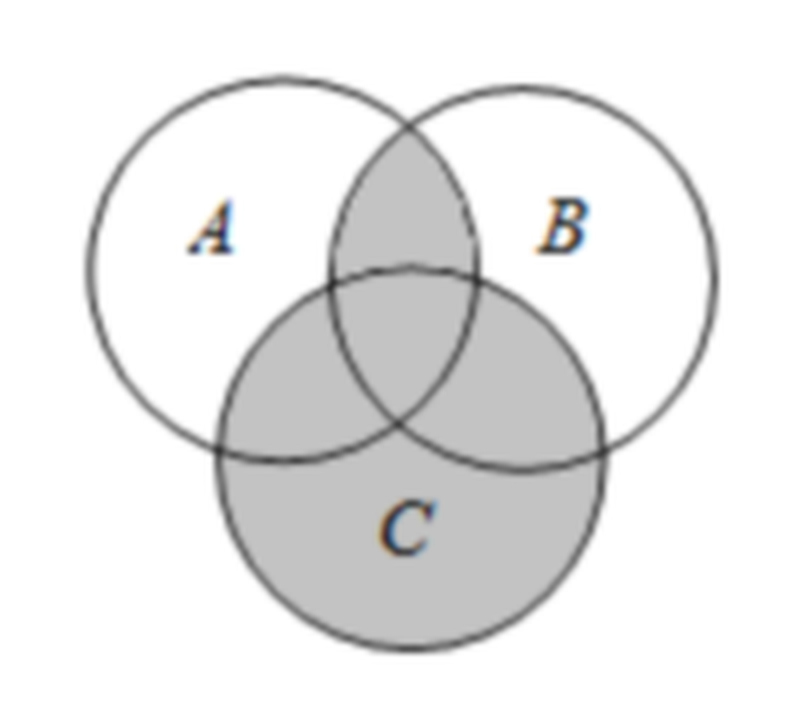
\includegraphics[width=0.30\textwidth]{figures/venn_ABcap_plus_C.png}
\end{center}

\keepwithprev
A. $(A\cup C)\cap(B\cup C)$\qquad B. $(A\cup B)\cap(A\cup C)$

C. $(A\cup B)\cap(B\cup C)$\qquad D. $(A\cup B)\cap C$

\ans{$A$}

\item 设 $f(x)=(x^2-6x+c_1)(x^2-6x+c_2)$，其中 $c_1\geqslant c_2$，集合

$M=\{x\mid f(x)=0\}=\{x_1,x_2,x_3\}\sub\Z$，则下列命题中不正确的是\mbox{（\quad）}

\keepwithprev
A. $3\in M$\qquad B. $c_2$ 可能为 $-16$

C. $c_1$ 可能为 $8$\qquad D. $M$ 中所有元素的和一定为 $9$

\ans{$C$}

\ifanswer
\solbegin
\step{若 $c_1$ 为 $8$，则 $c_2=9$，与 $c_1\geqslant c_2$ 矛盾，故选 $C$.}
\solend

\fi

\item 非空集合 $A$ 具有如下性质：①若 $x$、$y\in A$，则 $\dfrac{x}{y}\in A$；②若 $x$、$y\in A$，
则 $x+y\in A$；

由此可知：下列判断中，错误的是\mbox{（\quad）}

\keepwithprev
A. $-1\notin A$\qquad B. $\dfrac{2025}{2026}\in A$

C. 若 $x$、$y\in A$，则 $xy\in A$\qquad D. 若 $x$、$y\in A$，则 $x-y\in A$

\ans{$D$}

\ifanswer
\solbegin
\step{由题意得 $0\notin A$，$1\in A$，}
\step{对于 $A$，假设 $-1\in A$，则 $-1+1=0\in A$，矛盾，所以 $-1\notin A$，故 $A$ 正确；}
\step{对于 $B$，由 $1\in A$，得 $1+1=2\in A$，$2+1=3\in A$，$\cdots$，$2025\in A$，$2026\in A$，}
\step{所以 $\dfrac{2025}{2026}\in A$，故 $B$ 正确；}
\step{对于 $C$，因为 $1\in A$，$x\in A$，所以 $\dfrac1x\in A$，又因为 $y\in A$，
所以 $\dfrac{y}{\frac1x}=xy\in A$，}
\step{故 $C$ 正确；}
\step{对于 $D$，因为 $1\in A$，$2\in A$，若 $x=1$，$y=2$，则 $x-y=-1\notin A$，故 $D$ 错误.}
\step{故选 $D$.}
\solend

\fi

\end{enumerate}

\bigsec{三、解答题}

\begin{enumerate}
\setcounter{enumi}{13}

% 注：原卷本题题干把「$=0$」印在右花括号之外（$A=\{x\mid x^2-mx+4m-16\}=0$），
%     而其自己的【解析】印在括号之内（$A=\{x\mid x^2-mx+4m-16=0\}$）——原卷前后不一致，
%     本稿按解析与题目本意把 $=0$ 排在括号内，见文件头「排版差异」⑧。
\item 已知集合 $A=\{x\mid x^2-mx+4m-16=0\}$，$B=\{x\mid 1<x<4,x\in\N\}$，
$C=\{x\mid ax+2>0\}$，若 $A\cap B\neq\varnothing$，$A\cap C=\varnothing$，求实数 $m$ 的值以及
相应实数 $a$ 的取值范围.

\ifanswer
\solbegin
\step{集合 $A=\{x\mid x^2-mx+4m-16=0\}$，由 $\Delta=(-m)^2-4(4m-16)=(m-8)^2\geqslant0$，}
\step{所以当 $m=8$ 时，集合 $A=\{4\}$，当 $m\neq8$ 时，集合
$A=\left\{\dfrac{m-|m-8|}{2},\dfrac{m+|m-8|}{2}\right\}$，}
\step{集合 $B=\{x\mid 1<x<4,x\in\N\}$，得集合 $B=\{2,3\}$.}
\step{集合 $C=\{x\mid ax+2>0\}$，当 $a=0$ 时，集合 $C=\{x\mid x\in\R\}$，}
\step{当 $a<0$ 时，集合 $C=\left\{x\mid x<\dfrac2a\right\}$，当 $a>0$ 时，集合
$C=\left\{x\mid x>\dfrac2a\right\}$，}
\step{由 $A\cap B$ 非空得，$m=6$ 时，集合 $A=\{2,4\}$，$m=7$ 时，集合 $A=\{3,4\}$.}
\step{由 $A\cap C=\varnothing$，得 $m=6$ 或 $m=7$ 时，$a<0$ 或 $0<a<\dfrac12$ 符合要求.}
\solend

\fi

\ansspace[9]

\item 已知 $a>b>c$，$a+b+c=0$，方程 $ax^2+bx+c=0$ 的两个实根为 $x_1$、$x_2$.

\begin{enumerate}[label=(\arabic*)]
\item 证明：$-\dfrac12<\dfrac ba<1$；
% 注：此小问前加了 4pt 间距——不加时紧凑版该行的 $x_1^2$ 上标与下标恰好同箱，
%     pdftotext 抽正文会把上标当重影丢掉，make check 的正文指纹就对不上（纯抽取抖动，
%     版面与内容无差别，见 2026-09-20 入库注）。
\vspace{4pt}
\item 若 $x_1^2+x_1x_2+x_2^2=1$，求 $x_1^2-x_1x_2+x_2^2$.
\end{enumerate}

\ifanswer
\solbegin
\stepm{(1)}{因为 $a>b>c$，$a+b+c=0$，所以 $a>0$，$c<0$，$c=-a-b$，}
\step{由 $a>b$ 得 $\dfrac ba<1$ ①，由 $b>c$ 得 $b>-a-b$，即 $2b>-a$，即 $\dfrac ba>-\dfrac12$ ②，}
\step{由①②得 $-\dfrac12<\dfrac ba<1$；}
\stepm{(2)}{若 $x_1^2+x_1x_2+x_2^2=1$，则 $(x_1+x_2)^2-x_1x_2=1$，}
% 注：本行的连等式与原卷自己的结论对不上（照抄原卷、未改）——原卷印作
%     (b/a)²-b/a+1=1，则解出的应是 0 或 1；按 c=-a-b 应为 (b/a)²+b/a+1=1，
%     解得 0 或 -1（-1 因 c<0 舍去），恰与下一行「0 或 -1（舍去）」吻合。
%     详见文件头「原卷存疑」①。
\step{则 $\left(\dfrac ba\right)^2-\dfrac ca=\dfrac{b^2-ac}{a^2}
=\left(\dfrac ba\right)^2-\dfrac ba+1=1$，解得 $\dfrac ba=0$ 或 $-1$（舍去），}
\step{故 $\dfrac ba=0$，$\dfrac ca=-1$，}
\step{所以 $x_1^2-x_1x_2+x_2^2=(x_1+x_2)^2-3x_1x_2=\left(\dfrac ba\right)^2-3\times\dfrac ca=3$.}
\solend

\fi

\ansspace[6]

\item 已知方程 $x^2+px+q=0$ 与方程 $x^2+(p-3)x+2q+1=0$ 分别都有两个不相等的实根，若
他们的解集分别为 $A$、$B$，且 $A\cup B=\{1,2,5\}$，求 $p$、$q$、$A$、$B$.

\ifanswer
\solbegin
\step{两方程分别有两个不相等的实数根，而根的并集只有 $3$ 个元素，}
\step{则两方程有一公共根. 分类讨论：}
\stepm{（1）}{公共根为 $1$ 时，$x=1$ 分别代入两方程：}
\step{$\begin{cases}p+q+1=0\\ p-3+2q+1+1=0\end{cases}$，解得 $p=-3$，$q=2$，}
\step{两方程变为 $x^2-3x+2=0$，解得 $x=1$ 或 $x=2$，}
\step{$x^2-6x+5=0$ 解得 $x=1$ 或 $x=5$，满足题意.}
\stepm{（2）}{公共根为 $2$ 时，$x=2$ 分别代入两方程：}
\step{$\begin{cases}4+2p+q=0\\ 4+2p-6+2q+1=0\end{cases}$，解得 $p=-\dfrac92$，$q=5$，}
\step{第一个方程变为 $2x^2-9x+10=0$，解得 $x=2$ 或 $x=\dfrac52$，不满足题意，舍去.}
\stepm{（3）}{公共根为 $5$ 时，$x=5$ 分别代入两方程：}
\step{$\begin{cases}25+5p+q=0\\ 25+5p-15+2q+1=0\end{cases}$，解得 $p=-\dfrac{39}{5}$，$q=14$，}
\step{第一个方程变为 $5x^2-39x+70=0$，解得 $x=5$ 或 $x=\dfrac{14}{5}$，不满足题意，舍去.}
\step{综上，$p=-3$，$q=2$，$A=\{1,2\}$，$B=\{1,5\}$.}
\solend

\fi

\ansspace[8]

\item 对于集合 $A=\{a_1,a_2,\cdots,a_n\}(n\in\Z,n\geqslant3)$，其中每个元素均为正整数，如果
任意去掉其
中一个元素 $a_i(i=1,2,3\cdots,n)$ 之后，剩余的所有元素组成集合 $A_i(i=1,2,\cdots,n)$，并且
$A_i$ 都能分为两个集合 $B$ 和 $C$，满足 $B\cap C=\varnothing,B\cup C=A_i$，其中 $B$ 和 $C$
的所有元素之和相
等，就称集合 $A$ 为“可分集合”.

\begin{enumerate}[label=(\arabic*)]
\item 判断集合 $\{1,3,5,7,9,11,13\}$ 是否是“可分集合”（不必写过程）；
\item 用反证法证明：五个元素的集合 $A=\{a_1,a_2,a_3,a_4,a_5\}$ 一定不是“可分集合”；
\item 已知集合 $A=\{a_1,a_2,\cdots,a_n\}(n\in\Z,n\geqslant3)$ 是“可分集合”，求 $n$ 的最小值.
\end{enumerate}

\ifanswer
\solbegin
\stepm{(1)}{集合 $\{1,3,5,7,9,11,13\}$ 是“可分集合”；}
\stepm{(2)}{不妨设 $a_1<a_2<a_3<a_4<a_5$，}
\step{若去掉的元素为 $a_2$，将集合 $\{a_1,a_3,a_4,a_5\}$ 分成两个交集为空集的子集，}
\step{且两个子集元素之和相等，则有 $a_1+a_5=a_3+a_4$ ①，或者 $a_5=a_1+a_3+a_4$ ②；}
\step{若去掉的元素为 $a_1$，将集合 $\{a_2,a_3,a_4,a_5\}$ 分成两个交集为空集的子集，}
\step{且两个子集元素之和相等，则有 $a_2+a_5=a_3+a_4$ ③，或者 $a_5=a_2+a_3+a_4$ ④.}
\step{由①、③，得 $a_1=a_2$，矛盾；由①、④，得 $a_1=-a_2$，矛盾；}
\step{由②、③，得 $a_1=-a_2$，矛盾；由②、④，得 $a_1=a_2$ 矛盾.}
\step{因此当 $n=5$ 时，集合一定不是“可分集合”；}
\stepm{(3)}{①设集合 $A=\{a_1,a_2,\cdots,a_n\}$ 的所有元素之和为 $M$.}
\step{由题意得 $M-a_i(i=1,2,\cdots,n)$ 均为偶数，}
\step{因此 $a_i(i=1,2,\cdots,n)$ 均为奇数或偶数.}
\step{如果 $M$ 为奇数，则 $a_i(i=1,2,\cdots,n)$ 也均为奇数，}
\step{由于 $M=a_1+a_2+\cdots+a_n$，所以 $n$ 为奇数.}
\step{如果 $M$ 为偶数，则 $M-a_i(i=1,2,\cdots,n)$ 均为偶数，此时设 $a_i=2b_i$，}
\step{则 $\{b_1,b_2,\cdots,b_n\}$ 也是“可分集合”.}
\step{重复上述操作有限次，便可得各项均为奇数的“可分集合”，}
\step{此时各项之和也为奇数，则集合 $A$ 中元素个数 $n$ 为奇数.}
\step{综上所述，集合 $A$ 中元素个数为奇数.}
\step{②当 $n=3$ 时，显然任意集合 $\{a_1,a_2,a_3\}$ 不是“可分集合”.}
\step{当 $n=5$ 时，第（2）问已经证明不是“可分集合”.}
\step{当 $n=7$ 时，集合 $A=\{1,3,5,7,9,11,13\}$，}
\step{因为 $3+5+7+9=11+13$，$1+9+13=5+7+11$，$9+13=1+3+7+11$，}
\step{$1+3+5+11=7+13$，$1+9+11=3+5+13$，$3+7+9=1+5+13$，}
\step{$1+3+5+9=7+11$，则集合 $A$ 是“可分集合”，}
\step{所以集合 $A$ 中元素个数 $n$ 的最小值是 $7$.}
\solend

\fi

\ansspace*[10]

\end{enumerate}

\end{document}
"
% 紧凑版：xelatex "\def\iscompact{1}% 高一24_复旦附中_周末作业3.tex
%   —— 高一上数学「2026-2027 年复旦附中高一上周末作业 3」（试卷版/答案版）
% 试卷版：xelatex 高一24_复旦附中_周末作业3.tex
% 答案版：xelatex "\def\isanswer{1}\input{高一24_复旦附中_周末作业3.tex}"
% 紧凑版：xelatex "\def\iscompact{1}\input{高一24_复旦附中_周末作业3.tex}"
%
% 原始材料是微信公众号图文（公众号「魔都数学加油站」连载「27学年高一 24」，2026-09-19 发布，
% 原文标题「27学年高一24——2026-2027年上海市复旦附中高一上周末作业3集合与逻辑、等式的性质」），
% 正文为 7 张 PNG 页（1080×1527，各页同尺寸）。原文本身就是一份**讲评版**——题目下方直接印出
% 【答案】或【解析】。试题文字、答案与解析均照原卷录入，未改内容。
% 卷面上的粉色斜水印「魔都数学加油站」属水印，未录入。
%
% 卷首标题：原卷印作「2026-2027 年复旦附中高一上周末作业 3」（公众号标题里有「上海市」三字，
% 卷面标题行没有，本稿照卷面），年份区间按全稿惯例排 en dash，前缀照原卷保留「年」。
%
% 与原卷的排版差异（均已在 README「说明」中交代）：
%   ① 原文自**第 3 题**起（第 1、2 题未在该文中发布），故本稿题号亦自 3 起；
%   ② 原卷本就印有「一、填空题」「二、选择题」「三、解答题」三节标题，本稿照原卷分节，
%      只把标题改排成全稿统一的「大节标题」样式；
%   ③ 原卷第 11 题的答案「A」直接印在题干末尾的括号内，第 12、13 题的括号空着、答案写在
%      解析末句「故选 C／D」里，本稿统一改为试卷版隐去、答案版以 \ans{} 给出（第 12、13 题
%      另附【解析】），使两版彻底分离；
%   ④ 原卷的集合／数集符号正体与粗体混用（第 8 题题干的 $\mathbf{R}$、第 9 题题干的
%      $\mathbf{N}$、第 12 题题干的 $\mathbf{Z}$ 为粗体，第 14 题解析的 $N$、$R$ 为斜体），
%      本稿按全稿惯例统一写作 $\R$、$\N$、$\Z$；
%   ⑤ 原卷填空的横线约两个字宽，本稿按全稿惯例统一排 \blankline[4.4em]；
%   ⑥ 第 11 题的 Venn 图原卷印在上一页末尾（第 10 题解析右侧、「二、选择题」标题旁），
%      本稿移至第 11 题题干之后；图取原卷截图、4× LANCZOS 放大
%      （figures/venn_ABcap_plus_C.png，阴影为 $A\cap B$ 的交与整个 $C$，即 $(A\cap B)\cup C$）；
%   ⑦ 原卷自印副标题「集合与逻辑、等式的性质」，本稿照录（与 高一14 同例，未改用惯例副标题）；
%   ⑧ 第 14 题题干原卷把「$=0$」印在右花括号**之外**（作
%      $A=\{x\mid x^2-mx+4m-16\}=0$），而它**自己的【解析】却印在括号之内**
%      （作 $A=\{x\mid x^2-mx+4m-16=0\}$）——原卷前后不一致；按原卷解析与题目本意，
%      本稿题干的 $=0$ 排在括号**之内**（与 高一b 第 13 题「原卷漏排 $A=$，本稿补上」同例）。
%
% 原卷存疑一处（已放大到能看清字形后核对，无法确证原意，本稿照抄原卷、未改）：
%   ① 第 15(2)【解析】的连等式印作
%      $\left(\frac ba\right)^2-\frac ca=\frac{b^2-ac}{a^2}=\left(\frac ba\right)^2-\frac ba+1=1$，
%      解得 $\frac ba=0$ 或 $-1$（舍去）——但由 $c=-a-b$ 应得 $\frac{b^2-ac}{a^2}
%      =\left(\frac ba\right)^2+\frac ba+1$（原卷把「$+\frac ba$」印成了「$-\frac ba$」）：
%      按原卷那行解出的是 $0$ 或 $1$，与其自己的结论「$0$ 或 $-1$」对不上；而按
%      $+\frac ba$ 解恰得 $0$ 或 $-1$（$-1$ 因 $c<0$ 舍去），与后文吻合。原卷显系笔误，
%      本稿照抄原卷（见源码中该处上方注释）。

\documentclass[a4paper,11pt]{article}
\usepackage{common}

\begin{document}

\examtitlest[3]{2026--2027 年复旦附中高一上周末作业 3}{集合与逻辑、等式的性质}

\bigsec{一、填空题}

\begin{enumerate}
\setcounter{enumi}{2}

\item 设 $M=\{x\mid y^2=x+2\}$，$N=\{x\mid y^2=-2x+8\}$，则 $M\cap N=$ \blankline[4.4em].

\ifanswer
\solbegin
\step{$M=[-2,+\infty)$，$N=(-\infty,4]$，则 $M\cap N=[-2,4]$.}
\solend

\fi

\item 若“$x\geqslant a$”是“$|x|\leqslant2$”的必要条件，则实数 $a$ 的取值集合是 \blankline[4.4em].

\ans{$(-\infty,-2]$}

\item 某校一年级的 $200$ 人中，爱好数学的有 $95$ 人，爱好体育的有 $156$ 人，则数学体育都爱好
的至少有 \blankline[4.4em] 人.

\ifanswer
\solbegin
\step{数学体育都爱好的至少有 $95+156-200=51$ 人.}
\solend

\fi

\item 已知 $x$ 为实数，且 $x^2+\dfrac{1}{x^2}=3$，则 $x^3+\dfrac{1}{x^3}$ 的值是 \blankline[4.4em].

\ifanswer
\solbegin
\step{因为 $x^2+\dfrac{1}{x^2}=\left(x+\dfrac1x\right)^2-2=3$，所以 $x+\dfrac1x=\pm\sqrt5$，}
\step{所以 $x^3+\dfrac{1}{x^3}=\left(x+\dfrac1x\right)\left(x^2-1+\dfrac{1}{x^2}\right)=\pm2\sqrt5$.}
\solend

\fi

\item 非空集合 $A=\{x\mid a+1\leqslant x<2a-1\}$，$B=\{x\mid-2\leqslant x\leqslant5\}$，
若 $A\sub(A\cap B)$，则 $a$ 的取值范围是 \blankline[4.4em].

\ifanswer
\solbegin
\step{当 $a+1<2a-1$，即 $a>2$ 时，$A\neq\varnothing$，由 $A\sub(A\cap B)$ 得 $A\sub B$，}
\step{得 $\begin{cases}a+1\geqslant-2\\ 2a-1\leqslant5\end{cases}$，解得 $-3\leqslant a\leqslant3$，所以 $2<a\leqslant3$.}
\solend

\fi

\item 已知集合 $\{x\mid(x-1)(x^2-x+a)=0,x\in\R\}$ 中的所有元素之和为 $1$，则实数 $a$ 的取值范
围是 \blankline[4.4em].

\ifanswer
\solbegin
\step{令 $x-1=0$，得 $x=1$，}
\stepm{①}{若 $x^2-x+a=0$ 无实数根，则 $\Delta=1-4a<0$，解得 $a>\dfrac14$，}
\step{此时集合只有元素 $1$，符合题意；}
\stepm{②}{若 $x^2-x+a=0$ 有两个相等的实数根，则 $\Delta=1-4a=0$，解得 $a=\dfrac14$，}
\step{此时方程为 $x^2-x+\dfrac14=0$，解得 $x=\dfrac12$，此时集合为 $\left\{1,\dfrac12\right\}$，不合题意；}
\stepm{③}{若 $x^2-x+a=0$ 有两个不相等的实数根，则 $\Delta=1-4a>0$，解得 $a<\dfrac14$，}
\step{设方程 $x^2-x+a=0$ 的两个实根分别为 $x_1,x_2$，则 $x_1+x_2=1$，}
\step{若 $x_1\neq1,x_2\neq1$，则集合为 $\{1,x_1,x_2\}$，不合题意，}
\step{若 $x_1=1$，则 $x_2=0$，此时集合为 $\{1,0\}$，符合题意，所以 $a=x_1x_2=0$，}
\step{综上所述，实数 $a$ 的取值范围是 $\{0\}\cup\left(\dfrac14,+\infty\right)$.}
\solend

\fi

\item 集合 $A=\{m\mid m=2k,k\in\N,1\leqslant k\leqslant50\}$，
$B=\{n\mid n=i+j,i<j,i\in A,j\in A\}$，则 $B$ 中元素的个数是 \blankline[4.4em].

\ifanswer
\solbegin
\step{$B$ 中最小元素是 $6$，最大元素是 $198$，则 $B$ 中元素的个数是 $\dfrac{198-6}{2}+1=97$.}
\solend

\fi

\item 关于 $(x,y,z)$ 的方程组
$\begin{cases}x^2+y^2+25z^2=6zx+8yz\\ 3x^2+2y^2+z^2=240\end{cases}$ 的解集为 \blankline[4.4em].

\ifanswer
\solbegin
\step{由上式得 $(x^2-6xz+9z^2)+(y^2-8yz+16z^2)=0$，}
\step{则 $(x-3z)^2+(y-4z)^2=0$，}
\step{所以 $(x,y,z)=(3t,4t,t)$，$t$ 为实数，代入下式中 $27\cdot t^2+32t^2+t^2=60t^2=240$，}
\step{则 $t^2=4$，$t=\pm2$，所以 $(x,y,z)=(6,8,2),(-6,-8,-2)$.}
\solend

\fi

\end{enumerate}

\bigsec{二、选择题}

\begin{enumerate}
\setcounter{enumi}{10}

\item 下列表示图形中的阴影部分的是\mbox{（\quad）}

\begin{center}
% 图取原卷截图、4× LANCZOS 放大（原卷把图印在上一页末尾，本稿移至此处，见文件头⑥）。
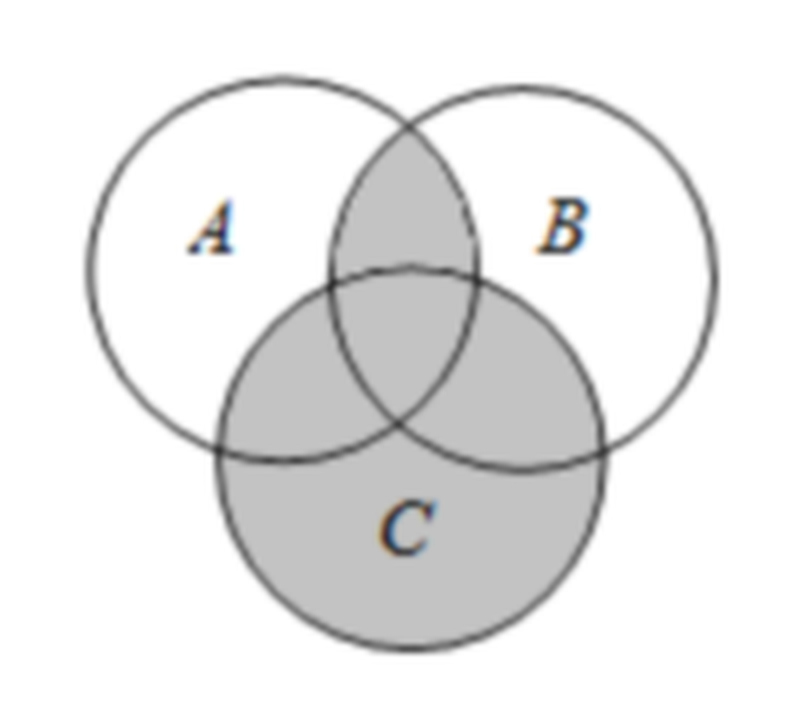
\includegraphics[width=0.30\textwidth]{figures/venn_ABcap_plus_C.png}
\end{center}

\keepwithprev
A. $(A\cup C)\cap(B\cup C)$\qquad B. $(A\cup B)\cap(A\cup C)$

C. $(A\cup B)\cap(B\cup C)$\qquad D. $(A\cup B)\cap C$

\ans{$A$}

\item 设 $f(x)=(x^2-6x+c_1)(x^2-6x+c_2)$，其中 $c_1\geqslant c_2$，集合

$M=\{x\mid f(x)=0\}=\{x_1,x_2,x_3\}\sub\Z$，则下列命题中不正确的是\mbox{（\quad）}

\keepwithprev
A. $3\in M$\qquad B. $c_2$ 可能为 $-16$

C. $c_1$ 可能为 $8$\qquad D. $M$ 中所有元素的和一定为 $9$

\ans{$C$}

\ifanswer
\solbegin
\step{若 $c_1$ 为 $8$，则 $c_2=9$，与 $c_1\geqslant c_2$ 矛盾，故选 $C$.}
\solend

\fi

\item 非空集合 $A$ 具有如下性质：①若 $x$、$y\in A$，则 $\dfrac{x}{y}\in A$；②若 $x$、$y\in A$，
则 $x+y\in A$；

由此可知：下列判断中，错误的是\mbox{（\quad）}

\keepwithprev
A. $-1\notin A$\qquad B. $\dfrac{2025}{2026}\in A$

C. 若 $x$、$y\in A$，则 $xy\in A$\qquad D. 若 $x$、$y\in A$，则 $x-y\in A$

\ans{$D$}

\ifanswer
\solbegin
\step{由题意得 $0\notin A$，$1\in A$，}
\step{对于 $A$，假设 $-1\in A$，则 $-1+1=0\in A$，矛盾，所以 $-1\notin A$，故 $A$ 正确；}
\step{对于 $B$，由 $1\in A$，得 $1+1=2\in A$，$2+1=3\in A$，$\cdots$，$2025\in A$，$2026\in A$，}
\step{所以 $\dfrac{2025}{2026}\in A$，故 $B$ 正确；}
\step{对于 $C$，因为 $1\in A$，$x\in A$，所以 $\dfrac1x\in A$，又因为 $y\in A$，
所以 $\dfrac{y}{\frac1x}=xy\in A$，}
\step{故 $C$ 正确；}
\step{对于 $D$，因为 $1\in A$，$2\in A$，若 $x=1$，$y=2$，则 $x-y=-1\notin A$，故 $D$ 错误.}
\step{故选 $D$.}
\solend

\fi

\end{enumerate}

\bigsec{三、解答题}

\begin{enumerate}
\setcounter{enumi}{13}

% 注：原卷本题题干把「$=0$」印在右花括号之外（$A=\{x\mid x^2-mx+4m-16\}=0$），
%     而其自己的【解析】印在括号之内（$A=\{x\mid x^2-mx+4m-16=0\}$）——原卷前后不一致，
%     本稿按解析与题目本意把 $=0$ 排在括号内，见文件头「排版差异」⑧。
\item 已知集合 $A=\{x\mid x^2-mx+4m-16=0\}$，$B=\{x\mid 1<x<4,x\in\N\}$，
$C=\{x\mid ax+2>0\}$，若 $A\cap B\neq\varnothing$，$A\cap C=\varnothing$，求实数 $m$ 的值以及
相应实数 $a$ 的取值范围.

\ifanswer
\solbegin
\step{集合 $A=\{x\mid x^2-mx+4m-16=0\}$，由 $\Delta=(-m)^2-4(4m-16)=(m-8)^2\geqslant0$，}
\step{所以当 $m=8$ 时，集合 $A=\{4\}$，当 $m\neq8$ 时，集合
$A=\left\{\dfrac{m-|m-8|}{2},\dfrac{m+|m-8|}{2}\right\}$，}
\step{集合 $B=\{x\mid 1<x<4,x\in\N\}$，得集合 $B=\{2,3\}$.}
\step{集合 $C=\{x\mid ax+2>0\}$，当 $a=0$ 时，集合 $C=\{x\mid x\in\R\}$，}
\step{当 $a<0$ 时，集合 $C=\left\{x\mid x<\dfrac2a\right\}$，当 $a>0$ 时，集合
$C=\left\{x\mid x>\dfrac2a\right\}$，}
\step{由 $A\cap B$ 非空得，$m=6$ 时，集合 $A=\{2,4\}$，$m=7$ 时，集合 $A=\{3,4\}$.}
\step{由 $A\cap C=\varnothing$，得 $m=6$ 或 $m=7$ 时，$a<0$ 或 $0<a<\dfrac12$ 符合要求.}
\solend

\fi

\ansspace[9]

\item 已知 $a>b>c$，$a+b+c=0$，方程 $ax^2+bx+c=0$ 的两个实根为 $x_1$、$x_2$.

\begin{enumerate}[label=(\arabic*)]
\item 证明：$-\dfrac12<\dfrac ba<1$；
% 注：此小问前加了 4pt 间距——不加时紧凑版该行的 $x_1^2$ 上标与下标恰好同箱，
%     pdftotext 抽正文会把上标当重影丢掉，make check 的正文指纹就对不上（纯抽取抖动，
%     版面与内容无差别，见 2026-09-20 入库注）。
\vspace{4pt}
\item 若 $x_1^2+x_1x_2+x_2^2=1$，求 $x_1^2-x_1x_2+x_2^2$.
\end{enumerate}

\ifanswer
\solbegin
\stepm{(1)}{因为 $a>b>c$，$a+b+c=0$，所以 $a>0$，$c<0$，$c=-a-b$，}
\step{由 $a>b$ 得 $\dfrac ba<1$ ①，由 $b>c$ 得 $b>-a-b$，即 $2b>-a$，即 $\dfrac ba>-\dfrac12$ ②，}
\step{由①②得 $-\dfrac12<\dfrac ba<1$；}
\stepm{(2)}{若 $x_1^2+x_1x_2+x_2^2=1$，则 $(x_1+x_2)^2-x_1x_2=1$，}
% 注：本行的连等式与原卷自己的结论对不上（照抄原卷、未改）——原卷印作
%     (b/a)²-b/a+1=1，则解出的应是 0 或 1；按 c=-a-b 应为 (b/a)²+b/a+1=1，
%     解得 0 或 -1（-1 因 c<0 舍去），恰与下一行「0 或 -1（舍去）」吻合。
%     详见文件头「原卷存疑」①。
\step{则 $\left(\dfrac ba\right)^2-\dfrac ca=\dfrac{b^2-ac}{a^2}
=\left(\dfrac ba\right)^2-\dfrac ba+1=1$，解得 $\dfrac ba=0$ 或 $-1$（舍去），}
\step{故 $\dfrac ba=0$，$\dfrac ca=-1$，}
\step{所以 $x_1^2-x_1x_2+x_2^2=(x_1+x_2)^2-3x_1x_2=\left(\dfrac ba\right)^2-3\times\dfrac ca=3$.}
\solend

\fi

\ansspace[6]

\item 已知方程 $x^2+px+q=0$ 与方程 $x^2+(p-3)x+2q+1=0$ 分别都有两个不相等的实根，若
他们的解集分别为 $A$、$B$，且 $A\cup B=\{1,2,5\}$，求 $p$、$q$、$A$、$B$.

\ifanswer
\solbegin
\step{两方程分别有两个不相等的实数根，而根的并集只有 $3$ 个元素，}
\step{则两方程有一公共根. 分类讨论：}
\stepm{（1）}{公共根为 $1$ 时，$x=1$ 分别代入两方程：}
\step{$\begin{cases}p+q+1=0\\ p-3+2q+1+1=0\end{cases}$，解得 $p=-3$，$q=2$，}
\step{两方程变为 $x^2-3x+2=0$，解得 $x=1$ 或 $x=2$，}
\step{$x^2-6x+5=0$ 解得 $x=1$ 或 $x=5$，满足题意.}
\stepm{（2）}{公共根为 $2$ 时，$x=2$ 分别代入两方程：}
\step{$\begin{cases}4+2p+q=0\\ 4+2p-6+2q+1=0\end{cases}$，解得 $p=-\dfrac92$，$q=5$，}
\step{第一个方程变为 $2x^2-9x+10=0$，解得 $x=2$ 或 $x=\dfrac52$，不满足题意，舍去.}
\stepm{（3）}{公共根为 $5$ 时，$x=5$ 分别代入两方程：}
\step{$\begin{cases}25+5p+q=0\\ 25+5p-15+2q+1=0\end{cases}$，解得 $p=-\dfrac{39}{5}$，$q=14$，}
\step{第一个方程变为 $5x^2-39x+70=0$，解得 $x=5$ 或 $x=\dfrac{14}{5}$，不满足题意，舍去.}
\step{综上，$p=-3$，$q=2$，$A=\{1,2\}$，$B=\{1,5\}$.}
\solend

\fi

\ansspace[8]

\item 对于集合 $A=\{a_1,a_2,\cdots,a_n\}(n\in\Z,n\geqslant3)$，其中每个元素均为正整数，如果
任意去掉其
中一个元素 $a_i(i=1,2,3\cdots,n)$ 之后，剩余的所有元素组成集合 $A_i(i=1,2,\cdots,n)$，并且
$A_i$ 都能分为两个集合 $B$ 和 $C$，满足 $B\cap C=\varnothing,B\cup C=A_i$，其中 $B$ 和 $C$
的所有元素之和相
等，就称集合 $A$ 为“可分集合”.

\begin{enumerate}[label=(\arabic*)]
\item 判断集合 $\{1,3,5,7,9,11,13\}$ 是否是“可分集合”（不必写过程）；
\item 用反证法证明：五个元素的集合 $A=\{a_1,a_2,a_3,a_4,a_5\}$ 一定不是“可分集合”；
\item 已知集合 $A=\{a_1,a_2,\cdots,a_n\}(n\in\Z,n\geqslant3)$ 是“可分集合”，求 $n$ 的最小值.
\end{enumerate}

\ifanswer
\solbegin
\stepm{(1)}{集合 $\{1,3,5,7,9,11,13\}$ 是“可分集合”；}
\stepm{(2)}{不妨设 $a_1<a_2<a_3<a_4<a_5$，}
\step{若去掉的元素为 $a_2$，将集合 $\{a_1,a_3,a_4,a_5\}$ 分成两个交集为空集的子集，}
\step{且两个子集元素之和相等，则有 $a_1+a_5=a_3+a_4$ ①，或者 $a_5=a_1+a_3+a_4$ ②；}
\step{若去掉的元素为 $a_1$，将集合 $\{a_2,a_3,a_4,a_5\}$ 分成两个交集为空集的子集，}
\step{且两个子集元素之和相等，则有 $a_2+a_5=a_3+a_4$ ③，或者 $a_5=a_2+a_3+a_4$ ④.}
\step{由①、③，得 $a_1=a_2$，矛盾；由①、④，得 $a_1=-a_2$，矛盾；}
\step{由②、③，得 $a_1=-a_2$，矛盾；由②、④，得 $a_1=a_2$ 矛盾.}
\step{因此当 $n=5$ 时，集合一定不是“可分集合”；}
\stepm{(3)}{①设集合 $A=\{a_1,a_2,\cdots,a_n\}$ 的所有元素之和为 $M$.}
\step{由题意得 $M-a_i(i=1,2,\cdots,n)$ 均为偶数，}
\step{因此 $a_i(i=1,2,\cdots,n)$ 均为奇数或偶数.}
\step{如果 $M$ 为奇数，则 $a_i(i=1,2,\cdots,n)$ 也均为奇数，}
\step{由于 $M=a_1+a_2+\cdots+a_n$，所以 $n$ 为奇数.}
\step{如果 $M$ 为偶数，则 $M-a_i(i=1,2,\cdots,n)$ 均为偶数，此时设 $a_i=2b_i$，}
\step{则 $\{b_1,b_2,\cdots,b_n\}$ 也是“可分集合”.}
\step{重复上述操作有限次，便可得各项均为奇数的“可分集合”，}
\step{此时各项之和也为奇数，则集合 $A$ 中元素个数 $n$ 为奇数.}
\step{综上所述，集合 $A$ 中元素个数为奇数.}
\step{②当 $n=3$ 时，显然任意集合 $\{a_1,a_2,a_3\}$ 不是“可分集合”.}
\step{当 $n=5$ 时，第（2）问已经证明不是“可分集合”.}
\step{当 $n=7$ 时，集合 $A=\{1,3,5,7,9,11,13\}$，}
\step{因为 $3+5+7+9=11+13$，$1+9+13=5+7+11$，$9+13=1+3+7+11$，}
\step{$1+3+5+11=7+13$，$1+9+11=3+5+13$，$3+7+9=1+5+13$，}
\step{$1+3+5+9=7+11$，则集合 $A$ 是“可分集合”，}
\step{所以集合 $A$ 中元素个数 $n$ 的最小值是 $7$.}
\solend

\fi

\ansspace*[10]

\end{enumerate}

\end{document}
"
%
% 原始材料是微信公众号图文（公众号「魔都数学加油站」连载「27学年高一 24」，2026-09-19 发布，
% 原文标题「27学年高一24——2026-2027年上海市复旦附中高一上周末作业3集合与逻辑、等式的性质」），
% 正文为 7 张 PNG 页（1080×1527，各页同尺寸）。原文本身就是一份**讲评版**——题目下方直接印出
% 【答案】或【解析】。试题文字、答案与解析均照原卷录入，未改内容。
% 卷面上的粉色斜水印「魔都数学加油站」属水印，未录入。
%
% 卷首标题：原卷印作「2026-2027 年复旦附中高一上周末作业 3」（公众号标题里有「上海市」三字，
% 卷面标题行没有，本稿照卷面），年份区间按全稿惯例排 en dash，前缀照原卷保留「年」。
%
% 与原卷的排版差异（均已在 README「说明」中交代）：
%   ① 原文自**第 3 题**起（第 1、2 题未在该文中发布），故本稿题号亦自 3 起；
%   ② 原卷本就印有「一、填空题」「二、选择题」「三、解答题」三节标题，本稿照原卷分节，
%      只把标题改排成全稿统一的「大节标题」样式；
%   ③ 原卷第 11 题的答案「A」直接印在题干末尾的括号内，第 12、13 题的括号空着、答案写在
%      解析末句「故选 C／D」里，本稿统一改为试卷版隐去、答案版以 \ans{} 给出（第 12、13 题
%      另附【解析】），使两版彻底分离；
%   ④ 原卷的集合／数集符号正体与粗体混用（第 8 题题干的 $\mathbf{R}$、第 9 题题干的
%      $\mathbf{N}$、第 12 题题干的 $\mathbf{Z}$ 为粗体，第 14 题解析的 $N$、$R$ 为斜体），
%      本稿按全稿惯例统一写作 $\R$、$\N$、$\Z$；
%   ⑤ 原卷填空的横线约两个字宽，本稿按全稿惯例统一排 \blankline[4.4em]；
%   ⑥ 第 11 题的 Venn 图原卷印在上一页末尾（第 10 题解析右侧、「二、选择题」标题旁），
%      本稿移至第 11 题题干之后；图取原卷截图、4× LANCZOS 放大
%      （figures/venn_ABcap_plus_C.png，阴影为 $A\cap B$ 的交与整个 $C$，即 $(A\cap B)\cup C$）；
%   ⑦ 原卷自印副标题「集合与逻辑、等式的性质」，本稿照录（与 高一14 同例，未改用惯例副标题）；
%   ⑧ 第 14 题题干原卷把「$=0$」印在右花括号**之外**（作
%      $A=\{x\mid x^2-mx+4m-16\}=0$），而它**自己的【解析】却印在括号之内**
%      （作 $A=\{x\mid x^2-mx+4m-16=0\}$）——原卷前后不一致；按原卷解析与题目本意，
%      本稿题干的 $=0$ 排在括号**之内**（与 高一b 第 13 题「原卷漏排 $A=$，本稿补上」同例）。
%
% 原卷存疑一处（已放大到能看清字形后核对，无法确证原意，本稿照抄原卷、未改）：
%   ① 第 15(2)【解析】的连等式印作
%      $\left(\frac ba\right)^2-\frac ca=\frac{b^2-ac}{a^2}=\left(\frac ba\right)^2-\frac ba+1=1$，
%      解得 $\frac ba=0$ 或 $-1$（舍去）——但由 $c=-a-b$ 应得 $\frac{b^2-ac}{a^2}
%      =\left(\frac ba\right)^2+\frac ba+1$（原卷把「$+\frac ba$」印成了「$-\frac ba$」）：
%      按原卷那行解出的是 $0$ 或 $1$，与其自己的结论「$0$ 或 $-1$」对不上；而按
%      $+\frac ba$ 解恰得 $0$ 或 $-1$（$-1$ 因 $c<0$ 舍去），与后文吻合。原卷显系笔误，
%      本稿照抄原卷（见源码中该处上方注释）。

\documentclass[a4paper,11pt]{article}
\usepackage{common}

\begin{document}

\examtitlest[3]{2026--2027 年复旦附中高一上周末作业 3}{集合与逻辑、等式的性质}

\bigsec{一、填空题}

\begin{enumerate}
\setcounter{enumi}{2}

\item 设 $M=\{x\mid y^2=x+2\}$，$N=\{x\mid y^2=-2x+8\}$，则 $M\cap N=$ \blankline[4.4em].

\ifanswer
\solbegin
\step{$M=[-2,+\infty)$，$N=(-\infty,4]$，则 $M\cap N=[-2,4]$.}
\solend

\fi

\item 若“$x\geqslant a$”是“$|x|\leqslant2$”的必要条件，则实数 $a$ 的取值集合是 \blankline[4.4em].

\ans{$(-\infty,-2]$}

\item 某校一年级的 $200$ 人中，爱好数学的有 $95$ 人，爱好体育的有 $156$ 人，则数学体育都爱好
的至少有 \blankline[4.4em] 人.

\ifanswer
\solbegin
\step{数学体育都爱好的至少有 $95+156-200=51$ 人.}
\solend

\fi

\item 已知 $x$ 为实数，且 $x^2+\dfrac{1}{x^2}=3$，则 $x^3+\dfrac{1}{x^3}$ 的值是 \blankline[4.4em].

\ifanswer
\solbegin
\step{因为 $x^2+\dfrac{1}{x^2}=\left(x+\dfrac1x\right)^2-2=3$，所以 $x+\dfrac1x=\pm\sqrt5$，}
\step{所以 $x^3+\dfrac{1}{x^3}=\left(x+\dfrac1x\right)\left(x^2-1+\dfrac{1}{x^2}\right)=\pm2\sqrt5$.}
\solend

\fi

\item 非空集合 $A=\{x\mid a+1\leqslant x<2a-1\}$，$B=\{x\mid-2\leqslant x\leqslant5\}$，
若 $A\sub(A\cap B)$，则 $a$ 的取值范围是 \blankline[4.4em].

\ifanswer
\solbegin
\step{当 $a+1<2a-1$，即 $a>2$ 时，$A\neq\varnothing$，由 $A\sub(A\cap B)$ 得 $A\sub B$，}
\step{得 $\begin{cases}a+1\geqslant-2\\ 2a-1\leqslant5\end{cases}$，解得 $-3\leqslant a\leqslant3$，所以 $2<a\leqslant3$.}
\solend

\fi

\item 已知集合 $\{x\mid(x-1)(x^2-x+a)=0,x\in\R\}$ 中的所有元素之和为 $1$，则实数 $a$ 的取值范
围是 \blankline[4.4em].

\ifanswer
\solbegin
\step{令 $x-1=0$，得 $x=1$，}
\stepm{①}{若 $x^2-x+a=0$ 无实数根，则 $\Delta=1-4a<0$，解得 $a>\dfrac14$，}
\step{此时集合只有元素 $1$，符合题意；}
\stepm{②}{若 $x^2-x+a=0$ 有两个相等的实数根，则 $\Delta=1-4a=0$，解得 $a=\dfrac14$，}
\step{此时方程为 $x^2-x+\dfrac14=0$，解得 $x=\dfrac12$，此时集合为 $\left\{1,\dfrac12\right\}$，不合题意；}
\stepm{③}{若 $x^2-x+a=0$ 有两个不相等的实数根，则 $\Delta=1-4a>0$，解得 $a<\dfrac14$，}
\step{设方程 $x^2-x+a=0$ 的两个实根分别为 $x_1,x_2$，则 $x_1+x_2=1$，}
\step{若 $x_1\neq1,x_2\neq1$，则集合为 $\{1,x_1,x_2\}$，不合题意，}
\step{若 $x_1=1$，则 $x_2=0$，此时集合为 $\{1,0\}$，符合题意，所以 $a=x_1x_2=0$，}
\step{综上所述，实数 $a$ 的取值范围是 $\{0\}\cup\left(\dfrac14,+\infty\right)$.}
\solend

\fi

\item 集合 $A=\{m\mid m=2k,k\in\N,1\leqslant k\leqslant50\}$，
$B=\{n\mid n=i+j,i<j,i\in A,j\in A\}$，则 $B$ 中元素的个数是 \blankline[4.4em].

\ifanswer
\solbegin
\step{$B$ 中最小元素是 $6$，最大元素是 $198$，则 $B$ 中元素的个数是 $\dfrac{198-6}{2}+1=97$.}
\solend

\fi

\item 关于 $(x,y,z)$ 的方程组
$\begin{cases}x^2+y^2+25z^2=6zx+8yz\\ 3x^2+2y^2+z^2=240\end{cases}$ 的解集为 \blankline[4.4em].

\ifanswer
\solbegin
\step{由上式得 $(x^2-6xz+9z^2)+(y^2-8yz+16z^2)=0$，}
\step{则 $(x-3z)^2+(y-4z)^2=0$，}
\step{所以 $(x,y,z)=(3t,4t,t)$，$t$ 为实数，代入下式中 $27\cdot t^2+32t^2+t^2=60t^2=240$，}
\step{则 $t^2=4$，$t=\pm2$，所以 $(x,y,z)=(6,8,2),(-6,-8,-2)$.}
\solend

\fi

\end{enumerate}

\bigsec{二、选择题}

\begin{enumerate}
\setcounter{enumi}{10}

\item 下列表示图形中的阴影部分的是\mbox{（\quad）}

\begin{center}
% 图取原卷截图、4× LANCZOS 放大（原卷把图印在上一页末尾，本稿移至此处，见文件头⑥）。
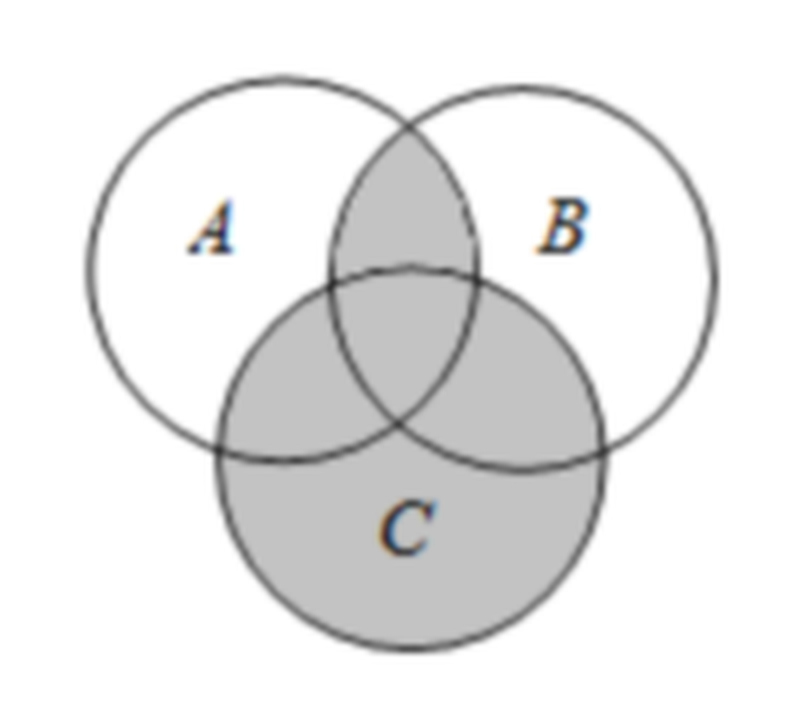
\includegraphics[width=0.30\textwidth]{figures/venn_ABcap_plus_C.png}
\end{center}

\keepwithprev
A. $(A\cup C)\cap(B\cup C)$\qquad B. $(A\cup B)\cap(A\cup C)$

C. $(A\cup B)\cap(B\cup C)$\qquad D. $(A\cup B)\cap C$

\ans{$A$}

\item 设 $f(x)=(x^2-6x+c_1)(x^2-6x+c_2)$，其中 $c_1\geqslant c_2$，集合

$M=\{x\mid f(x)=0\}=\{x_1,x_2,x_3\}\sub\Z$，则下列命题中不正确的是\mbox{（\quad）}

\keepwithprev
A. $3\in M$\qquad B. $c_2$ 可能为 $-16$

C. $c_1$ 可能为 $8$\qquad D. $M$ 中所有元素的和一定为 $9$

\ans{$C$}

\ifanswer
\solbegin
\step{若 $c_1$ 为 $8$，则 $c_2=9$，与 $c_1\geqslant c_2$ 矛盾，故选 $C$.}
\solend

\fi

\item 非空集合 $A$ 具有如下性质：①若 $x$、$y\in A$，则 $\dfrac{x}{y}\in A$；②若 $x$、$y\in A$，
则 $x+y\in A$；

由此可知：下列判断中，错误的是\mbox{（\quad）}

\keepwithprev
A. $-1\notin A$\qquad B. $\dfrac{2025}{2026}\in A$

C. 若 $x$、$y\in A$，则 $xy\in A$\qquad D. 若 $x$、$y\in A$，则 $x-y\in A$

\ans{$D$}

\ifanswer
\solbegin
\step{由题意得 $0\notin A$，$1\in A$，}
\step{对于 $A$，假设 $-1\in A$，则 $-1+1=0\in A$，矛盾，所以 $-1\notin A$，故 $A$ 正确；}
\step{对于 $B$，由 $1\in A$，得 $1+1=2\in A$，$2+1=3\in A$，$\cdots$，$2025\in A$，$2026\in A$，}
\step{所以 $\dfrac{2025}{2026}\in A$，故 $B$ 正确；}
\step{对于 $C$，因为 $1\in A$，$x\in A$，所以 $\dfrac1x\in A$，又因为 $y\in A$，
所以 $\dfrac{y}{\frac1x}=xy\in A$，}
\step{故 $C$ 正确；}
\step{对于 $D$，因为 $1\in A$，$2\in A$，若 $x=1$，$y=2$，则 $x-y=-1\notin A$，故 $D$ 错误.}
\step{故选 $D$.}
\solend

\fi

\end{enumerate}

\bigsec{三、解答题}

\begin{enumerate}
\setcounter{enumi}{13}

% 注：原卷本题题干把「$=0$」印在右花括号之外（$A=\{x\mid x^2-mx+4m-16\}=0$），
%     而其自己的【解析】印在括号之内（$A=\{x\mid x^2-mx+4m-16=0\}$）——原卷前后不一致，
%     本稿按解析与题目本意把 $=0$ 排在括号内，见文件头「排版差异」⑧。
\item 已知集合 $A=\{x\mid x^2-mx+4m-16=0\}$，$B=\{x\mid 1<x<4,x\in\N\}$，
$C=\{x\mid ax+2>0\}$，若 $A\cap B\neq\varnothing$，$A\cap C=\varnothing$，求实数 $m$ 的值以及
相应实数 $a$ 的取值范围.

\ifanswer
\solbegin
\step{集合 $A=\{x\mid x^2-mx+4m-16=0\}$，由 $\Delta=(-m)^2-4(4m-16)=(m-8)^2\geqslant0$，}
\step{所以当 $m=8$ 时，集合 $A=\{4\}$，当 $m\neq8$ 时，集合
$A=\left\{\dfrac{m-|m-8|}{2},\dfrac{m+|m-8|}{2}\right\}$，}
\step{集合 $B=\{x\mid 1<x<4,x\in\N\}$，得集合 $B=\{2,3\}$.}
\step{集合 $C=\{x\mid ax+2>0\}$，当 $a=0$ 时，集合 $C=\{x\mid x\in\R\}$，}
\step{当 $a<0$ 时，集合 $C=\left\{x\mid x<\dfrac2a\right\}$，当 $a>0$ 时，集合
$C=\left\{x\mid x>\dfrac2a\right\}$，}
\step{由 $A\cap B$ 非空得，$m=6$ 时，集合 $A=\{2,4\}$，$m=7$ 时，集合 $A=\{3,4\}$.}
\step{由 $A\cap C=\varnothing$，得 $m=6$ 或 $m=7$ 时，$a<0$ 或 $0<a<\dfrac12$ 符合要求.}
\solend

\fi

\ansspace[9]

\item 已知 $a>b>c$，$a+b+c=0$，方程 $ax^2+bx+c=0$ 的两个实根为 $x_1$、$x_2$.

\begin{enumerate}[label=(\arabic*)]
\item 证明：$-\dfrac12<\dfrac ba<1$；
% 注：此小问前加了 4pt 间距——不加时紧凑版该行的 $x_1^2$ 上标与下标恰好同箱，
%     pdftotext 抽正文会把上标当重影丢掉，make check 的正文指纹就对不上（纯抽取抖动，
%     版面与内容无差别，见 2026-09-20 入库注）。
\vspace{4pt}
\item 若 $x_1^2+x_1x_2+x_2^2=1$，求 $x_1^2-x_1x_2+x_2^2$.
\end{enumerate}

\ifanswer
\solbegin
\stepm{(1)}{因为 $a>b>c$，$a+b+c=0$，所以 $a>0$，$c<0$，$c=-a-b$，}
\step{由 $a>b$ 得 $\dfrac ba<1$ ①，由 $b>c$ 得 $b>-a-b$，即 $2b>-a$，即 $\dfrac ba>-\dfrac12$ ②，}
\step{由①②得 $-\dfrac12<\dfrac ba<1$；}
\stepm{(2)}{若 $x_1^2+x_1x_2+x_2^2=1$，则 $(x_1+x_2)^2-x_1x_2=1$，}
% 注：本行的连等式与原卷自己的结论对不上（照抄原卷、未改）——原卷印作
%     (b/a)²-b/a+1=1，则解出的应是 0 或 1；按 c=-a-b 应为 (b/a)²+b/a+1=1，
%     解得 0 或 -1（-1 因 c<0 舍去），恰与下一行「0 或 -1（舍去）」吻合。
%     详见文件头「原卷存疑」①。
\step{则 $\left(\dfrac ba\right)^2-\dfrac ca=\dfrac{b^2-ac}{a^2}
=\left(\dfrac ba\right)^2-\dfrac ba+1=1$，解得 $\dfrac ba=0$ 或 $-1$（舍去），}
\step{故 $\dfrac ba=0$，$\dfrac ca=-1$，}
\step{所以 $x_1^2-x_1x_2+x_2^2=(x_1+x_2)^2-3x_1x_2=\left(\dfrac ba\right)^2-3\times\dfrac ca=3$.}
\solend

\fi

\ansspace[6]

\item 已知方程 $x^2+px+q=0$ 与方程 $x^2+(p-3)x+2q+1=0$ 分别都有两个不相等的实根，若
他们的解集分别为 $A$、$B$，且 $A\cup B=\{1,2,5\}$，求 $p$、$q$、$A$、$B$.

\ifanswer
\solbegin
\step{两方程分别有两个不相等的实数根，而根的并集只有 $3$ 个元素，}
\step{则两方程有一公共根. 分类讨论：}
\stepm{（1）}{公共根为 $1$ 时，$x=1$ 分别代入两方程：}
\step{$\begin{cases}p+q+1=0\\ p-3+2q+1+1=0\end{cases}$，解得 $p=-3$，$q=2$，}
\step{两方程变为 $x^2-3x+2=0$，解得 $x=1$ 或 $x=2$，}
\step{$x^2-6x+5=0$ 解得 $x=1$ 或 $x=5$，满足题意.}
\stepm{（2）}{公共根为 $2$ 时，$x=2$ 分别代入两方程：}
\step{$\begin{cases}4+2p+q=0\\ 4+2p-6+2q+1=0\end{cases}$，解得 $p=-\dfrac92$，$q=5$，}
\step{第一个方程变为 $2x^2-9x+10=0$，解得 $x=2$ 或 $x=\dfrac52$，不满足题意，舍去.}
\stepm{（3）}{公共根为 $5$ 时，$x=5$ 分别代入两方程：}
\step{$\begin{cases}25+5p+q=0\\ 25+5p-15+2q+1=0\end{cases}$，解得 $p=-\dfrac{39}{5}$，$q=14$，}
\step{第一个方程变为 $5x^2-39x+70=0$，解得 $x=5$ 或 $x=\dfrac{14}{5}$，不满足题意，舍去.}
\step{综上，$p=-3$，$q=2$，$A=\{1,2\}$，$B=\{1,5\}$.}
\solend

\fi

\ansspace[8]

\item 对于集合 $A=\{a_1,a_2,\cdots,a_n\}(n\in\Z,n\geqslant3)$，其中每个元素均为正整数，如果
任意去掉其
中一个元素 $a_i(i=1,2,3\cdots,n)$ 之后，剩余的所有元素组成集合 $A_i(i=1,2,\cdots,n)$，并且
$A_i$ 都能分为两个集合 $B$ 和 $C$，满足 $B\cap C=\varnothing,B\cup C=A_i$，其中 $B$ 和 $C$
的所有元素之和相
等，就称集合 $A$ 为“可分集合”.

\begin{enumerate}[label=(\arabic*)]
\item 判断集合 $\{1,3,5,7,9,11,13\}$ 是否是“可分集合”（不必写过程）；
\item 用反证法证明：五个元素的集合 $A=\{a_1,a_2,a_3,a_4,a_5\}$ 一定不是“可分集合”；
\item 已知集合 $A=\{a_1,a_2,\cdots,a_n\}(n\in\Z,n\geqslant3)$ 是“可分集合”，求 $n$ 的最小值.
\end{enumerate}

\ifanswer
\solbegin
\stepm{(1)}{集合 $\{1,3,5,7,9,11,13\}$ 是“可分集合”；}
\stepm{(2)}{不妨设 $a_1<a_2<a_3<a_4<a_5$，}
\step{若去掉的元素为 $a_2$，将集合 $\{a_1,a_3,a_4,a_5\}$ 分成两个交集为空集的子集，}
\step{且两个子集元素之和相等，则有 $a_1+a_5=a_3+a_4$ ①，或者 $a_5=a_1+a_3+a_4$ ②；}
\step{若去掉的元素为 $a_1$，将集合 $\{a_2,a_3,a_4,a_5\}$ 分成两个交集为空集的子集，}
\step{且两个子集元素之和相等，则有 $a_2+a_5=a_3+a_4$ ③，或者 $a_5=a_2+a_3+a_4$ ④.}
\step{由①、③，得 $a_1=a_2$，矛盾；由①、④，得 $a_1=-a_2$，矛盾；}
\step{由②、③，得 $a_1=-a_2$，矛盾；由②、④，得 $a_1=a_2$ 矛盾.}
\step{因此当 $n=5$ 时，集合一定不是“可分集合”；}
\stepm{(3)}{①设集合 $A=\{a_1,a_2,\cdots,a_n\}$ 的所有元素之和为 $M$.}
\step{由题意得 $M-a_i(i=1,2,\cdots,n)$ 均为偶数，}
\step{因此 $a_i(i=1,2,\cdots,n)$ 均为奇数或偶数.}
\step{如果 $M$ 为奇数，则 $a_i(i=1,2,\cdots,n)$ 也均为奇数，}
\step{由于 $M=a_1+a_2+\cdots+a_n$，所以 $n$ 为奇数.}
\step{如果 $M$ 为偶数，则 $M-a_i(i=1,2,\cdots,n)$ 均为偶数，此时设 $a_i=2b_i$，}
\step{则 $\{b_1,b_2,\cdots,b_n\}$ 也是“可分集合”.}
\step{重复上述操作有限次，便可得各项均为奇数的“可分集合”，}
\step{此时各项之和也为奇数，则集合 $A$ 中元素个数 $n$ 为奇数.}
\step{综上所述，集合 $A$ 中元素个数为奇数.}
\step{②当 $n=3$ 时，显然任意集合 $\{a_1,a_2,a_3\}$ 不是“可分集合”.}
\step{当 $n=5$ 时，第（2）问已经证明不是“可分集合”.}
\step{当 $n=7$ 时，集合 $A=\{1,3,5,7,9,11,13\}$，}
\step{因为 $3+5+7+9=11+13$，$1+9+13=5+7+11$，$9+13=1+3+7+11$，}
\step{$1+3+5+11=7+13$，$1+9+11=3+5+13$，$3+7+9=1+5+13$，}
\step{$1+3+5+9=7+11$，则集合 $A$ 是“可分集合”，}
\step{所以集合 $A$ 中元素个数 $n$ 的最小值是 $7$.}
\solend

\fi

\ansspace*[10]

\end{enumerate}

\end{document}
"
% 紧凑版：xelatex "\def\iscompact{1}% 高一24_复旦附中_周末作业3.tex
%   —— 高一上数学「2026-2027 年复旦附中高一上周末作业 3」（试卷版/答案版）
% 试卷版：xelatex 高一24_复旦附中_周末作业3.tex
% 答案版：xelatex "\def\isanswer{1}% 高一24_复旦附中_周末作业3.tex
%   —— 高一上数学「2026-2027 年复旦附中高一上周末作业 3」（试卷版/答案版）
% 试卷版：xelatex 高一24_复旦附中_周末作业3.tex
% 答案版：xelatex "\def\isanswer{1}\input{高一24_复旦附中_周末作业3.tex}"
% 紧凑版：xelatex "\def\iscompact{1}\input{高一24_复旦附中_周末作业3.tex}"
%
% 原始材料是微信公众号图文（公众号「魔都数学加油站」连载「27学年高一 24」，2026-09-19 发布，
% 原文标题「27学年高一24——2026-2027年上海市复旦附中高一上周末作业3集合与逻辑、等式的性质」），
% 正文为 7 张 PNG 页（1080×1527，各页同尺寸）。原文本身就是一份**讲评版**——题目下方直接印出
% 【答案】或【解析】。试题文字、答案与解析均照原卷录入，未改内容。
% 卷面上的粉色斜水印「魔都数学加油站」属水印，未录入。
%
% 卷首标题：原卷印作「2026-2027 年复旦附中高一上周末作业 3」（公众号标题里有「上海市」三字，
% 卷面标题行没有，本稿照卷面），年份区间按全稿惯例排 en dash，前缀照原卷保留「年」。
%
% 与原卷的排版差异（均已在 README「说明」中交代）：
%   ① 原文自**第 3 题**起（第 1、2 题未在该文中发布），故本稿题号亦自 3 起；
%   ② 原卷本就印有「一、填空题」「二、选择题」「三、解答题」三节标题，本稿照原卷分节，
%      只把标题改排成全稿统一的「大节标题」样式；
%   ③ 原卷第 11 题的答案「A」直接印在题干末尾的括号内，第 12、13 题的括号空着、答案写在
%      解析末句「故选 C／D」里，本稿统一改为试卷版隐去、答案版以 \ans{} 给出（第 12、13 题
%      另附【解析】），使两版彻底分离；
%   ④ 原卷的集合／数集符号正体与粗体混用（第 8 题题干的 $\mathbf{R}$、第 9 题题干的
%      $\mathbf{N}$、第 12 题题干的 $\mathbf{Z}$ 为粗体，第 14 题解析的 $N$、$R$ 为斜体），
%      本稿按全稿惯例统一写作 $\R$、$\N$、$\Z$；
%   ⑤ 原卷填空的横线约两个字宽，本稿按全稿惯例统一排 \blankline[4.4em]；
%   ⑥ 第 11 题的 Venn 图原卷印在上一页末尾（第 10 题解析右侧、「二、选择题」标题旁），
%      本稿移至第 11 题题干之后；图取原卷截图、4× LANCZOS 放大
%      （figures/venn_ABcap_plus_C.png，阴影为 $A\cap B$ 的交与整个 $C$，即 $(A\cap B)\cup C$）；
%   ⑦ 原卷自印副标题「集合与逻辑、等式的性质」，本稿照录（与 高一14 同例，未改用惯例副标题）；
%   ⑧ 第 14 题题干原卷把「$=0$」印在右花括号**之外**（作
%      $A=\{x\mid x^2-mx+4m-16\}=0$），而它**自己的【解析】却印在括号之内**
%      （作 $A=\{x\mid x^2-mx+4m-16=0\}$）——原卷前后不一致；按原卷解析与题目本意，
%      本稿题干的 $=0$ 排在括号**之内**（与 高一b 第 13 题「原卷漏排 $A=$，本稿补上」同例）。
%
% 原卷存疑一处（已放大到能看清字形后核对，无法确证原意，本稿照抄原卷、未改）：
%   ① 第 15(2)【解析】的连等式印作
%      $\left(\frac ba\right)^2-\frac ca=\frac{b^2-ac}{a^2}=\left(\frac ba\right)^2-\frac ba+1=1$，
%      解得 $\frac ba=0$ 或 $-1$（舍去）——但由 $c=-a-b$ 应得 $\frac{b^2-ac}{a^2}
%      =\left(\frac ba\right)^2+\frac ba+1$（原卷把「$+\frac ba$」印成了「$-\frac ba$」）：
%      按原卷那行解出的是 $0$ 或 $1$，与其自己的结论「$0$ 或 $-1$」对不上；而按
%      $+\frac ba$ 解恰得 $0$ 或 $-1$（$-1$ 因 $c<0$ 舍去），与后文吻合。原卷显系笔误，
%      本稿照抄原卷（见源码中该处上方注释）。

\documentclass[a4paper,11pt]{article}
\usepackage{common}

\begin{document}

\examtitlest[3]{2026--2027 年复旦附中高一上周末作业 3}{集合与逻辑、等式的性质}

\bigsec{一、填空题}

\begin{enumerate}
\setcounter{enumi}{2}

\item 设 $M=\{x\mid y^2=x+2\}$，$N=\{x\mid y^2=-2x+8\}$，则 $M\cap N=$ \blankline[4.4em].

\ifanswer
\solbegin
\step{$M=[-2,+\infty)$，$N=(-\infty,4]$，则 $M\cap N=[-2,4]$.}
\solend

\fi

\item 若“$x\geqslant a$”是“$|x|\leqslant2$”的必要条件，则实数 $a$ 的取值集合是 \blankline[4.4em].

\ans{$(-\infty,-2]$}

\item 某校一年级的 $200$ 人中，爱好数学的有 $95$ 人，爱好体育的有 $156$ 人，则数学体育都爱好
的至少有 \blankline[4.4em] 人.

\ifanswer
\solbegin
\step{数学体育都爱好的至少有 $95+156-200=51$ 人.}
\solend

\fi

\item 已知 $x$ 为实数，且 $x^2+\dfrac{1}{x^2}=3$，则 $x^3+\dfrac{1}{x^3}$ 的值是 \blankline[4.4em].

\ifanswer
\solbegin
\step{因为 $x^2+\dfrac{1}{x^2}=\left(x+\dfrac1x\right)^2-2=3$，所以 $x+\dfrac1x=\pm\sqrt5$，}
\step{所以 $x^3+\dfrac{1}{x^3}=\left(x+\dfrac1x\right)\left(x^2-1+\dfrac{1}{x^2}\right)=\pm2\sqrt5$.}
\solend

\fi

\item 非空集合 $A=\{x\mid a+1\leqslant x<2a-1\}$，$B=\{x\mid-2\leqslant x\leqslant5\}$，
若 $A\sub(A\cap B)$，则 $a$ 的取值范围是 \blankline[4.4em].

\ifanswer
\solbegin
\step{当 $a+1<2a-1$，即 $a>2$ 时，$A\neq\varnothing$，由 $A\sub(A\cap B)$ 得 $A\sub B$，}
\step{得 $\begin{cases}a+1\geqslant-2\\ 2a-1\leqslant5\end{cases}$，解得 $-3\leqslant a\leqslant3$，所以 $2<a\leqslant3$.}
\solend

\fi

\item 已知集合 $\{x\mid(x-1)(x^2-x+a)=0,x\in\R\}$ 中的所有元素之和为 $1$，则实数 $a$ 的取值范
围是 \blankline[4.4em].

\ifanswer
\solbegin
\step{令 $x-1=0$，得 $x=1$，}
\stepm{①}{若 $x^2-x+a=0$ 无实数根，则 $\Delta=1-4a<0$，解得 $a>\dfrac14$，}
\step{此时集合只有元素 $1$，符合题意；}
\stepm{②}{若 $x^2-x+a=0$ 有两个相等的实数根，则 $\Delta=1-4a=0$，解得 $a=\dfrac14$，}
\step{此时方程为 $x^2-x+\dfrac14=0$，解得 $x=\dfrac12$，此时集合为 $\left\{1,\dfrac12\right\}$，不合题意；}
\stepm{③}{若 $x^2-x+a=0$ 有两个不相等的实数根，则 $\Delta=1-4a>0$，解得 $a<\dfrac14$，}
\step{设方程 $x^2-x+a=0$ 的两个实根分别为 $x_1,x_2$，则 $x_1+x_2=1$，}
\step{若 $x_1\neq1,x_2\neq1$，则集合为 $\{1,x_1,x_2\}$，不合题意，}
\step{若 $x_1=1$，则 $x_2=0$，此时集合为 $\{1,0\}$，符合题意，所以 $a=x_1x_2=0$，}
\step{综上所述，实数 $a$ 的取值范围是 $\{0\}\cup\left(\dfrac14,+\infty\right)$.}
\solend

\fi

\item 集合 $A=\{m\mid m=2k,k\in\N,1\leqslant k\leqslant50\}$，
$B=\{n\mid n=i+j,i<j,i\in A,j\in A\}$，则 $B$ 中元素的个数是 \blankline[4.4em].

\ifanswer
\solbegin
\step{$B$ 中最小元素是 $6$，最大元素是 $198$，则 $B$ 中元素的个数是 $\dfrac{198-6}{2}+1=97$.}
\solend

\fi

\item 关于 $(x,y,z)$ 的方程组
$\begin{cases}x^2+y^2+25z^2=6zx+8yz\\ 3x^2+2y^2+z^2=240\end{cases}$ 的解集为 \blankline[4.4em].

\ifanswer
\solbegin
\step{由上式得 $(x^2-6xz+9z^2)+(y^2-8yz+16z^2)=0$，}
\step{则 $(x-3z)^2+(y-4z)^2=0$，}
\step{所以 $(x,y,z)=(3t,4t,t)$，$t$ 为实数，代入下式中 $27\cdot t^2+32t^2+t^2=60t^2=240$，}
\step{则 $t^2=4$，$t=\pm2$，所以 $(x,y,z)=(6,8,2),(-6,-8,-2)$.}
\solend

\fi

\end{enumerate}

\bigsec{二、选择题}

\begin{enumerate}
\setcounter{enumi}{10}

\item 下列表示图形中的阴影部分的是\mbox{（\quad）}

\begin{center}
% 图取原卷截图、4× LANCZOS 放大（原卷把图印在上一页末尾，本稿移至此处，见文件头⑥）。
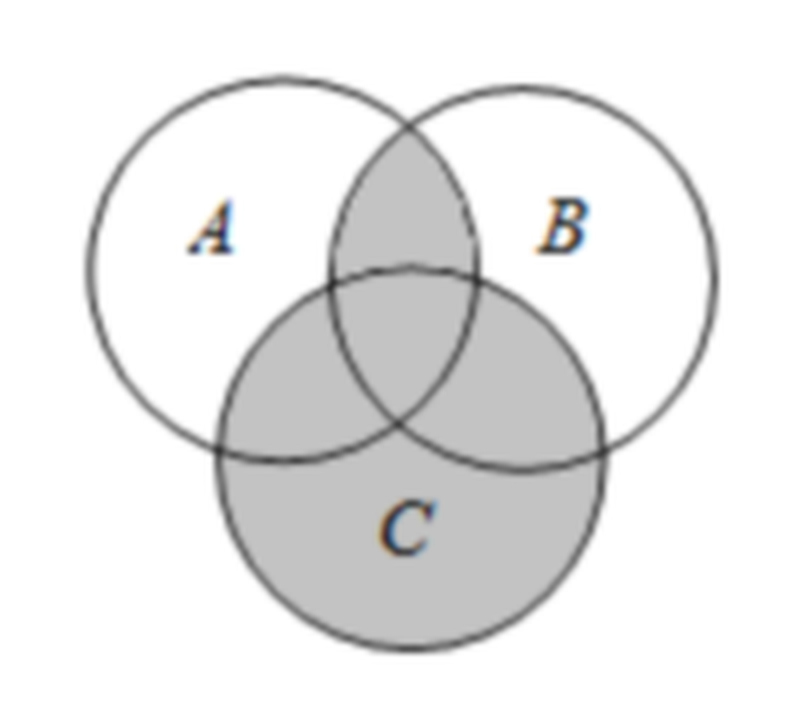
\includegraphics[width=0.30\textwidth]{figures/venn_ABcap_plus_C.png}
\end{center}

\keepwithprev
A. $(A\cup C)\cap(B\cup C)$\qquad B. $(A\cup B)\cap(A\cup C)$

C. $(A\cup B)\cap(B\cup C)$\qquad D. $(A\cup B)\cap C$

\ans{$A$}

\item 设 $f(x)=(x^2-6x+c_1)(x^2-6x+c_2)$，其中 $c_1\geqslant c_2$，集合

$M=\{x\mid f(x)=0\}=\{x_1,x_2,x_3\}\sub\Z$，则下列命题中不正确的是\mbox{（\quad）}

\keepwithprev
A. $3\in M$\qquad B. $c_2$ 可能为 $-16$

C. $c_1$ 可能为 $8$\qquad D. $M$ 中所有元素的和一定为 $9$

\ans{$C$}

\ifanswer
\solbegin
\step{若 $c_1$ 为 $8$，则 $c_2=9$，与 $c_1\geqslant c_2$ 矛盾，故选 $C$.}
\solend

\fi

\item 非空集合 $A$ 具有如下性质：①若 $x$、$y\in A$，则 $\dfrac{x}{y}\in A$；②若 $x$、$y\in A$，
则 $x+y\in A$；

由此可知：下列判断中，错误的是\mbox{（\quad）}

\keepwithprev
A. $-1\notin A$\qquad B. $\dfrac{2025}{2026}\in A$

C. 若 $x$、$y\in A$，则 $xy\in A$\qquad D. 若 $x$、$y\in A$，则 $x-y\in A$

\ans{$D$}

\ifanswer
\solbegin
\step{由题意得 $0\notin A$，$1\in A$，}
\step{对于 $A$，假设 $-1\in A$，则 $-1+1=0\in A$，矛盾，所以 $-1\notin A$，故 $A$ 正确；}
\step{对于 $B$，由 $1\in A$，得 $1+1=2\in A$，$2+1=3\in A$，$\cdots$，$2025\in A$，$2026\in A$，}
\step{所以 $\dfrac{2025}{2026}\in A$，故 $B$ 正确；}
\step{对于 $C$，因为 $1\in A$，$x\in A$，所以 $\dfrac1x\in A$，又因为 $y\in A$，
所以 $\dfrac{y}{\frac1x}=xy\in A$，}
\step{故 $C$ 正确；}
\step{对于 $D$，因为 $1\in A$，$2\in A$，若 $x=1$，$y=2$，则 $x-y=-1\notin A$，故 $D$ 错误.}
\step{故选 $D$.}
\solend

\fi

\end{enumerate}

\bigsec{三、解答题}

\begin{enumerate}
\setcounter{enumi}{13}

% 注：原卷本题题干把「$=0$」印在右花括号之外（$A=\{x\mid x^2-mx+4m-16\}=0$），
%     而其自己的【解析】印在括号之内（$A=\{x\mid x^2-mx+4m-16=0\}$）——原卷前后不一致，
%     本稿按解析与题目本意把 $=0$ 排在括号内，见文件头「排版差异」⑧。
\item 已知集合 $A=\{x\mid x^2-mx+4m-16=0\}$，$B=\{x\mid 1<x<4,x\in\N\}$，
$C=\{x\mid ax+2>0\}$，若 $A\cap B\neq\varnothing$，$A\cap C=\varnothing$，求实数 $m$ 的值以及
相应实数 $a$ 的取值范围.

\ifanswer
\solbegin
\step{集合 $A=\{x\mid x^2-mx+4m-16=0\}$，由 $\Delta=(-m)^2-4(4m-16)=(m-8)^2\geqslant0$，}
\step{所以当 $m=8$ 时，集合 $A=\{4\}$，当 $m\neq8$ 时，集合
$A=\left\{\dfrac{m-|m-8|}{2},\dfrac{m+|m-8|}{2}\right\}$，}
\step{集合 $B=\{x\mid 1<x<4,x\in\N\}$，得集合 $B=\{2,3\}$.}
\step{集合 $C=\{x\mid ax+2>0\}$，当 $a=0$ 时，集合 $C=\{x\mid x\in\R\}$，}
\step{当 $a<0$ 时，集合 $C=\left\{x\mid x<\dfrac2a\right\}$，当 $a>0$ 时，集合
$C=\left\{x\mid x>\dfrac2a\right\}$，}
\step{由 $A\cap B$ 非空得，$m=6$ 时，集合 $A=\{2,4\}$，$m=7$ 时，集合 $A=\{3,4\}$.}
\step{由 $A\cap C=\varnothing$，得 $m=6$ 或 $m=7$ 时，$a<0$ 或 $0<a<\dfrac12$ 符合要求.}
\solend

\fi

\ansspace[9]

\item 已知 $a>b>c$，$a+b+c=0$，方程 $ax^2+bx+c=0$ 的两个实根为 $x_1$、$x_2$.

\begin{enumerate}[label=(\arabic*)]
\item 证明：$-\dfrac12<\dfrac ba<1$；
% 注：此小问前加了 4pt 间距——不加时紧凑版该行的 $x_1^2$ 上标与下标恰好同箱，
%     pdftotext 抽正文会把上标当重影丢掉，make check 的正文指纹就对不上（纯抽取抖动，
%     版面与内容无差别，见 2026-09-20 入库注）。
\vspace{4pt}
\item 若 $x_1^2+x_1x_2+x_2^2=1$，求 $x_1^2-x_1x_2+x_2^2$.
\end{enumerate}

\ifanswer
\solbegin
\stepm{(1)}{因为 $a>b>c$，$a+b+c=0$，所以 $a>0$，$c<0$，$c=-a-b$，}
\step{由 $a>b$ 得 $\dfrac ba<1$ ①，由 $b>c$ 得 $b>-a-b$，即 $2b>-a$，即 $\dfrac ba>-\dfrac12$ ②，}
\step{由①②得 $-\dfrac12<\dfrac ba<1$；}
\stepm{(2)}{若 $x_1^2+x_1x_2+x_2^2=1$，则 $(x_1+x_2)^2-x_1x_2=1$，}
% 注：本行的连等式与原卷自己的结论对不上（照抄原卷、未改）——原卷印作
%     (b/a)²-b/a+1=1，则解出的应是 0 或 1；按 c=-a-b 应为 (b/a)²+b/a+1=1，
%     解得 0 或 -1（-1 因 c<0 舍去），恰与下一行「0 或 -1（舍去）」吻合。
%     详见文件头「原卷存疑」①。
\step{则 $\left(\dfrac ba\right)^2-\dfrac ca=\dfrac{b^2-ac}{a^2}
=\left(\dfrac ba\right)^2-\dfrac ba+1=1$，解得 $\dfrac ba=0$ 或 $-1$（舍去），}
\step{故 $\dfrac ba=0$，$\dfrac ca=-1$，}
\step{所以 $x_1^2-x_1x_2+x_2^2=(x_1+x_2)^2-3x_1x_2=\left(\dfrac ba\right)^2-3\times\dfrac ca=3$.}
\solend

\fi

\ansspace[6]

\item 已知方程 $x^2+px+q=0$ 与方程 $x^2+(p-3)x+2q+1=0$ 分别都有两个不相等的实根，若
他们的解集分别为 $A$、$B$，且 $A\cup B=\{1,2,5\}$，求 $p$、$q$、$A$、$B$.

\ifanswer
\solbegin
\step{两方程分别有两个不相等的实数根，而根的并集只有 $3$ 个元素，}
\step{则两方程有一公共根. 分类讨论：}
\stepm{（1）}{公共根为 $1$ 时，$x=1$ 分别代入两方程：}
\step{$\begin{cases}p+q+1=0\\ p-3+2q+1+1=0\end{cases}$，解得 $p=-3$，$q=2$，}
\step{两方程变为 $x^2-3x+2=0$，解得 $x=1$ 或 $x=2$，}
\step{$x^2-6x+5=0$ 解得 $x=1$ 或 $x=5$，满足题意.}
\stepm{（2）}{公共根为 $2$ 时，$x=2$ 分别代入两方程：}
\step{$\begin{cases}4+2p+q=0\\ 4+2p-6+2q+1=0\end{cases}$，解得 $p=-\dfrac92$，$q=5$，}
\step{第一个方程变为 $2x^2-9x+10=0$，解得 $x=2$ 或 $x=\dfrac52$，不满足题意，舍去.}
\stepm{（3）}{公共根为 $5$ 时，$x=5$ 分别代入两方程：}
\step{$\begin{cases}25+5p+q=0\\ 25+5p-15+2q+1=0\end{cases}$，解得 $p=-\dfrac{39}{5}$，$q=14$，}
\step{第一个方程变为 $5x^2-39x+70=0$，解得 $x=5$ 或 $x=\dfrac{14}{5}$，不满足题意，舍去.}
\step{综上，$p=-3$，$q=2$，$A=\{1,2\}$，$B=\{1,5\}$.}
\solend

\fi

\ansspace[8]

\item 对于集合 $A=\{a_1,a_2,\cdots,a_n\}(n\in\Z,n\geqslant3)$，其中每个元素均为正整数，如果
任意去掉其
中一个元素 $a_i(i=1,2,3\cdots,n)$ 之后，剩余的所有元素组成集合 $A_i(i=1,2,\cdots,n)$，并且
$A_i$ 都能分为两个集合 $B$ 和 $C$，满足 $B\cap C=\varnothing,B\cup C=A_i$，其中 $B$ 和 $C$
的所有元素之和相
等，就称集合 $A$ 为“可分集合”.

\begin{enumerate}[label=(\arabic*)]
\item 判断集合 $\{1,3,5,7,9,11,13\}$ 是否是“可分集合”（不必写过程）；
\item 用反证法证明：五个元素的集合 $A=\{a_1,a_2,a_3,a_4,a_5\}$ 一定不是“可分集合”；
\item 已知集合 $A=\{a_1,a_2,\cdots,a_n\}(n\in\Z,n\geqslant3)$ 是“可分集合”，求 $n$ 的最小值.
\end{enumerate}

\ifanswer
\solbegin
\stepm{(1)}{集合 $\{1,3,5,7,9,11,13\}$ 是“可分集合”；}
\stepm{(2)}{不妨设 $a_1<a_2<a_3<a_4<a_5$，}
\step{若去掉的元素为 $a_2$，将集合 $\{a_1,a_3,a_4,a_5\}$ 分成两个交集为空集的子集，}
\step{且两个子集元素之和相等，则有 $a_1+a_5=a_3+a_4$ ①，或者 $a_5=a_1+a_3+a_4$ ②；}
\step{若去掉的元素为 $a_1$，将集合 $\{a_2,a_3,a_4,a_5\}$ 分成两个交集为空集的子集，}
\step{且两个子集元素之和相等，则有 $a_2+a_5=a_3+a_4$ ③，或者 $a_5=a_2+a_3+a_4$ ④.}
\step{由①、③，得 $a_1=a_2$，矛盾；由①、④，得 $a_1=-a_2$，矛盾；}
\step{由②、③，得 $a_1=-a_2$，矛盾；由②、④，得 $a_1=a_2$ 矛盾.}
\step{因此当 $n=5$ 时，集合一定不是“可分集合”；}
\stepm{(3)}{①设集合 $A=\{a_1,a_2,\cdots,a_n\}$ 的所有元素之和为 $M$.}
\step{由题意得 $M-a_i(i=1,2,\cdots,n)$ 均为偶数，}
\step{因此 $a_i(i=1,2,\cdots,n)$ 均为奇数或偶数.}
\step{如果 $M$ 为奇数，则 $a_i(i=1,2,\cdots,n)$ 也均为奇数，}
\step{由于 $M=a_1+a_2+\cdots+a_n$，所以 $n$ 为奇数.}
\step{如果 $M$ 为偶数，则 $M-a_i(i=1,2,\cdots,n)$ 均为偶数，此时设 $a_i=2b_i$，}
\step{则 $\{b_1,b_2,\cdots,b_n\}$ 也是“可分集合”.}
\step{重复上述操作有限次，便可得各项均为奇数的“可分集合”，}
\step{此时各项之和也为奇数，则集合 $A$ 中元素个数 $n$ 为奇数.}
\step{综上所述，集合 $A$ 中元素个数为奇数.}
\step{②当 $n=3$ 时，显然任意集合 $\{a_1,a_2,a_3\}$ 不是“可分集合”.}
\step{当 $n=5$ 时，第（2）问已经证明不是“可分集合”.}
\step{当 $n=7$ 时，集合 $A=\{1,3,5,7,9,11,13\}$，}
\step{因为 $3+5+7+9=11+13$，$1+9+13=5+7+11$，$9+13=1+3+7+11$，}
\step{$1+3+5+11=7+13$，$1+9+11=3+5+13$，$3+7+9=1+5+13$，}
\step{$1+3+5+9=7+11$，则集合 $A$ 是“可分集合”，}
\step{所以集合 $A$ 中元素个数 $n$ 的最小值是 $7$.}
\solend

\fi

\ansspace*[10]

\end{enumerate}

\end{document}
"
% 紧凑版：xelatex "\def\iscompact{1}% 高一24_复旦附中_周末作业3.tex
%   —— 高一上数学「2026-2027 年复旦附中高一上周末作业 3」（试卷版/答案版）
% 试卷版：xelatex 高一24_复旦附中_周末作业3.tex
% 答案版：xelatex "\def\isanswer{1}\input{高一24_复旦附中_周末作业3.tex}"
% 紧凑版：xelatex "\def\iscompact{1}\input{高一24_复旦附中_周末作业3.tex}"
%
% 原始材料是微信公众号图文（公众号「魔都数学加油站」连载「27学年高一 24」，2026-09-19 发布，
% 原文标题「27学年高一24——2026-2027年上海市复旦附中高一上周末作业3集合与逻辑、等式的性质」），
% 正文为 7 张 PNG 页（1080×1527，各页同尺寸）。原文本身就是一份**讲评版**——题目下方直接印出
% 【答案】或【解析】。试题文字、答案与解析均照原卷录入，未改内容。
% 卷面上的粉色斜水印「魔都数学加油站」属水印，未录入。
%
% 卷首标题：原卷印作「2026-2027 年复旦附中高一上周末作业 3」（公众号标题里有「上海市」三字，
% 卷面标题行没有，本稿照卷面），年份区间按全稿惯例排 en dash，前缀照原卷保留「年」。
%
% 与原卷的排版差异（均已在 README「说明」中交代）：
%   ① 原文自**第 3 题**起（第 1、2 题未在该文中发布），故本稿题号亦自 3 起；
%   ② 原卷本就印有「一、填空题」「二、选择题」「三、解答题」三节标题，本稿照原卷分节，
%      只把标题改排成全稿统一的「大节标题」样式；
%   ③ 原卷第 11 题的答案「A」直接印在题干末尾的括号内，第 12、13 题的括号空着、答案写在
%      解析末句「故选 C／D」里，本稿统一改为试卷版隐去、答案版以 \ans{} 给出（第 12、13 题
%      另附【解析】），使两版彻底分离；
%   ④ 原卷的集合／数集符号正体与粗体混用（第 8 题题干的 $\mathbf{R}$、第 9 题题干的
%      $\mathbf{N}$、第 12 题题干的 $\mathbf{Z}$ 为粗体，第 14 题解析的 $N$、$R$ 为斜体），
%      本稿按全稿惯例统一写作 $\R$、$\N$、$\Z$；
%   ⑤ 原卷填空的横线约两个字宽，本稿按全稿惯例统一排 \blankline[4.4em]；
%   ⑥ 第 11 题的 Venn 图原卷印在上一页末尾（第 10 题解析右侧、「二、选择题」标题旁），
%      本稿移至第 11 题题干之后；图取原卷截图、4× LANCZOS 放大
%      （figures/venn_ABcap_plus_C.png，阴影为 $A\cap B$ 的交与整个 $C$，即 $(A\cap B)\cup C$）；
%   ⑦ 原卷自印副标题「集合与逻辑、等式的性质」，本稿照录（与 高一14 同例，未改用惯例副标题）；
%   ⑧ 第 14 题题干原卷把「$=0$」印在右花括号**之外**（作
%      $A=\{x\mid x^2-mx+4m-16\}=0$），而它**自己的【解析】却印在括号之内**
%      （作 $A=\{x\mid x^2-mx+4m-16=0\}$）——原卷前后不一致；按原卷解析与题目本意，
%      本稿题干的 $=0$ 排在括号**之内**（与 高一b 第 13 题「原卷漏排 $A=$，本稿补上」同例）。
%
% 原卷存疑一处（已放大到能看清字形后核对，无法确证原意，本稿照抄原卷、未改）：
%   ① 第 15(2)【解析】的连等式印作
%      $\left(\frac ba\right)^2-\frac ca=\frac{b^2-ac}{a^2}=\left(\frac ba\right)^2-\frac ba+1=1$，
%      解得 $\frac ba=0$ 或 $-1$（舍去）——但由 $c=-a-b$ 应得 $\frac{b^2-ac}{a^2}
%      =\left(\frac ba\right)^2+\frac ba+1$（原卷把「$+\frac ba$」印成了「$-\frac ba$」）：
%      按原卷那行解出的是 $0$ 或 $1$，与其自己的结论「$0$ 或 $-1$」对不上；而按
%      $+\frac ba$ 解恰得 $0$ 或 $-1$（$-1$ 因 $c<0$ 舍去），与后文吻合。原卷显系笔误，
%      本稿照抄原卷（见源码中该处上方注释）。

\documentclass[a4paper,11pt]{article}
\usepackage{common}

\begin{document}

\examtitlest[3]{2026--2027 年复旦附中高一上周末作业 3}{集合与逻辑、等式的性质}

\bigsec{一、填空题}

\begin{enumerate}
\setcounter{enumi}{2}

\item 设 $M=\{x\mid y^2=x+2\}$，$N=\{x\mid y^2=-2x+8\}$，则 $M\cap N=$ \blankline[4.4em].

\ifanswer
\solbegin
\step{$M=[-2,+\infty)$，$N=(-\infty,4]$，则 $M\cap N=[-2,4]$.}
\solend

\fi

\item 若“$x\geqslant a$”是“$|x|\leqslant2$”的必要条件，则实数 $a$ 的取值集合是 \blankline[4.4em].

\ans{$(-\infty,-2]$}

\item 某校一年级的 $200$ 人中，爱好数学的有 $95$ 人，爱好体育的有 $156$ 人，则数学体育都爱好
的至少有 \blankline[4.4em] 人.

\ifanswer
\solbegin
\step{数学体育都爱好的至少有 $95+156-200=51$ 人.}
\solend

\fi

\item 已知 $x$ 为实数，且 $x^2+\dfrac{1}{x^2}=3$，则 $x^3+\dfrac{1}{x^3}$ 的值是 \blankline[4.4em].

\ifanswer
\solbegin
\step{因为 $x^2+\dfrac{1}{x^2}=\left(x+\dfrac1x\right)^2-2=3$，所以 $x+\dfrac1x=\pm\sqrt5$，}
\step{所以 $x^3+\dfrac{1}{x^3}=\left(x+\dfrac1x\right)\left(x^2-1+\dfrac{1}{x^2}\right)=\pm2\sqrt5$.}
\solend

\fi

\item 非空集合 $A=\{x\mid a+1\leqslant x<2a-1\}$，$B=\{x\mid-2\leqslant x\leqslant5\}$，
若 $A\sub(A\cap B)$，则 $a$ 的取值范围是 \blankline[4.4em].

\ifanswer
\solbegin
\step{当 $a+1<2a-1$，即 $a>2$ 时，$A\neq\varnothing$，由 $A\sub(A\cap B)$ 得 $A\sub B$，}
\step{得 $\begin{cases}a+1\geqslant-2\\ 2a-1\leqslant5\end{cases}$，解得 $-3\leqslant a\leqslant3$，所以 $2<a\leqslant3$.}
\solend

\fi

\item 已知集合 $\{x\mid(x-1)(x^2-x+a)=0,x\in\R\}$ 中的所有元素之和为 $1$，则实数 $a$ 的取值范
围是 \blankline[4.4em].

\ifanswer
\solbegin
\step{令 $x-1=0$，得 $x=1$，}
\stepm{①}{若 $x^2-x+a=0$ 无实数根，则 $\Delta=1-4a<0$，解得 $a>\dfrac14$，}
\step{此时集合只有元素 $1$，符合题意；}
\stepm{②}{若 $x^2-x+a=0$ 有两个相等的实数根，则 $\Delta=1-4a=0$，解得 $a=\dfrac14$，}
\step{此时方程为 $x^2-x+\dfrac14=0$，解得 $x=\dfrac12$，此时集合为 $\left\{1,\dfrac12\right\}$，不合题意；}
\stepm{③}{若 $x^2-x+a=0$ 有两个不相等的实数根，则 $\Delta=1-4a>0$，解得 $a<\dfrac14$，}
\step{设方程 $x^2-x+a=0$ 的两个实根分别为 $x_1,x_2$，则 $x_1+x_2=1$，}
\step{若 $x_1\neq1,x_2\neq1$，则集合为 $\{1,x_1,x_2\}$，不合题意，}
\step{若 $x_1=1$，则 $x_2=0$，此时集合为 $\{1,0\}$，符合题意，所以 $a=x_1x_2=0$，}
\step{综上所述，实数 $a$ 的取值范围是 $\{0\}\cup\left(\dfrac14,+\infty\right)$.}
\solend

\fi

\item 集合 $A=\{m\mid m=2k,k\in\N,1\leqslant k\leqslant50\}$，
$B=\{n\mid n=i+j,i<j,i\in A,j\in A\}$，则 $B$ 中元素的个数是 \blankline[4.4em].

\ifanswer
\solbegin
\step{$B$ 中最小元素是 $6$，最大元素是 $198$，则 $B$ 中元素的个数是 $\dfrac{198-6}{2}+1=97$.}
\solend

\fi

\item 关于 $(x,y,z)$ 的方程组
$\begin{cases}x^2+y^2+25z^2=6zx+8yz\\ 3x^2+2y^2+z^2=240\end{cases}$ 的解集为 \blankline[4.4em].

\ifanswer
\solbegin
\step{由上式得 $(x^2-6xz+9z^2)+(y^2-8yz+16z^2)=0$，}
\step{则 $(x-3z)^2+(y-4z)^2=0$，}
\step{所以 $(x,y,z)=(3t,4t,t)$，$t$ 为实数，代入下式中 $27\cdot t^2+32t^2+t^2=60t^2=240$，}
\step{则 $t^2=4$，$t=\pm2$，所以 $(x,y,z)=(6,8,2),(-6,-8,-2)$.}
\solend

\fi

\end{enumerate}

\bigsec{二、选择题}

\begin{enumerate}
\setcounter{enumi}{10}

\item 下列表示图形中的阴影部分的是\mbox{（\quad）}

\begin{center}
% 图取原卷截图、4× LANCZOS 放大（原卷把图印在上一页末尾，本稿移至此处，见文件头⑥）。
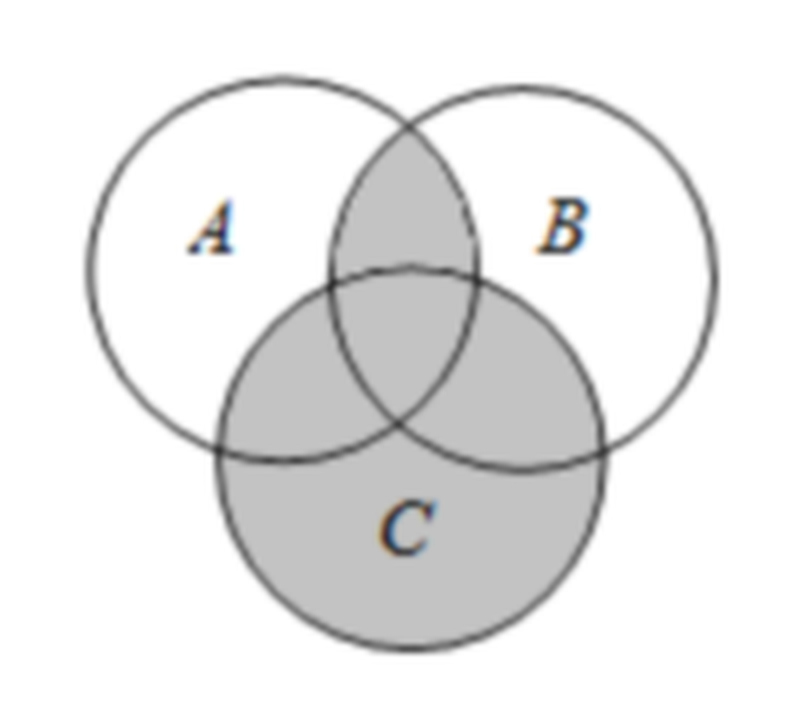
\includegraphics[width=0.30\textwidth]{figures/venn_ABcap_plus_C.png}
\end{center}

\keepwithprev
A. $(A\cup C)\cap(B\cup C)$\qquad B. $(A\cup B)\cap(A\cup C)$

C. $(A\cup B)\cap(B\cup C)$\qquad D. $(A\cup B)\cap C$

\ans{$A$}

\item 设 $f(x)=(x^2-6x+c_1)(x^2-6x+c_2)$，其中 $c_1\geqslant c_2$，集合

$M=\{x\mid f(x)=0\}=\{x_1,x_2,x_3\}\sub\Z$，则下列命题中不正确的是\mbox{（\quad）}

\keepwithprev
A. $3\in M$\qquad B. $c_2$ 可能为 $-16$

C. $c_1$ 可能为 $8$\qquad D. $M$ 中所有元素的和一定为 $9$

\ans{$C$}

\ifanswer
\solbegin
\step{若 $c_1$ 为 $8$，则 $c_2=9$，与 $c_1\geqslant c_2$ 矛盾，故选 $C$.}
\solend

\fi

\item 非空集合 $A$ 具有如下性质：①若 $x$、$y\in A$，则 $\dfrac{x}{y}\in A$；②若 $x$、$y\in A$，
则 $x+y\in A$；

由此可知：下列判断中，错误的是\mbox{（\quad）}

\keepwithprev
A. $-1\notin A$\qquad B. $\dfrac{2025}{2026}\in A$

C. 若 $x$、$y\in A$，则 $xy\in A$\qquad D. 若 $x$、$y\in A$，则 $x-y\in A$

\ans{$D$}

\ifanswer
\solbegin
\step{由题意得 $0\notin A$，$1\in A$，}
\step{对于 $A$，假设 $-1\in A$，则 $-1+1=0\in A$，矛盾，所以 $-1\notin A$，故 $A$ 正确；}
\step{对于 $B$，由 $1\in A$，得 $1+1=2\in A$，$2+1=3\in A$，$\cdots$，$2025\in A$，$2026\in A$，}
\step{所以 $\dfrac{2025}{2026}\in A$，故 $B$ 正确；}
\step{对于 $C$，因为 $1\in A$，$x\in A$，所以 $\dfrac1x\in A$，又因为 $y\in A$，
所以 $\dfrac{y}{\frac1x}=xy\in A$，}
\step{故 $C$ 正确；}
\step{对于 $D$，因为 $1\in A$，$2\in A$，若 $x=1$，$y=2$，则 $x-y=-1\notin A$，故 $D$ 错误.}
\step{故选 $D$.}
\solend

\fi

\end{enumerate}

\bigsec{三、解答题}

\begin{enumerate}
\setcounter{enumi}{13}

% 注：原卷本题题干把「$=0$」印在右花括号之外（$A=\{x\mid x^2-mx+4m-16\}=0$），
%     而其自己的【解析】印在括号之内（$A=\{x\mid x^2-mx+4m-16=0\}$）——原卷前后不一致，
%     本稿按解析与题目本意把 $=0$ 排在括号内，见文件头「排版差异」⑧。
\item 已知集合 $A=\{x\mid x^2-mx+4m-16=0\}$，$B=\{x\mid 1<x<4,x\in\N\}$，
$C=\{x\mid ax+2>0\}$，若 $A\cap B\neq\varnothing$，$A\cap C=\varnothing$，求实数 $m$ 的值以及
相应实数 $a$ 的取值范围.

\ifanswer
\solbegin
\step{集合 $A=\{x\mid x^2-mx+4m-16=0\}$，由 $\Delta=(-m)^2-4(4m-16)=(m-8)^2\geqslant0$，}
\step{所以当 $m=8$ 时，集合 $A=\{4\}$，当 $m\neq8$ 时，集合
$A=\left\{\dfrac{m-|m-8|}{2},\dfrac{m+|m-8|}{2}\right\}$，}
\step{集合 $B=\{x\mid 1<x<4,x\in\N\}$，得集合 $B=\{2,3\}$.}
\step{集合 $C=\{x\mid ax+2>0\}$，当 $a=0$ 时，集合 $C=\{x\mid x\in\R\}$，}
\step{当 $a<0$ 时，集合 $C=\left\{x\mid x<\dfrac2a\right\}$，当 $a>0$ 时，集合
$C=\left\{x\mid x>\dfrac2a\right\}$，}
\step{由 $A\cap B$ 非空得，$m=6$ 时，集合 $A=\{2,4\}$，$m=7$ 时，集合 $A=\{3,4\}$.}
\step{由 $A\cap C=\varnothing$，得 $m=6$ 或 $m=7$ 时，$a<0$ 或 $0<a<\dfrac12$ 符合要求.}
\solend

\fi

\ansspace[9]

\item 已知 $a>b>c$，$a+b+c=0$，方程 $ax^2+bx+c=0$ 的两个实根为 $x_1$、$x_2$.

\begin{enumerate}[label=(\arabic*)]
\item 证明：$-\dfrac12<\dfrac ba<1$；
% 注：此小问前加了 4pt 间距——不加时紧凑版该行的 $x_1^2$ 上标与下标恰好同箱，
%     pdftotext 抽正文会把上标当重影丢掉，make check 的正文指纹就对不上（纯抽取抖动，
%     版面与内容无差别，见 2026-09-20 入库注）。
\vspace{4pt}
\item 若 $x_1^2+x_1x_2+x_2^2=1$，求 $x_1^2-x_1x_2+x_2^2$.
\end{enumerate}

\ifanswer
\solbegin
\stepm{(1)}{因为 $a>b>c$，$a+b+c=0$，所以 $a>0$，$c<0$，$c=-a-b$，}
\step{由 $a>b$ 得 $\dfrac ba<1$ ①，由 $b>c$ 得 $b>-a-b$，即 $2b>-a$，即 $\dfrac ba>-\dfrac12$ ②，}
\step{由①②得 $-\dfrac12<\dfrac ba<1$；}
\stepm{(2)}{若 $x_1^2+x_1x_2+x_2^2=1$，则 $(x_1+x_2)^2-x_1x_2=1$，}
% 注：本行的连等式与原卷自己的结论对不上（照抄原卷、未改）——原卷印作
%     (b/a)²-b/a+1=1，则解出的应是 0 或 1；按 c=-a-b 应为 (b/a)²+b/a+1=1，
%     解得 0 或 -1（-1 因 c<0 舍去），恰与下一行「0 或 -1（舍去）」吻合。
%     详见文件头「原卷存疑」①。
\step{则 $\left(\dfrac ba\right)^2-\dfrac ca=\dfrac{b^2-ac}{a^2}
=\left(\dfrac ba\right)^2-\dfrac ba+1=1$，解得 $\dfrac ba=0$ 或 $-1$（舍去），}
\step{故 $\dfrac ba=0$，$\dfrac ca=-1$，}
\step{所以 $x_1^2-x_1x_2+x_2^2=(x_1+x_2)^2-3x_1x_2=\left(\dfrac ba\right)^2-3\times\dfrac ca=3$.}
\solend

\fi

\ansspace[6]

\item 已知方程 $x^2+px+q=0$ 与方程 $x^2+(p-3)x+2q+1=0$ 分别都有两个不相等的实根，若
他们的解集分别为 $A$、$B$，且 $A\cup B=\{1,2,5\}$，求 $p$、$q$、$A$、$B$.

\ifanswer
\solbegin
\step{两方程分别有两个不相等的实数根，而根的并集只有 $3$ 个元素，}
\step{则两方程有一公共根. 分类讨论：}
\stepm{（1）}{公共根为 $1$ 时，$x=1$ 分别代入两方程：}
\step{$\begin{cases}p+q+1=0\\ p-3+2q+1+1=0\end{cases}$，解得 $p=-3$，$q=2$，}
\step{两方程变为 $x^2-3x+2=0$，解得 $x=1$ 或 $x=2$，}
\step{$x^2-6x+5=0$ 解得 $x=1$ 或 $x=5$，满足题意.}
\stepm{（2）}{公共根为 $2$ 时，$x=2$ 分别代入两方程：}
\step{$\begin{cases}4+2p+q=0\\ 4+2p-6+2q+1=0\end{cases}$，解得 $p=-\dfrac92$，$q=5$，}
\step{第一个方程变为 $2x^2-9x+10=0$，解得 $x=2$ 或 $x=\dfrac52$，不满足题意，舍去.}
\stepm{（3）}{公共根为 $5$ 时，$x=5$ 分别代入两方程：}
\step{$\begin{cases}25+5p+q=0\\ 25+5p-15+2q+1=0\end{cases}$，解得 $p=-\dfrac{39}{5}$，$q=14$，}
\step{第一个方程变为 $5x^2-39x+70=0$，解得 $x=5$ 或 $x=\dfrac{14}{5}$，不满足题意，舍去.}
\step{综上，$p=-3$，$q=2$，$A=\{1,2\}$，$B=\{1,5\}$.}
\solend

\fi

\ansspace[8]

\item 对于集合 $A=\{a_1,a_2,\cdots,a_n\}(n\in\Z,n\geqslant3)$，其中每个元素均为正整数，如果
任意去掉其
中一个元素 $a_i(i=1,2,3\cdots,n)$ 之后，剩余的所有元素组成集合 $A_i(i=1,2,\cdots,n)$，并且
$A_i$ 都能分为两个集合 $B$ 和 $C$，满足 $B\cap C=\varnothing,B\cup C=A_i$，其中 $B$ 和 $C$
的所有元素之和相
等，就称集合 $A$ 为“可分集合”.

\begin{enumerate}[label=(\arabic*)]
\item 判断集合 $\{1,3,5,7,9,11,13\}$ 是否是“可分集合”（不必写过程）；
\item 用反证法证明：五个元素的集合 $A=\{a_1,a_2,a_3,a_4,a_5\}$ 一定不是“可分集合”；
\item 已知集合 $A=\{a_1,a_2,\cdots,a_n\}(n\in\Z,n\geqslant3)$ 是“可分集合”，求 $n$ 的最小值.
\end{enumerate}

\ifanswer
\solbegin
\stepm{(1)}{集合 $\{1,3,5,7,9,11,13\}$ 是“可分集合”；}
\stepm{(2)}{不妨设 $a_1<a_2<a_3<a_4<a_5$，}
\step{若去掉的元素为 $a_2$，将集合 $\{a_1,a_3,a_4,a_5\}$ 分成两个交集为空集的子集，}
\step{且两个子集元素之和相等，则有 $a_1+a_5=a_3+a_4$ ①，或者 $a_5=a_1+a_3+a_4$ ②；}
\step{若去掉的元素为 $a_1$，将集合 $\{a_2,a_3,a_4,a_5\}$ 分成两个交集为空集的子集，}
\step{且两个子集元素之和相等，则有 $a_2+a_5=a_3+a_4$ ③，或者 $a_5=a_2+a_3+a_4$ ④.}
\step{由①、③，得 $a_1=a_2$，矛盾；由①、④，得 $a_1=-a_2$，矛盾；}
\step{由②、③，得 $a_1=-a_2$，矛盾；由②、④，得 $a_1=a_2$ 矛盾.}
\step{因此当 $n=5$ 时，集合一定不是“可分集合”；}
\stepm{(3)}{①设集合 $A=\{a_1,a_2,\cdots,a_n\}$ 的所有元素之和为 $M$.}
\step{由题意得 $M-a_i(i=1,2,\cdots,n)$ 均为偶数，}
\step{因此 $a_i(i=1,2,\cdots,n)$ 均为奇数或偶数.}
\step{如果 $M$ 为奇数，则 $a_i(i=1,2,\cdots,n)$ 也均为奇数，}
\step{由于 $M=a_1+a_2+\cdots+a_n$，所以 $n$ 为奇数.}
\step{如果 $M$ 为偶数，则 $M-a_i(i=1,2,\cdots,n)$ 均为偶数，此时设 $a_i=2b_i$，}
\step{则 $\{b_1,b_2,\cdots,b_n\}$ 也是“可分集合”.}
\step{重复上述操作有限次，便可得各项均为奇数的“可分集合”，}
\step{此时各项之和也为奇数，则集合 $A$ 中元素个数 $n$ 为奇数.}
\step{综上所述，集合 $A$ 中元素个数为奇数.}
\step{②当 $n=3$ 时，显然任意集合 $\{a_1,a_2,a_3\}$ 不是“可分集合”.}
\step{当 $n=5$ 时，第（2）问已经证明不是“可分集合”.}
\step{当 $n=7$ 时，集合 $A=\{1,3,5,7,9,11,13\}$，}
\step{因为 $3+5+7+9=11+13$，$1+9+13=5+7+11$，$9+13=1+3+7+11$，}
\step{$1+3+5+11=7+13$，$1+9+11=3+5+13$，$3+7+9=1+5+13$，}
\step{$1+3+5+9=7+11$，则集合 $A$ 是“可分集合”，}
\step{所以集合 $A$ 中元素个数 $n$ 的最小值是 $7$.}
\solend

\fi

\ansspace*[10]

\end{enumerate}

\end{document}
"
%
% 原始材料是微信公众号图文（公众号「魔都数学加油站」连载「27学年高一 24」，2026-09-19 发布，
% 原文标题「27学年高一24——2026-2027年上海市复旦附中高一上周末作业3集合与逻辑、等式的性质」），
% 正文为 7 张 PNG 页（1080×1527，各页同尺寸）。原文本身就是一份**讲评版**——题目下方直接印出
% 【答案】或【解析】。试题文字、答案与解析均照原卷录入，未改内容。
% 卷面上的粉色斜水印「魔都数学加油站」属水印，未录入。
%
% 卷首标题：原卷印作「2026-2027 年复旦附中高一上周末作业 3」（公众号标题里有「上海市」三字，
% 卷面标题行没有，本稿照卷面），年份区间按全稿惯例排 en dash，前缀照原卷保留「年」。
%
% 与原卷的排版差异（均已在 README「说明」中交代）：
%   ① 原文自**第 3 题**起（第 1、2 题未在该文中发布），故本稿题号亦自 3 起；
%   ② 原卷本就印有「一、填空题」「二、选择题」「三、解答题」三节标题，本稿照原卷分节，
%      只把标题改排成全稿统一的「大节标题」样式；
%   ③ 原卷第 11 题的答案「A」直接印在题干末尾的括号内，第 12、13 题的括号空着、答案写在
%      解析末句「故选 C／D」里，本稿统一改为试卷版隐去、答案版以 \ans{} 给出（第 12、13 题
%      另附【解析】），使两版彻底分离；
%   ④ 原卷的集合／数集符号正体与粗体混用（第 8 题题干的 $\mathbf{R}$、第 9 题题干的
%      $\mathbf{N}$、第 12 题题干的 $\mathbf{Z}$ 为粗体，第 14 题解析的 $N$、$R$ 为斜体），
%      本稿按全稿惯例统一写作 $\R$、$\N$、$\Z$；
%   ⑤ 原卷填空的横线约两个字宽，本稿按全稿惯例统一排 \blankline[4.4em]；
%   ⑥ 第 11 题的 Venn 图原卷印在上一页末尾（第 10 题解析右侧、「二、选择题」标题旁），
%      本稿移至第 11 题题干之后；图取原卷截图、4× LANCZOS 放大
%      （figures/venn_ABcap_plus_C.png，阴影为 $A\cap B$ 的交与整个 $C$，即 $(A\cap B)\cup C$）；
%   ⑦ 原卷自印副标题「集合与逻辑、等式的性质」，本稿照录（与 高一14 同例，未改用惯例副标题）；
%   ⑧ 第 14 题题干原卷把「$=0$」印在右花括号**之外**（作
%      $A=\{x\mid x^2-mx+4m-16\}=0$），而它**自己的【解析】却印在括号之内**
%      （作 $A=\{x\mid x^2-mx+4m-16=0\}$）——原卷前后不一致；按原卷解析与题目本意，
%      本稿题干的 $=0$ 排在括号**之内**（与 高一b 第 13 题「原卷漏排 $A=$，本稿补上」同例）。
%
% 原卷存疑一处（已放大到能看清字形后核对，无法确证原意，本稿照抄原卷、未改）：
%   ① 第 15(2)【解析】的连等式印作
%      $\left(\frac ba\right)^2-\frac ca=\frac{b^2-ac}{a^2}=\left(\frac ba\right)^2-\frac ba+1=1$，
%      解得 $\frac ba=0$ 或 $-1$（舍去）——但由 $c=-a-b$ 应得 $\frac{b^2-ac}{a^2}
%      =\left(\frac ba\right)^2+\frac ba+1$（原卷把「$+\frac ba$」印成了「$-\frac ba$」）：
%      按原卷那行解出的是 $0$ 或 $1$，与其自己的结论「$0$ 或 $-1$」对不上；而按
%      $+\frac ba$ 解恰得 $0$ 或 $-1$（$-1$ 因 $c<0$ 舍去），与后文吻合。原卷显系笔误，
%      本稿照抄原卷（见源码中该处上方注释）。

\documentclass[a4paper,11pt]{article}
\usepackage{common}

\begin{document}

\examtitlest[3]{2026--2027 年复旦附中高一上周末作业 3}{集合与逻辑、等式的性质}

\bigsec{一、填空题}

\begin{enumerate}
\setcounter{enumi}{2}

\item 设 $M=\{x\mid y^2=x+2\}$，$N=\{x\mid y^2=-2x+8\}$，则 $M\cap N=$ \blankline[4.4em].

\ifanswer
\solbegin
\step{$M=[-2,+\infty)$，$N=(-\infty,4]$，则 $M\cap N=[-2,4]$.}
\solend

\fi

\item 若“$x\geqslant a$”是“$|x|\leqslant2$”的必要条件，则实数 $a$ 的取值集合是 \blankline[4.4em].

\ans{$(-\infty,-2]$}

\item 某校一年级的 $200$ 人中，爱好数学的有 $95$ 人，爱好体育的有 $156$ 人，则数学体育都爱好
的至少有 \blankline[4.4em] 人.

\ifanswer
\solbegin
\step{数学体育都爱好的至少有 $95+156-200=51$ 人.}
\solend

\fi

\item 已知 $x$ 为实数，且 $x^2+\dfrac{1}{x^2}=3$，则 $x^3+\dfrac{1}{x^3}$ 的值是 \blankline[4.4em].

\ifanswer
\solbegin
\step{因为 $x^2+\dfrac{1}{x^2}=\left(x+\dfrac1x\right)^2-2=3$，所以 $x+\dfrac1x=\pm\sqrt5$，}
\step{所以 $x^3+\dfrac{1}{x^3}=\left(x+\dfrac1x\right)\left(x^2-1+\dfrac{1}{x^2}\right)=\pm2\sqrt5$.}
\solend

\fi

\item 非空集合 $A=\{x\mid a+1\leqslant x<2a-1\}$，$B=\{x\mid-2\leqslant x\leqslant5\}$，
若 $A\sub(A\cap B)$，则 $a$ 的取值范围是 \blankline[4.4em].

\ifanswer
\solbegin
\step{当 $a+1<2a-1$，即 $a>2$ 时，$A\neq\varnothing$，由 $A\sub(A\cap B)$ 得 $A\sub B$，}
\step{得 $\begin{cases}a+1\geqslant-2\\ 2a-1\leqslant5\end{cases}$，解得 $-3\leqslant a\leqslant3$，所以 $2<a\leqslant3$.}
\solend

\fi

\item 已知集合 $\{x\mid(x-1)(x^2-x+a)=0,x\in\R\}$ 中的所有元素之和为 $1$，则实数 $a$ 的取值范
围是 \blankline[4.4em].

\ifanswer
\solbegin
\step{令 $x-1=0$，得 $x=1$，}
\stepm{①}{若 $x^2-x+a=0$ 无实数根，则 $\Delta=1-4a<0$，解得 $a>\dfrac14$，}
\step{此时集合只有元素 $1$，符合题意；}
\stepm{②}{若 $x^2-x+a=0$ 有两个相等的实数根，则 $\Delta=1-4a=0$，解得 $a=\dfrac14$，}
\step{此时方程为 $x^2-x+\dfrac14=0$，解得 $x=\dfrac12$，此时集合为 $\left\{1,\dfrac12\right\}$，不合题意；}
\stepm{③}{若 $x^2-x+a=0$ 有两个不相等的实数根，则 $\Delta=1-4a>0$，解得 $a<\dfrac14$，}
\step{设方程 $x^2-x+a=0$ 的两个实根分别为 $x_1,x_2$，则 $x_1+x_2=1$，}
\step{若 $x_1\neq1,x_2\neq1$，则集合为 $\{1,x_1,x_2\}$，不合题意，}
\step{若 $x_1=1$，则 $x_2=0$，此时集合为 $\{1,0\}$，符合题意，所以 $a=x_1x_2=0$，}
\step{综上所述，实数 $a$ 的取值范围是 $\{0\}\cup\left(\dfrac14,+\infty\right)$.}
\solend

\fi

\item 集合 $A=\{m\mid m=2k,k\in\N,1\leqslant k\leqslant50\}$，
$B=\{n\mid n=i+j,i<j,i\in A,j\in A\}$，则 $B$ 中元素的个数是 \blankline[4.4em].

\ifanswer
\solbegin
\step{$B$ 中最小元素是 $6$，最大元素是 $198$，则 $B$ 中元素的个数是 $\dfrac{198-6}{2}+1=97$.}
\solend

\fi

\item 关于 $(x,y,z)$ 的方程组
$\begin{cases}x^2+y^2+25z^2=6zx+8yz\\ 3x^2+2y^2+z^2=240\end{cases}$ 的解集为 \blankline[4.4em].

\ifanswer
\solbegin
\step{由上式得 $(x^2-6xz+9z^2)+(y^2-8yz+16z^2)=0$，}
\step{则 $(x-3z)^2+(y-4z)^2=0$，}
\step{所以 $(x,y,z)=(3t,4t,t)$，$t$ 为实数，代入下式中 $27\cdot t^2+32t^2+t^2=60t^2=240$，}
\step{则 $t^2=4$，$t=\pm2$，所以 $(x,y,z)=(6,8,2),(-6,-8,-2)$.}
\solend

\fi

\end{enumerate}

\bigsec{二、选择题}

\begin{enumerate}
\setcounter{enumi}{10}

\item 下列表示图形中的阴影部分的是\mbox{（\quad）}

\begin{center}
% 图取原卷截图、4× LANCZOS 放大（原卷把图印在上一页末尾，本稿移至此处，见文件头⑥）。
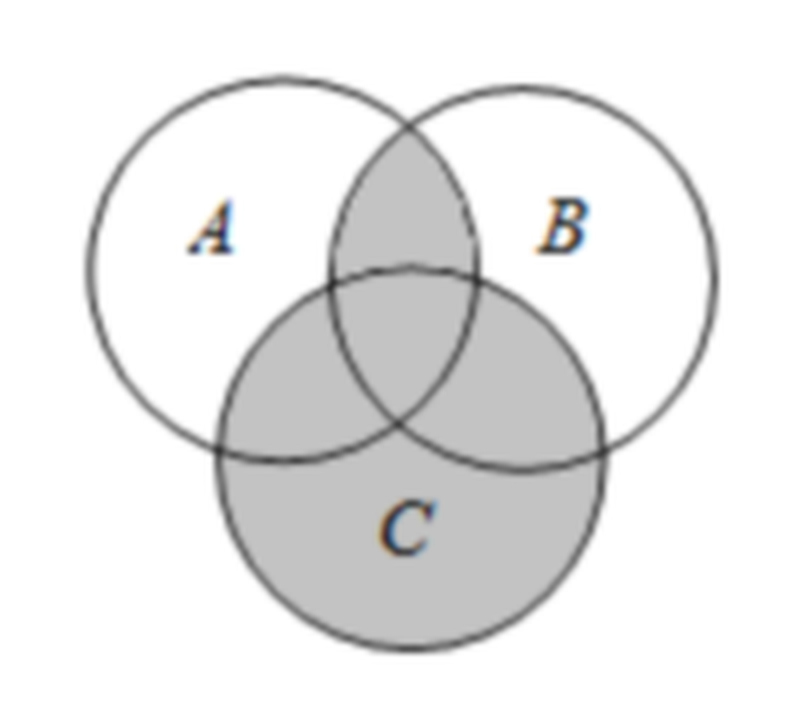
\includegraphics[width=0.30\textwidth]{figures/venn_ABcap_plus_C.png}
\end{center}

\keepwithprev
A. $(A\cup C)\cap(B\cup C)$\qquad B. $(A\cup B)\cap(A\cup C)$

C. $(A\cup B)\cap(B\cup C)$\qquad D. $(A\cup B)\cap C$

\ans{$A$}

\item 设 $f(x)=(x^2-6x+c_1)(x^2-6x+c_2)$，其中 $c_1\geqslant c_2$，集合

$M=\{x\mid f(x)=0\}=\{x_1,x_2,x_3\}\sub\Z$，则下列命题中不正确的是\mbox{（\quad）}

\keepwithprev
A. $3\in M$\qquad B. $c_2$ 可能为 $-16$

C. $c_1$ 可能为 $8$\qquad D. $M$ 中所有元素的和一定为 $9$

\ans{$C$}

\ifanswer
\solbegin
\step{若 $c_1$ 为 $8$，则 $c_2=9$，与 $c_1\geqslant c_2$ 矛盾，故选 $C$.}
\solend

\fi

\item 非空集合 $A$ 具有如下性质：①若 $x$、$y\in A$，则 $\dfrac{x}{y}\in A$；②若 $x$、$y\in A$，
则 $x+y\in A$；

由此可知：下列判断中，错误的是\mbox{（\quad）}

\keepwithprev
A. $-1\notin A$\qquad B. $\dfrac{2025}{2026}\in A$

C. 若 $x$、$y\in A$，则 $xy\in A$\qquad D. 若 $x$、$y\in A$，则 $x-y\in A$

\ans{$D$}

\ifanswer
\solbegin
\step{由题意得 $0\notin A$，$1\in A$，}
\step{对于 $A$，假设 $-1\in A$，则 $-1+1=0\in A$，矛盾，所以 $-1\notin A$，故 $A$ 正确；}
\step{对于 $B$，由 $1\in A$，得 $1+1=2\in A$，$2+1=3\in A$，$\cdots$，$2025\in A$，$2026\in A$，}
\step{所以 $\dfrac{2025}{2026}\in A$，故 $B$ 正确；}
\step{对于 $C$，因为 $1\in A$，$x\in A$，所以 $\dfrac1x\in A$，又因为 $y\in A$，
所以 $\dfrac{y}{\frac1x}=xy\in A$，}
\step{故 $C$ 正确；}
\step{对于 $D$，因为 $1\in A$，$2\in A$，若 $x=1$，$y=2$，则 $x-y=-1\notin A$，故 $D$ 错误.}
\step{故选 $D$.}
\solend

\fi

\end{enumerate}

\bigsec{三、解答题}

\begin{enumerate}
\setcounter{enumi}{13}

% 注：原卷本题题干把「$=0$」印在右花括号之外（$A=\{x\mid x^2-mx+4m-16\}=0$），
%     而其自己的【解析】印在括号之内（$A=\{x\mid x^2-mx+4m-16=0\}$）——原卷前后不一致，
%     本稿按解析与题目本意把 $=0$ 排在括号内，见文件头「排版差异」⑧。
\item 已知集合 $A=\{x\mid x^2-mx+4m-16=0\}$，$B=\{x\mid 1<x<4,x\in\N\}$，
$C=\{x\mid ax+2>0\}$，若 $A\cap B\neq\varnothing$，$A\cap C=\varnothing$，求实数 $m$ 的值以及
相应实数 $a$ 的取值范围.

\ifanswer
\solbegin
\step{集合 $A=\{x\mid x^2-mx+4m-16=0\}$，由 $\Delta=(-m)^2-4(4m-16)=(m-8)^2\geqslant0$，}
\step{所以当 $m=8$ 时，集合 $A=\{4\}$，当 $m\neq8$ 时，集合
$A=\left\{\dfrac{m-|m-8|}{2},\dfrac{m+|m-8|}{2}\right\}$，}
\step{集合 $B=\{x\mid 1<x<4,x\in\N\}$，得集合 $B=\{2,3\}$.}
\step{集合 $C=\{x\mid ax+2>0\}$，当 $a=0$ 时，集合 $C=\{x\mid x\in\R\}$，}
\step{当 $a<0$ 时，集合 $C=\left\{x\mid x<\dfrac2a\right\}$，当 $a>0$ 时，集合
$C=\left\{x\mid x>\dfrac2a\right\}$，}
\step{由 $A\cap B$ 非空得，$m=6$ 时，集合 $A=\{2,4\}$，$m=7$ 时，集合 $A=\{3,4\}$.}
\step{由 $A\cap C=\varnothing$，得 $m=6$ 或 $m=7$ 时，$a<0$ 或 $0<a<\dfrac12$ 符合要求.}
\solend

\fi

\ansspace[9]

\item 已知 $a>b>c$，$a+b+c=0$，方程 $ax^2+bx+c=0$ 的两个实根为 $x_1$、$x_2$.

\begin{enumerate}[label=(\arabic*)]
\item 证明：$-\dfrac12<\dfrac ba<1$；
% 注：此小问前加了 4pt 间距——不加时紧凑版该行的 $x_1^2$ 上标与下标恰好同箱，
%     pdftotext 抽正文会把上标当重影丢掉，make check 的正文指纹就对不上（纯抽取抖动，
%     版面与内容无差别，见 2026-09-20 入库注）。
\vspace{4pt}
\item 若 $x_1^2+x_1x_2+x_2^2=1$，求 $x_1^2-x_1x_2+x_2^2$.
\end{enumerate}

\ifanswer
\solbegin
\stepm{(1)}{因为 $a>b>c$，$a+b+c=0$，所以 $a>0$，$c<0$，$c=-a-b$，}
\step{由 $a>b$ 得 $\dfrac ba<1$ ①，由 $b>c$ 得 $b>-a-b$，即 $2b>-a$，即 $\dfrac ba>-\dfrac12$ ②，}
\step{由①②得 $-\dfrac12<\dfrac ba<1$；}
\stepm{(2)}{若 $x_1^2+x_1x_2+x_2^2=1$，则 $(x_1+x_2)^2-x_1x_2=1$，}
% 注：本行的连等式与原卷自己的结论对不上（照抄原卷、未改）——原卷印作
%     (b/a)²-b/a+1=1，则解出的应是 0 或 1；按 c=-a-b 应为 (b/a)²+b/a+1=1，
%     解得 0 或 -1（-1 因 c<0 舍去），恰与下一行「0 或 -1（舍去）」吻合。
%     详见文件头「原卷存疑」①。
\step{则 $\left(\dfrac ba\right)^2-\dfrac ca=\dfrac{b^2-ac}{a^2}
=\left(\dfrac ba\right)^2-\dfrac ba+1=1$，解得 $\dfrac ba=0$ 或 $-1$（舍去），}
\step{故 $\dfrac ba=0$，$\dfrac ca=-1$，}
\step{所以 $x_1^2-x_1x_2+x_2^2=(x_1+x_2)^2-3x_1x_2=\left(\dfrac ba\right)^2-3\times\dfrac ca=3$.}
\solend

\fi

\ansspace[6]

\item 已知方程 $x^2+px+q=0$ 与方程 $x^2+(p-3)x+2q+1=0$ 分别都有两个不相等的实根，若
他们的解集分别为 $A$、$B$，且 $A\cup B=\{1,2,5\}$，求 $p$、$q$、$A$、$B$.

\ifanswer
\solbegin
\step{两方程分别有两个不相等的实数根，而根的并集只有 $3$ 个元素，}
\step{则两方程有一公共根. 分类讨论：}
\stepm{（1）}{公共根为 $1$ 时，$x=1$ 分别代入两方程：}
\step{$\begin{cases}p+q+1=0\\ p-3+2q+1+1=0\end{cases}$，解得 $p=-3$，$q=2$，}
\step{两方程变为 $x^2-3x+2=0$，解得 $x=1$ 或 $x=2$，}
\step{$x^2-6x+5=0$ 解得 $x=1$ 或 $x=5$，满足题意.}
\stepm{（2）}{公共根为 $2$ 时，$x=2$ 分别代入两方程：}
\step{$\begin{cases}4+2p+q=0\\ 4+2p-6+2q+1=0\end{cases}$，解得 $p=-\dfrac92$，$q=5$，}
\step{第一个方程变为 $2x^2-9x+10=0$，解得 $x=2$ 或 $x=\dfrac52$，不满足题意，舍去.}
\stepm{（3）}{公共根为 $5$ 时，$x=5$ 分别代入两方程：}
\step{$\begin{cases}25+5p+q=0\\ 25+5p-15+2q+1=0\end{cases}$，解得 $p=-\dfrac{39}{5}$，$q=14$，}
\step{第一个方程变为 $5x^2-39x+70=0$，解得 $x=5$ 或 $x=\dfrac{14}{5}$，不满足题意，舍去.}
\step{综上，$p=-3$，$q=2$，$A=\{1,2\}$，$B=\{1,5\}$.}
\solend

\fi

\ansspace[8]

\item 对于集合 $A=\{a_1,a_2,\cdots,a_n\}(n\in\Z,n\geqslant3)$，其中每个元素均为正整数，如果
任意去掉其
中一个元素 $a_i(i=1,2,3\cdots,n)$ 之后，剩余的所有元素组成集合 $A_i(i=1,2,\cdots,n)$，并且
$A_i$ 都能分为两个集合 $B$ 和 $C$，满足 $B\cap C=\varnothing,B\cup C=A_i$，其中 $B$ 和 $C$
的所有元素之和相
等，就称集合 $A$ 为“可分集合”.

\begin{enumerate}[label=(\arabic*)]
\item 判断集合 $\{1,3,5,7,9,11,13\}$ 是否是“可分集合”（不必写过程）；
\item 用反证法证明：五个元素的集合 $A=\{a_1,a_2,a_3,a_4,a_5\}$ 一定不是“可分集合”；
\item 已知集合 $A=\{a_1,a_2,\cdots,a_n\}(n\in\Z,n\geqslant3)$ 是“可分集合”，求 $n$ 的最小值.
\end{enumerate}

\ifanswer
\solbegin
\stepm{(1)}{集合 $\{1,3,5,7,9,11,13\}$ 是“可分集合”；}
\stepm{(2)}{不妨设 $a_1<a_2<a_3<a_4<a_5$，}
\step{若去掉的元素为 $a_2$，将集合 $\{a_1,a_3,a_4,a_5\}$ 分成两个交集为空集的子集，}
\step{且两个子集元素之和相等，则有 $a_1+a_5=a_3+a_4$ ①，或者 $a_5=a_1+a_3+a_4$ ②；}
\step{若去掉的元素为 $a_1$，将集合 $\{a_2,a_3,a_4,a_5\}$ 分成两个交集为空集的子集，}
\step{且两个子集元素之和相等，则有 $a_2+a_5=a_3+a_4$ ③，或者 $a_5=a_2+a_3+a_4$ ④.}
\step{由①、③，得 $a_1=a_2$，矛盾；由①、④，得 $a_1=-a_2$，矛盾；}
\step{由②、③，得 $a_1=-a_2$，矛盾；由②、④，得 $a_1=a_2$ 矛盾.}
\step{因此当 $n=5$ 时，集合一定不是“可分集合”；}
\stepm{(3)}{①设集合 $A=\{a_1,a_2,\cdots,a_n\}$ 的所有元素之和为 $M$.}
\step{由题意得 $M-a_i(i=1,2,\cdots,n)$ 均为偶数，}
\step{因此 $a_i(i=1,2,\cdots,n)$ 均为奇数或偶数.}
\step{如果 $M$ 为奇数，则 $a_i(i=1,2,\cdots,n)$ 也均为奇数，}
\step{由于 $M=a_1+a_2+\cdots+a_n$，所以 $n$ 为奇数.}
\step{如果 $M$ 为偶数，则 $M-a_i(i=1,2,\cdots,n)$ 均为偶数，此时设 $a_i=2b_i$，}
\step{则 $\{b_1,b_2,\cdots,b_n\}$ 也是“可分集合”.}
\step{重复上述操作有限次，便可得各项均为奇数的“可分集合”，}
\step{此时各项之和也为奇数，则集合 $A$ 中元素个数 $n$ 为奇数.}
\step{综上所述，集合 $A$ 中元素个数为奇数.}
\step{②当 $n=3$ 时，显然任意集合 $\{a_1,a_2,a_3\}$ 不是“可分集合”.}
\step{当 $n=5$ 时，第（2）问已经证明不是“可分集合”.}
\step{当 $n=7$ 时，集合 $A=\{1,3,5,7,9,11,13\}$，}
\step{因为 $3+5+7+9=11+13$，$1+9+13=5+7+11$，$9+13=1+3+7+11$，}
\step{$1+3+5+11=7+13$，$1+9+11=3+5+13$，$3+7+9=1+5+13$，}
\step{$1+3+5+9=7+11$，则集合 $A$ 是“可分集合”，}
\step{所以集合 $A$ 中元素个数 $n$ 的最小值是 $7$.}
\solend

\fi

\ansspace*[10]

\end{enumerate}

\end{document}
"
%
% 原始材料是微信公众号图文（公众号「魔都数学加油站」连载「27学年高一 24」，2026-09-19 发布，
% 原文标题「27学年高一24——2026-2027年上海市复旦附中高一上周末作业3集合与逻辑、等式的性质」），
% 正文为 7 张 PNG 页（1080×1527，各页同尺寸）。原文本身就是一份**讲评版**——题目下方直接印出
% 【答案】或【解析】。试题文字、答案与解析均照原卷录入，未改内容。
% 卷面上的粉色斜水印「魔都数学加油站」属水印，未录入。
%
% 卷首标题：原卷印作「2026-2027 年复旦附中高一上周末作业 3」（公众号标题里有「上海市」三字，
% 卷面标题行没有，本稿照卷面），年份区间按全稿惯例排 en dash，前缀照原卷保留「年」。
%
% 与原卷的排版差异（均已在 README「说明」中交代）：
%   ① 原文自**第 3 题**起（第 1、2 题未在该文中发布），故本稿题号亦自 3 起；
%   ② 原卷本就印有「一、填空题」「二、选择题」「三、解答题」三节标题，本稿照原卷分节，
%      只把标题改排成全稿统一的「大节标题」样式；
%   ③ 原卷第 11 题的答案「A」直接印在题干末尾的括号内，第 12、13 题的括号空着、答案写在
%      解析末句「故选 C／D」里，本稿统一改为试卷版隐去、答案版以 \ans{} 给出（第 12、13 题
%      另附【解析】），使两版彻底分离；
%   ④ 原卷的集合／数集符号正体与粗体混用（第 8 题题干的 $\mathbf{R}$、第 9 题题干的
%      $\mathbf{N}$、第 12 题题干的 $\mathbf{Z}$ 为粗体，第 14 题解析的 $N$、$R$ 为斜体），
%      本稿按全稿惯例统一写作 $\R$、$\N$、$\Z$；
%   ⑤ 原卷填空的横线约两个字宽，本稿按全稿惯例统一排 \blankline[4.4em]；
%   ⑥ 第 11 题的 Venn 图原卷印在上一页末尾（第 10 题解析右侧、「二、选择题」标题旁），
%      本稿移至第 11 题题干之后；图取原卷截图、4× LANCZOS 放大
%      （figures/venn_ABcap_plus_C.png，阴影为 $A\cap B$ 的交与整个 $C$，即 $(A\cap B)\cup C$）；
%   ⑦ 原卷自印副标题「集合与逻辑、等式的性质」，本稿照录（与 高一14 同例，未改用惯例副标题）；
%   ⑧ 第 14 题题干原卷把「$=0$」印在右花括号**之外**（作
%      $A=\{x\mid x^2-mx+4m-16\}=0$），而它**自己的【解析】却印在括号之内**
%      （作 $A=\{x\mid x^2-mx+4m-16=0\}$）——原卷前后不一致；按原卷解析与题目本意，
%      本稿题干的 $=0$ 排在括号**之内**（与 高一b 第 13 题「原卷漏排 $A=$，本稿补上」同例）。
%
% 原卷存疑一处（已放大到能看清字形后核对，无法确证原意，本稿照抄原卷、未改）：
%   ① 第 15(2)【解析】的连等式印作
%      $\left(\frac ba\right)^2-\frac ca=\frac{b^2-ac}{a^2}=\left(\frac ba\right)^2-\frac ba+1=1$，
%      解得 $\frac ba=0$ 或 $-1$（舍去）——但由 $c=-a-b$ 应得 $\frac{b^2-ac}{a^2}
%      =\left(\frac ba\right)^2+\frac ba+1$（原卷把「$+\frac ba$」印成了「$-\frac ba$」）：
%      按原卷那行解出的是 $0$ 或 $1$，与其自己的结论「$0$ 或 $-1$」对不上；而按
%      $+\frac ba$ 解恰得 $0$ 或 $-1$（$-1$ 因 $c<0$ 舍去），与后文吻合。原卷显系笔误，
%      本稿照抄原卷（见源码中该处上方注释）。

\documentclass[a4paper,11pt]{article}
\usepackage{common}

\begin{document}

\examtitlest[3]{2026--2027 年复旦附中高一上周末作业 3}{集合与逻辑、等式的性质}

\bigsec{一、填空题}

\begin{enumerate}
\setcounter{enumi}{2}

\item 设 $M=\{x\mid y^2=x+2\}$，$N=\{x\mid y^2=-2x+8\}$，则 $M\cap N=$ \blankline[4.4em].

\ifanswer
\solbegin
\step{$M=[-2,+\infty)$，$N=(-\infty,4]$，则 $M\cap N=[-2,4]$.}
\solend

\fi

\item 若“$x\geqslant a$”是“$|x|\leqslant2$”的必要条件，则实数 $a$ 的取值集合是 \blankline[4.4em].

\ans{$(-\infty,-2]$}

\item 某校一年级的 $200$ 人中，爱好数学的有 $95$ 人，爱好体育的有 $156$ 人，则数学体育都爱好
的至少有 \blankline[4.4em] 人.

\ifanswer
\solbegin
\step{数学体育都爱好的至少有 $95+156-200=51$ 人.}
\solend

\fi

\item 已知 $x$ 为实数，且 $x^2+\dfrac{1}{x^2}=3$，则 $x^3+\dfrac{1}{x^3}$ 的值是 \blankline[4.4em].

\ifanswer
\solbegin
\step{因为 $x^2+\dfrac{1}{x^2}=\left(x+\dfrac1x\right)^2-2=3$，所以 $x+\dfrac1x=\pm\sqrt5$，}
\step{所以 $x^3+\dfrac{1}{x^3}=\left(x+\dfrac1x\right)\left(x^2-1+\dfrac{1}{x^2}\right)=\pm2\sqrt5$.}
\solend

\fi

\item 非空集合 $A=\{x\mid a+1\leqslant x<2a-1\}$，$B=\{x\mid-2\leqslant x\leqslant5\}$，
若 $A\sub(A\cap B)$，则 $a$ 的取值范围是 \blankline[4.4em].

\ifanswer
\solbegin
\step{当 $a+1<2a-1$，即 $a>2$ 时，$A\neq\varnothing$，由 $A\sub(A\cap B)$ 得 $A\sub B$，}
\step{得 $\begin{cases}a+1\geqslant-2\\ 2a-1\leqslant5\end{cases}$，解得 $-3\leqslant a\leqslant3$，所以 $2<a\leqslant3$.}
\solend

\fi

\item 已知集合 $\{x\mid(x-1)(x^2-x+a)=0,x\in\R\}$ 中的所有元素之和为 $1$，则实数 $a$ 的取值范
围是 \blankline[4.4em].

\ifanswer
\solbegin
\step{令 $x-1=0$，得 $x=1$，}
\stepm{①}{若 $x^2-x+a=0$ 无实数根，则 $\Delta=1-4a<0$，解得 $a>\dfrac14$，}
\step{此时集合只有元素 $1$，符合题意；}
\stepm{②}{若 $x^2-x+a=0$ 有两个相等的实数根，则 $\Delta=1-4a=0$，解得 $a=\dfrac14$，}
\step{此时方程为 $x^2-x+\dfrac14=0$，解得 $x=\dfrac12$，此时集合为 $\left\{1,\dfrac12\right\}$，不合题意；}
\stepm{③}{若 $x^2-x+a=0$ 有两个不相等的实数根，则 $\Delta=1-4a>0$，解得 $a<\dfrac14$，}
\step{设方程 $x^2-x+a=0$ 的两个实根分别为 $x_1,x_2$，则 $x_1+x_2=1$，}
\step{若 $x_1\neq1,x_2\neq1$，则集合为 $\{1,x_1,x_2\}$，不合题意，}
\step{若 $x_1=1$，则 $x_2=0$，此时集合为 $\{1,0\}$，符合题意，所以 $a=x_1x_2=0$，}
\step{综上所述，实数 $a$ 的取值范围是 $\{0\}\cup\left(\dfrac14,+\infty\right)$.}
\solend

\fi

\item 集合 $A=\{m\mid m=2k,k\in\N,1\leqslant k\leqslant50\}$，
$B=\{n\mid n=i+j,i<j,i\in A,j\in A\}$，则 $B$ 中元素的个数是 \blankline[4.4em].

\ifanswer
\solbegin
\step{$B$ 中最小元素是 $6$，最大元素是 $198$，则 $B$ 中元素的个数是 $\dfrac{198-6}{2}+1=97$.}
\solend

\fi

\item 关于 $(x,y,z)$ 的方程组
$\begin{cases}x^2+y^2+25z^2=6zx+8yz\\ 3x^2+2y^2+z^2=240\end{cases}$ 的解集为 \blankline[4.4em].

\ifanswer
\solbegin
\step{由上式得 $(x^2-6xz+9z^2)+(y^2-8yz+16z^2)=0$，}
\step{则 $(x-3z)^2+(y-4z)^2=0$，}
\step{所以 $(x,y,z)=(3t,4t,t)$，$t$ 为实数，代入下式中 $27\cdot t^2+32t^2+t^2=60t^2=240$，}
\step{则 $t^2=4$，$t=\pm2$，所以 $(x,y,z)=(6,8,2),(-6,-8,-2)$.}
\solend

\fi

\end{enumerate}

\bigsec{二、选择题}

\begin{enumerate}
\setcounter{enumi}{10}

\item 下列表示图形中的阴影部分的是\mbox{（\quad）}

\begin{center}
% 图取原卷截图、4× LANCZOS 放大（原卷把图印在上一页末尾，本稿移至此处，见文件头⑥）。
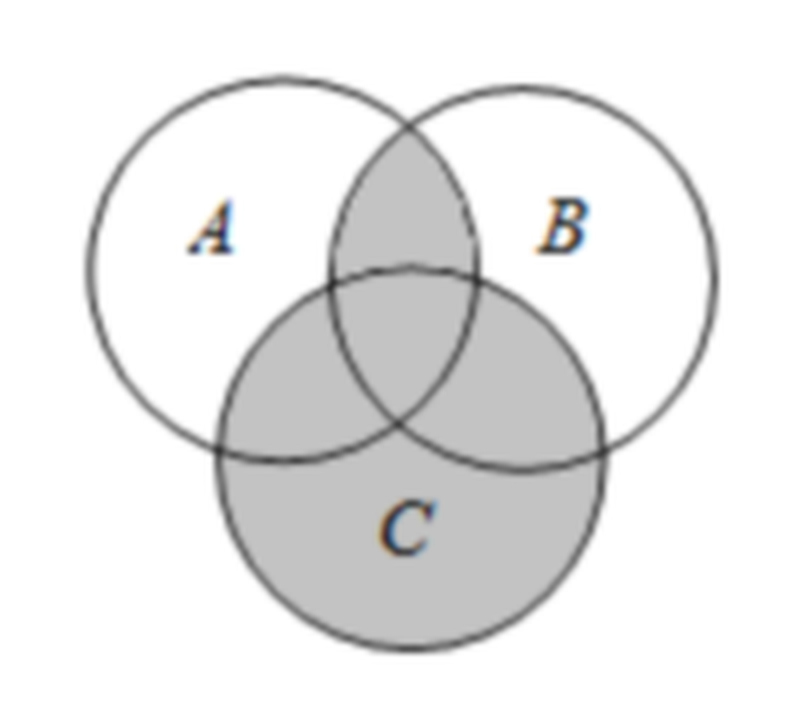
\includegraphics[width=0.30\textwidth]{figures/venn_ABcap_plus_C.png}
\end{center}

\keepwithprev
A. $(A\cup C)\cap(B\cup C)$\qquad B. $(A\cup B)\cap(A\cup C)$

C. $(A\cup B)\cap(B\cup C)$\qquad D. $(A\cup B)\cap C$

\ans{$A$}

\item 设 $f(x)=(x^2-6x+c_1)(x^2-6x+c_2)$，其中 $c_1\geqslant c_2$，集合

$M=\{x\mid f(x)=0\}=\{x_1,x_2,x_3\}\sub\Z$，则下列命题中不正确的是\mbox{（\quad）}

\keepwithprev
A. $3\in M$\qquad B. $c_2$ 可能为 $-16$

C. $c_1$ 可能为 $8$\qquad D. $M$ 中所有元素的和一定为 $9$

\ans{$C$}

\ifanswer
\solbegin
\step{若 $c_1$ 为 $8$，则 $c_2=9$，与 $c_1\geqslant c_2$ 矛盾，故选 $C$.}
\solend

\fi

\item 非空集合 $A$ 具有如下性质：①若 $x$、$y\in A$，则 $\dfrac{x}{y}\in A$；②若 $x$、$y\in A$，
则 $x+y\in A$；

由此可知：下列判断中，错误的是\mbox{（\quad）}

\keepwithprev
A. $-1\notin A$\qquad B. $\dfrac{2025}{2026}\in A$

C. 若 $x$、$y\in A$，则 $xy\in A$\qquad D. 若 $x$、$y\in A$，则 $x-y\in A$

\ans{$D$}

\ifanswer
\solbegin
\step{由题意得 $0\notin A$，$1\in A$，}
\step{对于 $A$，假设 $-1\in A$，则 $-1+1=0\in A$，矛盾，所以 $-1\notin A$，故 $A$ 正确；}
\step{对于 $B$，由 $1\in A$，得 $1+1=2\in A$，$2+1=3\in A$，$\cdots$，$2025\in A$，$2026\in A$，}
\step{所以 $\dfrac{2025}{2026}\in A$，故 $B$ 正确；}
\step{对于 $C$，因为 $1\in A$，$x\in A$，所以 $\dfrac1x\in A$，又因为 $y\in A$，
所以 $\dfrac{y}{\frac1x}=xy\in A$，}
\step{故 $C$ 正确；}
\step{对于 $D$，因为 $1\in A$，$2\in A$，若 $x=1$，$y=2$，则 $x-y=-1\notin A$，故 $D$ 错误.}
\step{故选 $D$.}
\solend

\fi

\end{enumerate}

\bigsec{三、解答题}

\begin{enumerate}
\setcounter{enumi}{13}

% 注：原卷本题题干把「$=0$」印在右花括号之外（$A=\{x\mid x^2-mx+4m-16\}=0$），
%     而其自己的【解析】印在括号之内（$A=\{x\mid x^2-mx+4m-16=0\}$）——原卷前后不一致，
%     本稿按解析与题目本意把 $=0$ 排在括号内，见文件头「排版差异」⑧。
\item 已知集合 $A=\{x\mid x^2-mx+4m-16=0\}$，$B=\{x\mid 1<x<4,x\in\N\}$，
$C=\{x\mid ax+2>0\}$，若 $A\cap B\neq\varnothing$，$A\cap C=\varnothing$，求实数 $m$ 的值以及
相应实数 $a$ 的取值范围.

\ifanswer
\solbegin
\step{集合 $A=\{x\mid x^2-mx+4m-16=0\}$，由 $\Delta=(-m)^2-4(4m-16)=(m-8)^2\geqslant0$，}
\step{所以当 $m=8$ 时，集合 $A=\{4\}$，当 $m\neq8$ 时，集合
$A=\left\{\dfrac{m-|m-8|}{2},\dfrac{m+|m-8|}{2}\right\}$，}
\step{集合 $B=\{x\mid 1<x<4,x\in\N\}$，得集合 $B=\{2,3\}$.}
\step{集合 $C=\{x\mid ax+2>0\}$，当 $a=0$ 时，集合 $C=\{x\mid x\in\R\}$，}
\step{当 $a<0$ 时，集合 $C=\left\{x\mid x<\dfrac2a\right\}$，当 $a>0$ 时，集合
$C=\left\{x\mid x>\dfrac2a\right\}$，}
\step{由 $A\cap B$ 非空得，$m=6$ 时，集合 $A=\{2,4\}$，$m=7$ 时，集合 $A=\{3,4\}$.}
\step{由 $A\cap C=\varnothing$，得 $m=6$ 或 $m=7$ 时，$a<0$ 或 $0<a<\dfrac12$ 符合要求.}
\solend

\fi

\ansspace[9]

\item 已知 $a>b>c$，$a+b+c=0$，方程 $ax^2+bx+c=0$ 的两个实根为 $x_1$、$x_2$.

\begin{enumerate}[label=(\arabic*)]
\item 证明：$-\dfrac12<\dfrac ba<1$；
% 注：此小问前加了 4pt 间距——不加时紧凑版该行的 $x_1^2$ 上标与下标恰好同箱，
%     pdftotext 抽正文会把上标当重影丢掉，make check 的正文指纹就对不上（纯抽取抖动，
%     版面与内容无差别，见 2026-09-20 入库注）。
\vspace{4pt}
\item 若 $x_1^2+x_1x_2+x_2^2=1$，求 $x_1^2-x_1x_2+x_2^2$.
\end{enumerate}

\ifanswer
\solbegin
\stepm{(1)}{因为 $a>b>c$，$a+b+c=0$，所以 $a>0$，$c<0$，$c=-a-b$，}
\step{由 $a>b$ 得 $\dfrac ba<1$ ①，由 $b>c$ 得 $b>-a-b$，即 $2b>-a$，即 $\dfrac ba>-\dfrac12$ ②，}
\step{由①②得 $-\dfrac12<\dfrac ba<1$；}
\stepm{(2)}{若 $x_1^2+x_1x_2+x_2^2=1$，则 $(x_1+x_2)^2-x_1x_2=1$，}
% 注：本行的连等式与原卷自己的结论对不上（照抄原卷、未改）——原卷印作
%     (b/a)²-b/a+1=1，则解出的应是 0 或 1；按 c=-a-b 应为 (b/a)²+b/a+1=1，
%     解得 0 或 -1（-1 因 c<0 舍去），恰与下一行「0 或 -1（舍去）」吻合。
%     详见文件头「原卷存疑」①。
\step{则 $\left(\dfrac ba\right)^2-\dfrac ca=\dfrac{b^2-ac}{a^2}
=\left(\dfrac ba\right)^2-\dfrac ba+1=1$，解得 $\dfrac ba=0$ 或 $-1$（舍去），}
\step{故 $\dfrac ba=0$，$\dfrac ca=-1$，}
\step{所以 $x_1^2-x_1x_2+x_2^2=(x_1+x_2)^2-3x_1x_2=\left(\dfrac ba\right)^2-3\times\dfrac ca=3$.}
\solend

\fi

\ansspace[6]

\item 已知方程 $x^2+px+q=0$ 与方程 $x^2+(p-3)x+2q+1=0$ 分别都有两个不相等的实根，若
他们的解集分别为 $A$、$B$，且 $A\cup B=\{1,2,5\}$，求 $p$、$q$、$A$、$B$.

\ifanswer
\solbegin
\step{两方程分别有两个不相等的实数根，而根的并集只有 $3$ 个元素，}
\step{则两方程有一公共根. 分类讨论：}
\stepm{（1）}{公共根为 $1$ 时，$x=1$ 分别代入两方程：}
\step{$\begin{cases}p+q+1=0\\ p-3+2q+1+1=0\end{cases}$，解得 $p=-3$，$q=2$，}
\step{两方程变为 $x^2-3x+2=0$，解得 $x=1$ 或 $x=2$，}
\step{$x^2-6x+5=0$ 解得 $x=1$ 或 $x=5$，满足题意.}
\stepm{（2）}{公共根为 $2$ 时，$x=2$ 分别代入两方程：}
\step{$\begin{cases}4+2p+q=0\\ 4+2p-6+2q+1=0\end{cases}$，解得 $p=-\dfrac92$，$q=5$，}
\step{第一个方程变为 $2x^2-9x+10=0$，解得 $x=2$ 或 $x=\dfrac52$，不满足题意，舍去.}
\stepm{（3）}{公共根为 $5$ 时，$x=5$ 分别代入两方程：}
\step{$\begin{cases}25+5p+q=0\\ 25+5p-15+2q+1=0\end{cases}$，解得 $p=-\dfrac{39}{5}$，$q=14$，}
\step{第一个方程变为 $5x^2-39x+70=0$，解得 $x=5$ 或 $x=\dfrac{14}{5}$，不满足题意，舍去.}
\step{综上，$p=-3$，$q=2$，$A=\{1,2\}$，$B=\{1,5\}$.}
\solend

\fi

\ansspace[8]

\item 对于集合 $A=\{a_1,a_2,\cdots,a_n\}(n\in\Z,n\geqslant3)$，其中每个元素均为正整数，如果
任意去掉其
中一个元素 $a_i(i=1,2,3\cdots,n)$ 之后，剩余的所有元素组成集合 $A_i(i=1,2,\cdots,n)$，并且
$A_i$ 都能分为两个集合 $B$ 和 $C$，满足 $B\cap C=\varnothing,B\cup C=A_i$，其中 $B$ 和 $C$
的所有元素之和相
等，就称集合 $A$ 为“可分集合”.

\begin{enumerate}[label=(\arabic*)]
\item 判断集合 $\{1,3,5,7,9,11,13\}$ 是否是“可分集合”（不必写过程）；
\item 用反证法证明：五个元素的集合 $A=\{a_1,a_2,a_3,a_4,a_5\}$ 一定不是“可分集合”；
\item 已知集合 $A=\{a_1,a_2,\cdots,a_n\}(n\in\Z,n\geqslant3)$ 是“可分集合”，求 $n$ 的最小值.
\end{enumerate}

\ifanswer
\solbegin
\stepm{(1)}{集合 $\{1,3,5,7,9,11,13\}$ 是“可分集合”；}
\stepm{(2)}{不妨设 $a_1<a_2<a_3<a_4<a_5$，}
\step{若去掉的元素为 $a_2$，将集合 $\{a_1,a_3,a_4,a_5\}$ 分成两个交集为空集的子集，}
\step{且两个子集元素之和相等，则有 $a_1+a_5=a_3+a_4$ ①，或者 $a_5=a_1+a_3+a_4$ ②；}
\step{若去掉的元素为 $a_1$，将集合 $\{a_2,a_3,a_4,a_5\}$ 分成两个交集为空集的子集，}
\step{且两个子集元素之和相等，则有 $a_2+a_5=a_3+a_4$ ③，或者 $a_5=a_2+a_3+a_4$ ④.}
\step{由①、③，得 $a_1=a_2$，矛盾；由①、④，得 $a_1=-a_2$，矛盾；}
\step{由②、③，得 $a_1=-a_2$，矛盾；由②、④，得 $a_1=a_2$ 矛盾.}
\step{因此当 $n=5$ 时，集合一定不是“可分集合”；}
\stepm{(3)}{①设集合 $A=\{a_1,a_2,\cdots,a_n\}$ 的所有元素之和为 $M$.}
\step{由题意得 $M-a_i(i=1,2,\cdots,n)$ 均为偶数，}
\step{因此 $a_i(i=1,2,\cdots,n)$ 均为奇数或偶数.}
\step{如果 $M$ 为奇数，则 $a_i(i=1,2,\cdots,n)$ 也均为奇数，}
\step{由于 $M=a_1+a_2+\cdots+a_n$，所以 $n$ 为奇数.}
\step{如果 $M$ 为偶数，则 $M-a_i(i=1,2,\cdots,n)$ 均为偶数，此时设 $a_i=2b_i$，}
\step{则 $\{b_1,b_2,\cdots,b_n\}$ 也是“可分集合”.}
\step{重复上述操作有限次，便可得各项均为奇数的“可分集合”，}
\step{此时各项之和也为奇数，则集合 $A$ 中元素个数 $n$ 为奇数.}
\step{综上所述，集合 $A$ 中元素个数为奇数.}
\step{②当 $n=3$ 时，显然任意集合 $\{a_1,a_2,a_3\}$ 不是“可分集合”.}
\step{当 $n=5$ 时，第（2）问已经证明不是“可分集合”.}
\step{当 $n=7$ 时，集合 $A=\{1,3,5,7,9,11,13\}$，}
\step{因为 $3+5+7+9=11+13$，$1+9+13=5+7+11$，$9+13=1+3+7+11$，}
\step{$1+3+5+11=7+13$，$1+9+11=3+5+13$，$3+7+9=1+5+13$，}
\step{$1+3+5+9=7+11$，则集合 $A$ 是“可分集合”，}
\step{所以集合 $A$ 中元素个数 $n$ 的最小值是 $7$.}
\solend

\fi

\ansspace*[10]

\end{enumerate}

\end{document}
"
%
% 原始材料是微信公众号图文（公众号「魔都数学加油站」连载「27学年高一 24」，2026-09-19 发布，
% 原文标题「27学年高一24——2026-2027年上海市复旦附中高一上周末作业3集合与逻辑、等式的性质」），
% 正文为 7 张 PNG 页（1080×1527，各页同尺寸）。原文本身就是一份**讲评版**——题目下方直接印出
% 【答案】或【解析】。试题文字、答案与解析均照原卷录入，未改内容。
% 卷面上的粉色斜水印「魔都数学加油站」属水印，未录入。
%
% 卷首标题：原卷印作「2026-2027 年复旦附中高一上周末作业 3」（公众号标题里有「上海市」三字，
% 卷面标题行没有，本稿照卷面），年份区间按全稿惯例排 en dash，前缀照原卷保留「年」。
%
% 与原卷的排版差异（均已在 README「说明」中交代）：
%   ① 原文自**第 3 题**起（第 1、2 题未在该文中发布），故本稿题号亦自 3 起；
%   ② 原卷本就印有「一、填空题」「二、选择题」「三、解答题」三节标题，本稿照原卷分节，
%      只把标题改排成全稿统一的「大节标题」样式；
%   ③ 原卷第 11 题的答案「A」直接印在题干末尾的括号内，第 12、13 题的括号空着、答案写在
%      解析末句「故选 C／D」里，本稿统一改为试卷版隐去、答案版以 \ans{} 给出（第 12、13 题
%      另附【解析】），使两版彻底分离；
%   ④ 原卷的集合／数集符号正体与粗体混用（第 8 题题干的 $\mathbf{R}$、第 9 题题干的
%      $\mathbf{N}$、第 12 题题干的 $\mathbf{Z}$ 为粗体，第 14 题解析的 $N$、$R$ 为斜体），
%      本稿按全稿惯例统一写作 $\R$、$\N$、$\Z$；
%   ⑤ 原卷填空的横线约两个字宽，本稿按全稿惯例统一排 \blankline[4.4em]；
%   ⑥ 第 11 题的 Venn 图原卷印在上一页末尾（第 10 题解析右侧、「二、选择题」标题旁），
%      本稿移至第 11 题题干之后；图取原卷截图、4× LANCZOS 放大
%      （figures/venn_ABcap_plus_C.png，阴影为 $A\cap B$ 的交与整个 $C$，即 $(A\cap B)\cup C$）；
%   ⑦ 原卷自印副标题「集合与逻辑、等式的性质」，本稿照录（与 高一14 同例，未改用惯例副标题）；
%   ⑧ 第 14 题题干原卷把「$=0$」印在右花括号**之外**（作
%      $A=\{x\mid x^2-mx+4m-16\}=0$），而它**自己的【解析】却印在括号之内**
%      （作 $A=\{x\mid x^2-mx+4m-16=0\}$）——原卷前后不一致；按原卷解析与题目本意，
%      本稿题干的 $=0$ 排在括号**之内**（与 高一b 第 13 题「原卷漏排 $A=$，本稿补上」同例）。
%
% 原卷存疑一处（已放大到能看清字形后核对，无法确证原意，本稿照抄原卷、未改）：
%   ① 第 15(2)【解析】的连等式印作
%      $\left(\frac ba\right)^2-\frac ca=\frac{b^2-ac}{a^2}=\left(\frac ba\right)^2-\frac ba+1=1$，
%      解得 $\frac ba=0$ 或 $-1$（舍去）——但由 $c=-a-b$ 应得 $\frac{b^2-ac}{a^2}
%      =\left(\frac ba\right)^2+\frac ba+1$（原卷把「$+\frac ba$」印成了「$-\frac ba$」）：
%      按原卷那行解出的是 $0$ 或 $1$，与其自己的结论「$0$ 或 $-1$」对不上；而按
%      $+\frac ba$ 解恰得 $0$ 或 $-1$（$-1$ 因 $c<0$ 舍去），与后文吻合。原卷显系笔误，
%      本稿照抄原卷（见源码中该处上方注释）。

\documentclass[a4paper,11pt]{article}
\usepackage{common}

\begin{document}

\examtitlest[3]{2026--2027 年复旦附中高一上周末作业 3}{集合与逻辑、等式的性质}

\bigsec{一、填空题}

\begin{enumerate}
\setcounter{enumi}{2}

\item 设 $M=\{x\mid y^2=x+2\}$，$N=\{x\mid y^2=-2x+8\}$，则 $M\cap N=$ \blankline[4.4em].

\ifanswer
\solbegin
\step{$M=[-2,+\infty)$，$N=(-\infty,4]$，则 $M\cap N=[-2,4]$.}
\solend

\fi

\item 若“$x\geqslant a$”是“$|x|\leqslant2$”的必要条件，则实数 $a$ 的取值集合是 \blankline[4.4em].

\ans{$(-\infty,-2]$}

\item 某校一年级的 $200$ 人中，爱好数学的有 $95$ 人，爱好体育的有 $156$ 人，则数学体育都爱好
的至少有 \blankline[4.4em] 人.

\ifanswer
\solbegin
\step{数学体育都爱好的至少有 $95+156-200=51$ 人.}
\solend

\fi

\item 已知 $x$ 为实数，且 $x^2+\dfrac{1}{x^2}=3$，则 $x^3+\dfrac{1}{x^3}$ 的值是 \blankline[4.4em].

\ifanswer
\solbegin
\step{因为 $x^2+\dfrac{1}{x^2}=\left(x+\dfrac1x\right)^2-2=3$，所以 $x+\dfrac1x=\pm\sqrt5$，}
\step{所以 $x^3+\dfrac{1}{x^3}=\left(x+\dfrac1x\right)\left(x^2-1+\dfrac{1}{x^2}\right)=\pm2\sqrt5$.}
\solend

\fi

\item 非空集合 $A=\{x\mid a+1\leqslant x<2a-1\}$，$B=\{x\mid-2\leqslant x\leqslant5\}$，
若 $A\sub(A\cap B)$，则 $a$ 的取值范围是 \blankline[4.4em].

\ifanswer
\solbegin
\step{当 $a+1<2a-1$，即 $a>2$ 时，$A\neq\varnothing$，由 $A\sub(A\cap B)$ 得 $A\sub B$，}
\step{得 $\begin{cases}a+1\geqslant-2\\ 2a-1\leqslant5\end{cases}$，解得 $-3\leqslant a\leqslant3$，所以 $2<a\leqslant3$.}
\solend

\fi

\item 已知集合 $\{x\mid(x-1)(x^2-x+a)=0,x\in\R\}$ 中的所有元素之和为 $1$，则实数 $a$ 的取值范
围是 \blankline[4.4em].

\ifanswer
\solbegin
\step{令 $x-1=0$，得 $x=1$，}
\stepm{①}{若 $x^2-x+a=0$ 无实数根，则 $\Delta=1-4a<0$，解得 $a>\dfrac14$，}
\step{此时集合只有元素 $1$，符合题意；}
\stepm{②}{若 $x^2-x+a=0$ 有两个相等的实数根，则 $\Delta=1-4a=0$，解得 $a=\dfrac14$，}
\step{此时方程为 $x^2-x+\dfrac14=0$，解得 $x=\dfrac12$，此时集合为 $\left\{1,\dfrac12\right\}$，不合题意；}
\stepm{③}{若 $x^2-x+a=0$ 有两个不相等的实数根，则 $\Delta=1-4a>0$，解得 $a<\dfrac14$，}
\step{设方程 $x^2-x+a=0$ 的两个实根分别为 $x_1,x_2$，则 $x_1+x_2=1$，}
\step{若 $x_1\neq1,x_2\neq1$，则集合为 $\{1,x_1,x_2\}$，不合题意，}
\step{若 $x_1=1$，则 $x_2=0$，此时集合为 $\{1,0\}$，符合题意，所以 $a=x_1x_2=0$，}
\step{综上所述，实数 $a$ 的取值范围是 $\{0\}\cup\left(\dfrac14,+\infty\right)$.}
\solend

\fi

\item 集合 $A=\{m\mid m=2k,k\in\N,1\leqslant k\leqslant50\}$，
$B=\{n\mid n=i+j,i<j,i\in A,j\in A\}$，则 $B$ 中元素的个数是 \blankline[4.4em].

\ifanswer
\solbegin
\step{$B$ 中最小元素是 $6$，最大元素是 $198$，则 $B$ 中元素的个数是 $\dfrac{198-6}{2}+1=97$.}
\solend

\fi

\item 关于 $(x,y,z)$ 的方程组
$\begin{cases}x^2+y^2+25z^2=6zx+8yz\\ 3x^2+2y^2+z^2=240\end{cases}$ 的解集为 \blankline[4.4em].

\ifanswer
\solbegin
\step{由上式得 $(x^2-6xz+9z^2)+(y^2-8yz+16z^2)=0$，}
\step{则 $(x-3z)^2+(y-4z)^2=0$，}
\step{所以 $(x,y,z)=(3t,4t,t)$，$t$ 为实数，代入下式中 $27\cdot t^2+32t^2+t^2=60t^2=240$，}
\step{则 $t^2=4$，$t=\pm2$，所以 $(x,y,z)=(6,8,2),(-6,-8,-2)$.}
\solend

\fi

\end{enumerate}

\bigsec{二、选择题}

\begin{enumerate}
\setcounter{enumi}{10}

\item 下列表示图形中的阴影部分的是\mbox{（\quad）}

\begin{center}
% 图取原卷截图、4× LANCZOS 放大（原卷把图印在上一页末尾，本稿移至此处，见文件头⑥）。
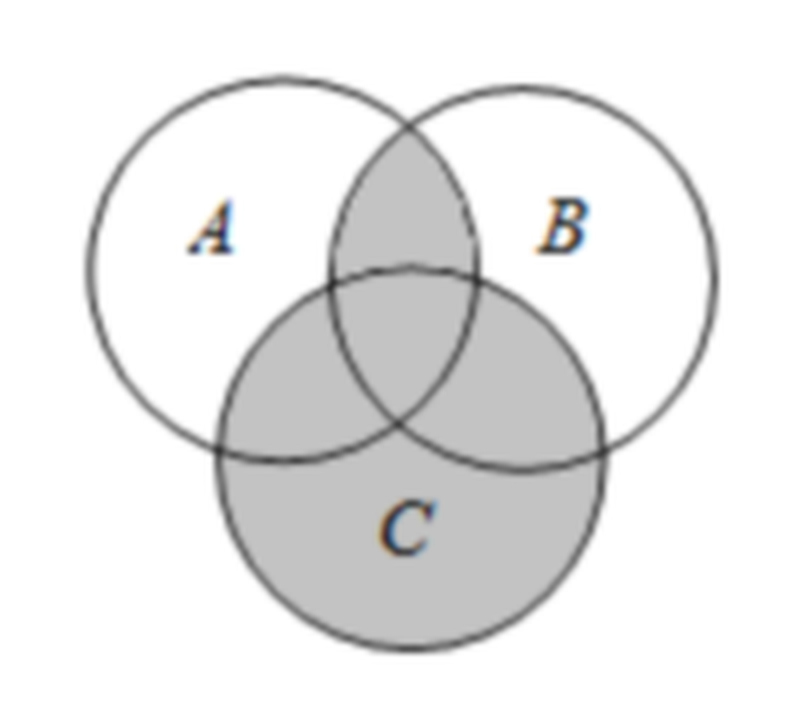
\includegraphics[width=0.30\textwidth]{figures/venn_ABcap_plus_C.png}
\end{center}

\keepwithprev
A. $(A\cup C)\cap(B\cup C)$\qquad B. $(A\cup B)\cap(A\cup C)$

C. $(A\cup B)\cap(B\cup C)$\qquad D. $(A\cup B)\cap C$

\ans{$A$}

\item 设 $f(x)=(x^2-6x+c_1)(x^2-6x+c_2)$，其中 $c_1\geqslant c_2$，集合

$M=\{x\mid f(x)=0\}=\{x_1,x_2,x_3\}\sub\Z$，则下列命题中不正确的是\mbox{（\quad）}

\keepwithprev
A. $3\in M$\qquad B. $c_2$ 可能为 $-16$

C. $c_1$ 可能为 $8$\qquad D. $M$ 中所有元素的和一定为 $9$

\ans{$C$}

\ifanswer
\solbegin
\step{若 $c_1$ 为 $8$，则 $c_2=9$，与 $c_1\geqslant c_2$ 矛盾，故选 $C$.}
\solend

\fi

\item 非空集合 $A$ 具有如下性质：①若 $x$、$y\in A$，则 $\dfrac{x}{y}\in A$；②若 $x$、$y\in A$，
则 $x+y\in A$；

由此可知：下列判断中，错误的是\mbox{（\quad）}

\keepwithprev
A. $-1\notin A$\qquad B. $\dfrac{2025}{2026}\in A$

C. 若 $x$、$y\in A$，则 $xy\in A$\qquad D. 若 $x$、$y\in A$，则 $x-y\in A$

\ans{$D$}

\ifanswer
\solbegin
\step{由题意得 $0\notin A$，$1\in A$，}
\step{对于 $A$，假设 $-1\in A$，则 $-1+1=0\in A$，矛盾，所以 $-1\notin A$，故 $A$ 正确；}
\step{对于 $B$，由 $1\in A$，得 $1+1=2\in A$，$2+1=3\in A$，$\cdots$，$2025\in A$，$2026\in A$，}
\step{所以 $\dfrac{2025}{2026}\in A$，故 $B$ 正确；}
\step{对于 $C$，因为 $1\in A$，$x\in A$，所以 $\dfrac1x\in A$，又因为 $y\in A$，
所以 $\dfrac{y}{\frac1x}=xy\in A$，}
\step{故 $C$ 正确；}
\step{对于 $D$，因为 $1\in A$，$2\in A$，若 $x=1$，$y=2$，则 $x-y=-1\notin A$，故 $D$ 错误.}
\step{故选 $D$.}
\solend

\fi

\end{enumerate}

\bigsec{三、解答题}

\begin{enumerate}
\setcounter{enumi}{13}

% 注：原卷本题题干把「$=0$」印在右花括号之外（$A=\{x\mid x^2-mx+4m-16\}=0$），
%     而其自己的【解析】印在括号之内（$A=\{x\mid x^2-mx+4m-16=0\}$）——原卷前后不一致，
%     本稿按解析与题目本意把 $=0$ 排在括号内，见文件头「排版差异」⑧。
\item 已知集合 $A=\{x\mid x^2-mx+4m-16=0\}$，$B=\{x\mid 1<x<4,x\in\N\}$，
$C=\{x\mid ax+2>0\}$，若 $A\cap B\neq\varnothing$，$A\cap C=\varnothing$，求实数 $m$ 的值以及
相应实数 $a$ 的取值范围.

\ifanswer
\solbegin
\step{集合 $A=\{x\mid x^2-mx+4m-16=0\}$，由 $\Delta=(-m)^2-4(4m-16)=(m-8)^2\geqslant0$，}
\step{所以当 $m=8$ 时，集合 $A=\{4\}$，当 $m\neq8$ 时，集合
$A=\left\{\dfrac{m-|m-8|}{2},\dfrac{m+|m-8|}{2}\right\}$，}
\step{集合 $B=\{x\mid 1<x<4,x\in\N\}$，得集合 $B=\{2,3\}$.}
\step{集合 $C=\{x\mid ax+2>0\}$，当 $a=0$ 时，集合 $C=\{x\mid x\in\R\}$，}
\step{当 $a<0$ 时，集合 $C=\left\{x\mid x<\dfrac2a\right\}$，当 $a>0$ 时，集合
$C=\left\{x\mid x>\dfrac2a\right\}$，}
\step{由 $A\cap B$ 非空得，$m=6$ 时，集合 $A=\{2,4\}$，$m=7$ 时，集合 $A=\{3,4\}$.}
\step{由 $A\cap C=\varnothing$，得 $m=6$ 或 $m=7$ 时，$a<0$ 或 $0<a<\dfrac12$ 符合要求.}
\solend

\fi

\ansspace[9]

\item 已知 $a>b>c$，$a+b+c=0$，方程 $ax^2+bx+c=0$ 的两个实根为 $x_1$、$x_2$.

\begin{enumerate}[label=(\arabic*)]
\item 证明：$-\dfrac12<\dfrac ba<1$；
% 注：此小问前加了 4pt 间距——不加时紧凑版该行的 $x_1^2$ 上标与下标恰好同箱，
%     pdftotext 抽正文会把上标当重影丢掉，make check 的正文指纹就对不上（纯抽取抖动，
%     版面与内容无差别，见 2026-09-20 入库注）。
\vspace{4pt}
\item 若 $x_1^2+x_1x_2+x_2^2=1$，求 $x_1^2-x_1x_2+x_2^2$.
\end{enumerate}

\ifanswer
\solbegin
\stepm{(1)}{因为 $a>b>c$，$a+b+c=0$，所以 $a>0$，$c<0$，$c=-a-b$，}
\step{由 $a>b$ 得 $\dfrac ba<1$ ①，由 $b>c$ 得 $b>-a-b$，即 $2b>-a$，即 $\dfrac ba>-\dfrac12$ ②，}
\step{由①②得 $-\dfrac12<\dfrac ba<1$；}
\stepm{(2)}{若 $x_1^2+x_1x_2+x_2^2=1$，则 $(x_1+x_2)^2-x_1x_2=1$，}
% 注：本行的连等式与原卷自己的结论对不上（照抄原卷、未改）——原卷印作
%     (b/a)²-b/a+1=1，则解出的应是 0 或 1；按 c=-a-b 应为 (b/a)²+b/a+1=1，
%     解得 0 或 -1（-1 因 c<0 舍去），恰与下一行「0 或 -1（舍去）」吻合。
%     详见文件头「原卷存疑」①。
\step{则 $\left(\dfrac ba\right)^2-\dfrac ca=\dfrac{b^2-ac}{a^2}
=\left(\dfrac ba\right)^2-\dfrac ba+1=1$，解得 $\dfrac ba=0$ 或 $-1$（舍去），}
\step{故 $\dfrac ba=0$，$\dfrac ca=-1$，}
\step{所以 $x_1^2-x_1x_2+x_2^2=(x_1+x_2)^2-3x_1x_2=\left(\dfrac ba\right)^2-3\times\dfrac ca=3$.}
\solend

\fi

\ansspace[6]

\item 已知方程 $x^2+px+q=0$ 与方程 $x^2+(p-3)x+2q+1=0$ 分别都有两个不相等的实根，若
他们的解集分别为 $A$、$B$，且 $A\cup B=\{1,2,5\}$，求 $p$、$q$、$A$、$B$.

\ifanswer
\solbegin
\step{两方程分别有两个不相等的实数根，而根的并集只有 $3$ 个元素，}
\step{则两方程有一公共根. 分类讨论：}
\stepm{（1）}{公共根为 $1$ 时，$x=1$ 分别代入两方程：}
\step{$\begin{cases}p+q+1=0\\ p-3+2q+1+1=0\end{cases}$，解得 $p=-3$，$q=2$，}
\step{两方程变为 $x^2-3x+2=0$，解得 $x=1$ 或 $x=2$，}
\step{$x^2-6x+5=0$ 解得 $x=1$ 或 $x=5$，满足题意.}
\stepm{（2）}{公共根为 $2$ 时，$x=2$ 分别代入两方程：}
\step{$\begin{cases}4+2p+q=0\\ 4+2p-6+2q+1=0\end{cases}$，解得 $p=-\dfrac92$，$q=5$，}
\step{第一个方程变为 $2x^2-9x+10=0$，解得 $x=2$ 或 $x=\dfrac52$，不满足题意，舍去.}
\stepm{（3）}{公共根为 $5$ 时，$x=5$ 分别代入两方程：}
\step{$\begin{cases}25+5p+q=0\\ 25+5p-15+2q+1=0\end{cases}$，解得 $p=-\dfrac{39}{5}$，$q=14$，}
\step{第一个方程变为 $5x^2-39x+70=0$，解得 $x=5$ 或 $x=\dfrac{14}{5}$，不满足题意，舍去.}
\step{综上，$p=-3$，$q=2$，$A=\{1,2\}$，$B=\{1,5\}$.}
\solend

\fi

\ansspace[8]

\item 对于集合 $A=\{a_1,a_2,\cdots,a_n\}(n\in\Z,n\geqslant3)$，其中每个元素均为正整数，如果
任意去掉其
中一个元素 $a_i(i=1,2,3\cdots,n)$ 之后，剩余的所有元素组成集合 $A_i(i=1,2,\cdots,n)$，并且
$A_i$ 都能分为两个集合 $B$ 和 $C$，满足 $B\cap C=\varnothing,B\cup C=A_i$，其中 $B$ 和 $C$
的所有元素之和相
等，就称集合 $A$ 为“可分集合”.

\begin{enumerate}[label=(\arabic*)]
\item 判断集合 $\{1,3,5,7,9,11,13\}$ 是否是“可分集合”（不必写过程）；
\item 用反证法证明：五个元素的集合 $A=\{a_1,a_2,a_3,a_4,a_5\}$ 一定不是“可分集合”；
\item 已知集合 $A=\{a_1,a_2,\cdots,a_n\}(n\in\Z,n\geqslant3)$ 是“可分集合”，求 $n$ 的最小值.
\end{enumerate}

\ifanswer
\solbegin
\stepm{(1)}{集合 $\{1,3,5,7,9,11,13\}$ 是“可分集合”；}
\stepm{(2)}{不妨设 $a_1<a_2<a_3<a_4<a_5$，}
\step{若去掉的元素为 $a_2$，将集合 $\{a_1,a_3,a_4,a_5\}$ 分成两个交集为空集的子集，}
\step{且两个子集元素之和相等，则有 $a_1+a_5=a_3+a_4$ ①，或者 $a_5=a_1+a_3+a_4$ ②；}
\step{若去掉的元素为 $a_1$，将集合 $\{a_2,a_3,a_4,a_5\}$ 分成两个交集为空集的子集，}
\step{且两个子集元素之和相等，则有 $a_2+a_5=a_3+a_4$ ③，或者 $a_5=a_2+a_3+a_4$ ④.}
\step{由①、③，得 $a_1=a_2$，矛盾；由①、④，得 $a_1=-a_2$，矛盾；}
\step{由②、③，得 $a_1=-a_2$，矛盾；由②、④，得 $a_1=a_2$ 矛盾.}
\step{因此当 $n=5$ 时，集合一定不是“可分集合”；}
\stepm{(3)}{①设集合 $A=\{a_1,a_2,\cdots,a_n\}$ 的所有元素之和为 $M$.}
\step{由题意得 $M-a_i(i=1,2,\cdots,n)$ 均为偶数，}
\step{因此 $a_i(i=1,2,\cdots,n)$ 均为奇数或偶数.}
\step{如果 $M$ 为奇数，则 $a_i(i=1,2,\cdots,n)$ 也均为奇数，}
\step{由于 $M=a_1+a_2+\cdots+a_n$，所以 $n$ 为奇数.}
\step{如果 $M$ 为偶数，则 $M-a_i(i=1,2,\cdots,n)$ 均为偶数，此时设 $a_i=2b_i$，}
\step{则 $\{b_1,b_2,\cdots,b_n\}$ 也是“可分集合”.}
\step{重复上述操作有限次，便可得各项均为奇数的“可分集合”，}
\step{此时各项之和也为奇数，则集合 $A$ 中元素个数 $n$ 为奇数.}
\step{综上所述，集合 $A$ 中元素个数为奇数.}
\step{②当 $n=3$ 时，显然任意集合 $\{a_1,a_2,a_3\}$ 不是“可分集合”.}
\step{当 $n=5$ 时，第（2）问已经证明不是“可分集合”.}
\step{当 $n=7$ 时，集合 $A=\{1,3,5,7,9,11,13\}$，}
\step{因为 $3+5+7+9=11+13$，$1+9+13=5+7+11$，$9+13=1+3+7+11$，}
\step{$1+3+5+11=7+13$，$1+9+11=3+5+13$，$3+7+9=1+5+13$，}
\step{$1+3+5+9=7+11$，则集合 $A$ 是“可分集合”，}
\step{所以集合 $A$ 中元素个数 $n$ 的最小值是 $7$.}
\solend

\fi

\ansspace*[10]

\end{enumerate}

\end{document}
